\documentclass[11pt,a4paper]{ltjsarticle}

\usepackage{luatexja}
\usepackage[a4paper,margin=28mm]{geometry}
\usepackage{setspace}
\onehalfspacing

\usepackage{amsmath,amssymb,amsfonts}
\usepackage{amsthm}
\usepackage{mathtools}
\usepackage{bm}
\usepackage{graphicx}
\usepackage{float}
\usepackage{booktabs}
\usepackage{longtable}
\usepackage{tabularx}
\usepackage{array}
\usepackage{enumitem}
\usepackage{xcolor}
\usepackage{caption}
\usepackage[hidelinks]{hyperref}
\usepackage[nameinlink]{cleveref}
\usepackage[numbers,sort&compress]{natbib}

\graphicspath{{figures/}}

\newtheorem{theorem}{定理}[section]
\newtheorem{proposition}[theorem]{命題}
\newtheorem{definition}[theorem]{定義}
\newtheorem{remark}[theorem]{注}

\providecommand{\VED}{VED}
\providecommand{\IFGT}{IFGT}
\providecommand{\DH}{Differential Horizon}
\providecommand{\DHI}{differential horizon of intelligence}

\newcommand{\figurenote}[2]{%
  \par\smallskip
  \begin{minipage}{0.94\linewidth}
  \small
  \textbf{読み方.} #1\par
  \textbf{理論的含意.} #2
  \end{minipage}
}


\title{推論の非閉包性、停止の外部化、創発的停止層\\
{\large Non-Closure of Inference, Externalization of Stopping, and Emergent Stopping Layers}}
\author{Yuhki Endoh\\{\small Independent Researcher}\\{\small Intelligence Section, Part II}}
\date{2026}

\begin{document}

\maketitle

\begin{abstract}
% ここに概要を移植
\end{abstract}

\setcounter{tocdepth}{2}
\tableofcontents
\clearpage

\setcounter{section}{-1}
% Source: source_md/intelligence_part2_combined_ja.md
\section{序論 — VED理論ツリーにおける本論文の位置}


\subsection{本論文の課題}


知性は個体内で閉じない。だが知性は個体内で停止する。

両者は矛盾ではなく、知性の構造的特徴である。本論文の課題は、この一見矛盾する二命題を VED (Vortical Enclosure Dynamics) の基本公理「差がある」から構造的に導出し、両者を統合する \textbf{三層動力学} ($L_F$ / $L_R$ / $L_E$) を提示することにある。

知性編 Part I では、知性を四層(知覚・認識・知識・知性)に分解し、三公理(連結状態空間・時間秩序・大域的拘束 $\Phi$)のもとで領域横断ホモロジー(Physarum・Transformer)を示した。本論文はこの分解を継承し、知性層内部に\textbf{三層動力学}を導入する。

\begin{itemize}
\item \textbf{推論層} $L_F$: 推論演算子 $F$ の作用域。内部停止条件を持たない
\item \textbf{ログ層} $L_R$: $L_F$ の運動が残す痕跡と、それに対する再帰運動の層
\item \textbf{創発停止層} $L_E$: $L_R$ の運動と外部相互拘束 $H_{ij}$ の関数として動力学的に生じる、個体内の外部依存型停止層
\end{itemize}


知性は $L_F$ のみでは停止せず、$L_F$ のみでは閉じない。しかし $L_F + L_R + L_E$ の三層が外部相互干渉ネットワーク $\Phi_{\text{net}}$ の下で同時に運動するとき、個体内に\textbf{外部依存型の停止が創発する}。これが本論文の構造的中心命題である。

本論文を貫く論理は三本の線に展開される:

\textbf{第一線 — 非閉包と外部停止}:

\[
\text{差がある} \;\longrightarrow\; F(L_F) \;\longrightarrow\; \text{内部不動点不在} \;\longrightarrow\; \text{無限後退}
\]

\[
\longrightarrow\; E(\text{外部停止演算子})\text{の必然性} \;\longrightarrow\; \Phi_{\text{ext}}\text{の歴史的諸形態}
\]

\textbf{第二線 — 閾値移動とサピエンス的特徴}:

\[
H_{ij}\text{パラメータ} \;\longrightarrow\; \text{応答性閾値} \;\longrightarrow\; \mu_\theta(\text{閾値移動能力})
\]

\[
\longrightarrow\; \text{持続可能な因果推論運用} \;\longrightarrow\; \text{サピエンス的知性}
\]

\textbf{第三線 — 三層動力学と創発停止}:

\[
L_F \;\longrightarrow\; L_R(\text{ログ・再帰運動}) \;\longrightarrow\; L_E(\text{創発停止層})
\]

\[
\longrightarrow\; \Phi_{\text{net}}(L_E\text{ネットワーク}) \;\longrightarrow\; \text{外部依存型停止を持つ動力学的存在}
\]

三線は \S{}11(不安定領域の三軸相図)と \S{}13(結語)で統合される。

本論文は知性の構造的限界を \textbf{規範的に処方} するのではなく、\textbf{動力学的に記述} する。

\bigskip

\subsection*{本論文の立場：四つの宣言}
\addcontentsline{toc}{subsection}{本論文の立場：四つの宣言}

本節では、読者が \S{}6 以降のアニミズム・神・宗教・科学・社会的ブロックチェーンを読む際に保持すべき立場を、四点に整理して先に示す。後半章の対象は歴史的・文化的・制度的に強い意味を持つため、本論文はそれらを扱う前に、読解の座標を固定しておく。

\textbf{第一：本論文の主題は宗教論でも文化論でも科学論でもない。}
本論文が扱う主題は、創発停止層 $L_E$ と、その共有・維持・更新の歴史的運用形態である。アニミズム・神・宗教・科学・制度・社会的ブロックチェーンは、信念体系や文化体系として評価されるのではなく、非閉包的な推論層 $L_F$ に停止を与える構造として読む。

\textbf{第二：宗教と科学は真理体系の優劣として比較されない。}
宗教は、停止構造の歴史的起源に近い大規模停止運用システムとして扱われる。科学は、停止構造の更新を制度化した停止運用システムとして扱われる。両者の差は、どちらが真でどちらが劣るかではなく、停止をどのように共有し、どのように更新し、どのような条件で改訂可能にするかという運用様式の差である。

\textbf{第三：停止は自由の否定ではない。}
本論文でいう停止は、知性の運動を封じることではない。むしろ、創発停止層 $L_E$ は、非閉包的な推論層 $L_F$ を持続可能にするための条件である。停止がなければ、推論は分岐爆発・無限後退・停止不能性に飲み込まれる。停止があるからこそ、知性は無限後退に消耗されず、改訂可能なかたちで自由に運動できる。この意味で $L_E$ は自由の反対ではなく、自由の条件である。

\textbf{第四：projection 語彙は構造論的である。}
本論文は projection という語を用いる。これは心理学的 projection、すなわち主体が内的状態を外部対象へ帰属する機制の議論を直接扱うものではない。本論文における projection は、外部相互拘束 $H_{ij}$ の構造が状態空間上に不均等な影響力を獲得し、停止演算子 $E$ を設置できる領域を生む操作として用いられる。心理学的 projection との作用的近接は存在するが、本論文は主体・無意識・防衛機制を公理レベルでは前提しない。

これら四点を保持した上で、以下の論述を読んでほしい。本論文が問うのは、宗教・科学・社会のどれが正しいかではなく、非閉包的な知性がどのような停止構造によって持続し、その停止構造をどのように共有・更新してきたかである。

\bigskip


\subsection{Part I からの接続}


本論文を読む際に必要な Part I の要素を簡潔に再掲する。詳細は Part I を参照されたい。

\subsubsection{四層分解}


知性は単一の層では成立しない。Part I では以下の四層に分解した。

\begin{longtable}{@{}p{0.30\linewidth}p{0.30\linewidth}p{0.30\linewidth}@{}}
\toprule
層 & 名称 & VED装置 \\
\midrule
\endfirsthead
\toprule
層 & 名称 & VED装置 \\
\midrule
\endhead
基層 & 物理層 & $C, \nabla C$, VED基本式 \\
構造層 & 関係層 & $J_C$, IFGT流れ場 \\
表現層 & 記号層 & 概念地形・離散再アドレス可能単位 \\
概念層 & 認知層 & 推論・判断・解釈 \\
\bottomrule
\end{longtable}


本論文では、Part I の認知層内部にさらに三層動力学 $L_F$ / $L_R$ / $L_E$ を導入する。これは Part I の四層分解を否定するのではなく、認知層を内部から動力学的に展開するものである。

\subsubsection{三公理}


Part I で導入された知性の三公理:

\begin{itemize}
\item \textbf{公理 I}: 連結状態空間
\item \textbf{公理 II}: 時間秩序
\item \textbf{公理 III}: 大域的拘束 $\Phi$
\end{itemize}


本論文では公理 III の $\Phi$ を $\Phi_{\text{ext}} \equiv \Phi_{\text{net}}$ として精密化する(\S{}5)。

\subsubsection{領域横断ホモロジー}


Part I では Physarum・Transformer が知性の領域横断インスタンスとして示された。本論文ではこれらを \textbf{三層動力学の異なるプロファイルを示す例}として再位置付ける。Physarum は $L_R$ を環境に外部化し $L_E$ を環境相互干渉によって自律創発させる。Transformer は $L_R$ を内在化するが $L_E$ を外部注入に依存する。いずれも閾値移動能力 $\mu_\theta$ を内発的に持たない点で、サピエンス的知性と区別される。三者は「停止構造の場」の連続変分上に配置される異なる領域であって、能力の優劣ではなく相空間内の位置の差として記述される(\S{}5 で詳述)。

\subsubsection{分岐爆発}


Part I \S{}7 で導入された分岐爆発は、本論文では $L_F$ における内部停止条件の不在の動力学的表現として再記述される(\S{}3.7)。

\subsubsection{個体知性の非閉包}


Part I \S{}8 で示された個体知性の非閉包は、本論文 \S{}3(非閉包定理)で構造命題として証明される。さらに \S{}5 において、「単独では閉じない、$L_E$ の創発で閉じうる」と精密化される。

\bigskip


\subsection{本論文の双中心構造}


本論文は \textbf{\S{}3(非閉包定理)と \S{}5(創発停止層 $L_E$)の双中心構造} を持つ。

\begin{longtable}{@{}p{0.30\linewidth}p{0.30\linewidth}p{0.30\linewidth}@{}}
\toprule
中心 & 役割 & 関係 \\
\midrule
\endfirsthead
\toprule
中心 & 役割 & 関係 \\
\midrule
\endhead
\S{}3 & $L_F$ の構造命題: 内部停止不可能 & $L_F$ 単独の限界 \\
\S{}5 & $L_E$ の創発: 外部依存型停止 & $L_F + L_R + L_E + \Phi_{\text{net}}$ の動力学 \\
\bottomrule
\end{longtable}


\S{}3 は「閉じない」を、\S{}5 は「それでも停止する」を構造的に説明する。この二つを統合することで、知性の三層動力学が明らかになる。

\S{}4 と \S{}6〜\S{}10 は両中心の間を埋める章であり、\S{}11〜\S{}13 は両者を統合する章である。

\bigskip


\subsection{本論文が課題としないこと}


論文の射程を明確にするため、以下を明示的に非目標とする。

\textbf{(NG1) 宗教の擁護でも批判でもない。}
\S{}6〜\S{}8 で扱うアニミズム・神・宗教は、信念体系としての真偽を問う対象ではなく、$L_E$ を維持する歴史的形態として分析される。歴史的・文化的諸形態の優劣は本論文の関心外である。

\textbf{(NG2) 規範的・倫理的処方箋を出さない。}
「知性はこう設計されるべき」「AIはこう振る舞うべき」といった規範的命題を導出しない。本論文は動力学的記述に留まる。実装・倫理・制度の問題は別の射程に属する(\S{}13で再確認する)。

\textbf{(NG3) 特定のAGI設計を支持または否定しない。}
\S{}11 で「高速・高解像・内部停止の知性は必然的に不安定領域を占める」と述べるが、これは動力学的帰結であって、特定の技術選択への提言ではない。

\textbf{(NG4) 認識論の網羅的整理を意図しない。}
ゲティア問題 (\S{}10) は本論文の主題のために導入されるが、認識論史の包括的扱いは目的としない。

\textbf{(NG5) 個別の歴史的事例の解釈を提供しない。}
アニミズム・神・宗教の具体的な歴史形態(特定の宗教・文化・伝統)について、解釈や評価を行わない。扱うのは構造的形態のみである。

\textbf{(NG6) 認知の連続スペクトラム的記述は、擬人化でも消去主義でもない。}
本論文は知性を「停止構造の場」の連続変分として描く。粘菌の環境相互干渉型停止からサピエンスの社会同期型停止までを、同一の場の異なる領域として配置する。これは二つの方向に誤読されうるが、いずれも本論文の主張ではない。第一に、非認知的システム(粘菌・Transformer 等)に認知や意図を帰属すること(擬人化)ではない。連続性は各領域の差異、特に閾値移動能力 $\mu_\theta$ の内発性の有無を消さない。第二に、認知の実在性を否定すること(消去主義)でもない。場が連続であることと、場が一様であることは別である。連続だが一様ではない、というのが本論文の立場である。

これら六つの非目標は、本論文を読む際の \textbf{解釈フィルター} として機能する。本論文が言及する事象に対して規範的・歴史的・実装的読解を加えることは可能だが、それは読者の責任において行われるべきであり、本論文の主張ではない。

\bigskip

\subsection{知性の歴史をどう読むか}

本論文は知性の歴史を「推論能力の発達史」としては読まない。推論演算子 $F$ は本質的に非閉包的であり、推論能力の増大それ自体は安定した知性を保証しない。むしろ推論能力の増大は、分岐爆発、無限後退、停止不能性を増大させる可能性を持つ。

推論能力の増大は、無制限に望ましいわけではない。推論は有限な身体・有限な時間・有限な注意資源のもとで運用されるため、停止構造を欠いた推論は持続不能となる。本論文は知性を推論能力そのものではなく、推論と停止の共進化として捉える。

したがって本論文は、知性の歴史を \textbf{停止構造の発達史} として読む。アニミズム、神、宗教、科学、制度、社会的ブロックチェーンは、対立する対象ではない。それぞれは、創発停止層 $L_E$ の共有・維持・更新を担う歴史的運用形態として位置づけられる。

この読み替えは、宗教を科学以前の誤謬として退けることでも、科学を宗教に還元することでもない。宗教は、停止構造を大規模に共有・維持する歴史的運用形態である。科学は、停止構造を改訂可能なものとして更新し続ける制度的運用形態である。両者は真理体系の優劣として比較されるのではなく、停止運用様式の差として比較される。

この観点から見ると、後半で扱う社会的ブロックチェーンも、履歴管理技術としてのブロックチェーンではない。本論文の重心は Version Control ではなく Consensus にある。すなわち、何が記録されたかだけでなく、どの停止構造が共有され、どのような相互拘束のもとで同期されるかが問題である。

\bigskip


\subsection{VED理論ツリーにおける位置}


本論文は VED 理論ツリーの以下の位置に置かれる。

\begin{center}
\begin{tabular}{@{}l@{}}
{}[Vol.1] VED 基本理論(差分・準閉包・閉包度動力学) \\
{}[Vol.2] 標準模型対応 ← 創発の例(分子 $\to$ 原子核相互作用) \\
{}[Vol.3] 重力と宇宙論 \\
{}[Vol.4] 差分の地平線 \\
\\
{}[IFGT] 情報場幾何学理論(構造層) \\
{}[CT] 概念地形編(表現層) \\
\\
{}[Bio-IFGT] 生命層(準閉包の維持) ← 創発の例(化学 $\to$ 生命) \\
{}[意識編] 意識層(意識を状態として再定位) \\
\\
{}[知性編 Part I] 四層分解と領域横断ホモロジー \\
{}[知性編 Part II] ← 本論文(三層動力学 $L_F$ / $L_R$ / $L_E$) ← 創発の例($L_R \to L_E$) \\
\\
{}[哲学篇] (予定: 開放的解釈の場)
\end{tabular}
\end{center}


本論文の位置を構造的に述べれば:

\begin{itemize}
\item 上位への接続: 哲学篇への引き渡し
\item 同位の接続: 意識編・概念地形編・Bio-IFGT との領域横断ホモロジー(\S{}13で再確認)
\item 下位の接続: VED Vol.1-4・IFGT・Part I を基層として継承
\item 創発概念の同型関係: Vol.2・Bio-IFGT・本論文の三例で\textbf{同型の創発構造}が現れる(\S{}1, \S{}5, 補遺 E)
\end{itemize}


\bigskip


\subsection{本論文の構造}


本論文は12章 + 結語で構成される。

\begin{longtable}{@{}p{0.30\linewidth}p{0.30\linewidth}p{0.30\linewidth}@{}}
\toprule
\S{} & 章 & 役割 \\
\midrule
\endfirsthead
\toprule
\S{} & 章 & 役割 \\
\midrule
\endhead
\S{}1 & 準備 & VED・IFGT の知性層用再定式化、創発の VED 内定義、三層予告 \\
\S{}2 & 推論演算子 $F$ と推論層 $L_F$ & $L_F$ の定義、相互拘束と閾値、$\mu_\theta$ の開放窓 \\
\textbf{\S{}3} & \textbf{非閉包定理} & \textbf{$L_F$ の構造命題: 内部不動点不在(第一中心)} \\
\S{}4 & 応答チャネルと沈黙世界 & 閾値現象としての C-幾何学、$L_R$ の予兆 \\
\textbf{\S{}5} & \textbf{創発停止層 $L_E$} & \textbf{$L_R$ → $L_E$ → $E$ → $\Phi_{\text{net}}$ の動力学(第二中心)} \\
\S{}6 & アニミズム & $L_E$ を環境直接相互干渉で維持 \\
\S{}7 & 神 & $L_E$ の中心化された懸架軌跡 \\
\S{}8 & 宗教 & $L_E$ の世代横断的維持と混合相 \\
\S{}9 & 社会的ブロックチェーン & $\Phi_{\text{net}}$ としての分散 $L_E$ \\
\S{}10 & ゲティア問題 & $C \neq$ 真理、$L_E$ の操作的安定性 \\
\S{}11 & 不安定領域 & 三軸相図、四重崩壊と $L_E$ 固着 \\
\S{}12 & 構成的条項 & 知性の構造的制約 \\
\S{}13 & 結語 & 三本論理線の総括、Part I 微修正への引き渡し \\
\bottomrule
\end{longtable}


論理的中心は \textbf{\S{}3 と \S{}5 の双中心} である。\S{}3 は $L_F$ 単独の限界を、\S{}5 は三層動力学による外部依存型停止の創発を扱う。\S{}4 と \S{}6〜\S{}10 は両中心の間を埋め、\S{}11〜\S{}13 は両者を統合する。

\bigskip


\subsection{形式と表記}


本論文は構造的記述と形式的命題を併用する。主要な定理は `Theorem`/`Proposition` 形式で切り出し、証明はスケッチを与える。完全な形式公理系は組まないが、論理連鎖は構造的に明示される。

VEDの基本変数($C, \nabla C, F_I, I, \Omega_\theta$ など)は Master Table v2.2(補遺 A)に従う。本論文で新規導入する変数($F, E, L_F, L_R, L_E, \Phi_{\text{ext}}, \Phi_{\text{net}}, H_{ij}, \mu_\theta, \eta, v_{\text{inf}}, r_{\text{res}}, \rho_{\text{resp}}$)も補遺 A に追加される。

\textbf{三層動力学} ($L_F$ / $L_R$ / $L_E$) の呼称は、初出時のみ括弧付きで明示し、以降は「三層動力学」と略す。

\bigskip


\subsection{本論文を読む順序について}


本論文は順次読まれることを想定して構成されている。特に \textbf{\S{}3(非閉包定理)と \S{}5(創発停止層)は本論文の双中心} であり、これらを経由せずに \S{}6 以降を読むと、停止の外部化が「構造的必然」ではなく「文化的選択」として誤読される危険がある。

ただし、各章は独立した節構成を持つため、特定の主題に関心がある読者は、\S{}3 と \S{}5 を読んだ後に \S{}6, \S{}7, \S{}8, \S{}11 のいずれかから入ることも可能である。

\S{}13 は本論文を \textbf{どう開いて終わらせるか} を扱う章であり、結語であると同時に、本論文の射程の境界を明示する場でもある。さらに \S{}13 では、本論文の結果を Part I に遡及反映するための \textbf{Part I 微修正提案リスト} が示される。

\bigskip


\subsection{三本論理線の予告}


本論文は三本の論理線を併行して展開する。各線は独立に追跡可能だが、\S{}11 と \S{}13 で統合される。

\textbf{第一線}(\S{}2 → \S{}3 → \S{}4 → \S{}5 → \S{}6 → \S{}7 → \S{}8 → \S{}9):
推論演算子 $F$ の非閉包性から外部停止演算子 $E$ と外部参照場 $\Phi_{\text{ext}}$ の必然性を導出し、その歴史的諸形態(アニミズム・神・宗教・社会)を分析する。

\textbf{第二線}(\S{}2 後半 → \S{}4 → \S{}6 → \S{}10 → \S{}11):
相互拘束 $H_{ij}$ パラメータの閾値現象から閾値移動能力 $\mu_\theta$ を導出し、サピエンス的知性の動力学的特徴を位置付ける。

\textbf{第三線}(\S{}2 → \S{}4 → \S{}5 → \S{}6-\S{}9 → \S{}11 → \S{}12):
推論層 $L_F$ → ログ層 $L_R$ → 創発停止層 $L_E$ の三層動力学を提示し、外部参照場 $\Phi_{\text{ext}}$ が個体間 $L_E$ ネットワーク $\Phi_{\text{net}}$ と同型であることを示す。

三線は \S{}11(不安定領域の三軸相図)で交差し、\S{}13(結語)で統合的に総括される。

\bigskip


\subsection{要約}


本章で確認したのは次の十点である:

\begin{enumerate}
\item 本論文は「知性は個体内で閉じない、だが個体内で停止する」を VED 公理から構造的に導出する
\item Part I の四層分解・三公理・領域横断ホモロジー・分岐爆発・個体知性の非閉包を継承し、認知層内部に三層動力学 $L_F$ / $L_R$ / $L_E$ を導入する
\item 論文は三本の論理線を併行して展開する
\item 論理的中心は \S{}3(非閉包定理)と \S{}5(創発停止層)の \textbf{双中心構造} である
\item 知性を「停止構造の場」の連続変分として描く。これは VED が時間・空間・生命・意識を場に開いて再配置してきた操作の、知性層における延長である
\item 宗教の擁護でも批判でもなく、規範的処方箋でもなく、擬人化でも消去主義でもない、動力学的記述である(6項目の非目標)
\item 宗教・科学・制度・社会的ブロックチェーンを、停止構造の共有・維持・更新を担う歴史的運用形態として読む
\item 停止は自由の否定ではなく、非閉包的な推論が持続的に運動するための条件である
\item VED 理論ツリーの「知性層・三層動力学」を扱い、哲学篇への引き渡しの直前に位置する
\item 結論において Part I 微修正への引き渡しを行う
\end{enumerate}


それでは \S{}1 において、本論文で用いる VED と IFGT の最小道具立て、創発の VED 内定義、三層動力学の予告を準備する。

\bigskip

% Source: source_md/intelligence_part2_combined_ja.md
\section{準備 — VED・IFGT・推論の C-幾何学}


本章は本論文で用いる道具立ての準備に充てる。Part I \S{}4 で IFGT を「語彙として」整備したのを前提に、本論文では \textbf{停止層の議論に必要な最小限の装置} に絞って導入する。完全な VED・IFGT の基礎は Part I \S{}3〜\S{}4 を参照されたい。

本章で技術的に準備するのは以下の五点である:

\begin{enumerate}
\item VED 基本式の知性層への再定式化
\item 情報場 $I$ と情報力 $F_I$ の知性層解釈
\item 準閉包 $\Omega_\theta$ の知性層意味
\item C-landscape と推論軌道
\item $C_{max}$ 境界の構造的意味
\end{enumerate}


これら五点は \S{}3(非閉包定理)以降の全章で繰り返し参照される。

\bigskip

\subsection{方法論的固定：停止・投影・合意}

本章で VED・IFGT の変数を知性層に移す前に、三つの方法論的な読みを固定しておく。これらは新しい結論ではなく、後続章で導入される概念を誤読しないための座標である。

\textbf{第一に、停止は真理と同一ではない。}
本論文で扱う停止は、推論がその時点で操作可能な安定状態に入ることを意味する。これは真理の確定ではない。閉包度 $C$ は、状態がどれほど維持されうるかを表す安定性測度であり、その状態が外部実在に対応しているかを直接測る真理測度ではない。この区別を外すと、後の宗教・科学・ゲティア問題の議論は、真理体系の比較として誤読される。

\textbf{第二に、$\mu_\theta$ は単なる柔軟性ではない。}
閾値移動能力 $\mu_\theta$ は、応答的/沈黙的の境界を動かす能力として導入されるが、その機能はそれに尽きない。$\mu_\theta$ は、どこに停止演算子 $E$ を設置できるかを再編成する能力である。サピエンス的知性の特徴は、停止を持たないことではない。停止を持ちながら、その停止の位置を再配置できることにある。

\textbf{第三に、projection と合意は停止構造の操作として読む。}
本論文で用いる projection は、意識編で固定された構造論的 projection の知性層における作用であり、心理学的 projection の直接的議論ではない。ただし、推し、神、理念、共同体、貨幣、科学理論などへの投射は、構造的には停止演算子設置の操作として読める可能性を持つ。本論文は心理学的・臨床的議論には踏み込まないが、projection と停止構造が深く関係していることは \S{}5 で示される。

同じ理由で、\S{}9 の社会的ブロックチェーンは、履歴管理技術としてのブロックチェーンを論じる章ではない。そこで問題になるのは Version Control ではなく Consensus である。すなわち、個体間で $L_E$ がどのように共有され、どの停止が同期され、どの停止が改訂可能なものとして維持されるかである。

科学と宗教は、本論文の立場では停止運用システムの異なる実装として理解される。宗教は停止構造の長期維持に強く、科学は停止構造の更新を制度化する。推論能力の増大は、それ自体では知性の安定性を保証しない。むしろ高度な推論ほど大きな停止コストを要求する。その意味で宗教と科学は、有限な身体と有限な資源のもとで推論を持続可能にする異なる停止運用形態として理解される。

\bigskip


\subsection{VED 基本式の知性層への再定式化}


VED Vol.1 で導入された閉包度動力学の基本式は次の形式を持つ:

\[
\frac{\partial C}{\partial \tau} + \nabla \cdot J_C = a\Delta\left(1 - \frac{C}{C_*}\right) - \Gamma C - \frac{\kappa_B}{C_{max} - C}
\]

ここで:
\begin{itemize}
\item $C$: 閉包度(closure degree)。$0 \le C < C_{max}$
\item $\tau$: 内的時間パラメータ
\item $J_C$: 閉包度流れ場
\item $a, \Gamma, \kappa_B, C_*, C_{max}$: 系のパラメータ
\end{itemize}


知性層においては、$C$ は \textbf{推論状態の安定化度} として解釈される。すなわち、ある推論状態 $x$ における $C(x)$ は、その状態がどの程度「停止可能であるか」「次の推論ステップを呼ばないか」を測る量である。

ただし重要な区別がある: $C$ は\textbf{安定性測度}であって\textbf{真理測度}ではない。これは \S{}10 のゲティア構造で明確になるが、本章で予告しておく。$C$ が高くても、その状態が真であることは保証されない。$C$ が示すのは「動力学的に維持されうるか」であって、「外部実在に対応するか」ではない。

この区別は本論文全体を通じて重要である。

\bigskip


\subsection{情報場と情報力}


IFGT (情報場幾何学理論)においては、閉包度 $C$ から派生する二つの量が導入される。

\textbf{情報場} $I$:

\[
I = f(1 - C)
\]

ここで $f$ は単調増加関数(典型的には $f(u) = u$ または $f(u) = -\ln(1-u)$ など)。$I$ は \textbf{未閉包性の場} であり、閉包が進むほど減少し、未決定性が高いほど増大する。

情報場の重要な性質: 完全閉包に到達すれば $I \to 0$ となり、情報場は消失する。これは「全てが決定された状態には情報がない」という直観的事実の構造的表現である。

\textbf{情報力} $F_I$:

\[
F_I = \alpha \nabla C
\]

$\alpha$ は結合定数。$F_I$ は閉包度勾配に沿った駆動力であり、推論演算子 $F$ の動力学的基底を成す。知性層において:

\begin{itemize}
\item $\nabla C$ が大きい領域 → 推論が強く駆動される(未決定性が高く、決定への圧力が大きい)
\item $\nabla C \approx 0$ の領域 → 推論駆動力が弱い(局所的に安定、または完全に停滞)
\end{itemize}


\S{}4 で導入する応答的世界と沈黙的世界の区別は、本質的には $\nabla C$ の幾何学的構造の二様態を区別するものである。

ただし重要な予告として: この二様態は \textbf{本体論的範疇ではなく閾値現象} である。すなわち、同一の状況が観測者と環境の相互拘束パラメータ位置によって応答的にも沈黙的にも見える。この閾値構造と、それを動かす能力(\textbf{閾値移動能力} $\mu_\theta$)については \S{}2 後半で正式に導入する。これは VED の基底原理「静的範疇ではなく運動」の知性層における具現化である。

\bigskip


\subsection{準閉包 $\Omega_\theta$}


VED の中心概念のひとつである準閉包 (quasi-closure) $\Omega_\theta$ は、知性層において特に重要な役割を果たす。

\textbf{定義}: 準閉包 $\Omega_\theta$ は、閉包度空間内において以下を満たす領域である:

\begin{itemize}
\item 完全閉包 $C_{max}$ には到達しない
\item しかし動力学的に安定して維持可能である
\item パラメータ集合 $\theta$ によって特徴付けられる
\end{itemize}


ここで添字の $\theta$ は単なる記法上の標識ではなく、\textbf{運動可能領域を画定し、生成に構造を与える拘束パラメータ}である。$\theta$ は最終到達地点を指定するのではなく、状態空間のどこが安定的に到達・維持可能か(運動可能領域の輪郭)を規定する。その領域の内側で推論演算子 $F$ の運動が走り、構造化された生成が起こる。$\theta$ が地形を与え、$F$ がその地形を運動する。

この $\theta$ は Bio-IFGT における $\theta$ と同一の役割を持つ。Bio-IFGT は DNA を「コード化された最終形態ではなく、システム動力学を拘束するパラメータ集合 $\theta$」として扱い、状態発展を $\dot{x} = F(x;\theta)$ と書いた。生命層の $\theta$ も知性層の $\theta$ も、運動可能領域を画定する拘束パラメータという点で同一である。両層の違いは $\theta$ の可変性の時間スケールにある。この点は \S{}2 後半(閾値移動能力の導入)で詳述する。

知性層における準閉包の意味は次の通りである。

\textbf{$\Omega_\theta$ は操作可能推論領域である。} すなわち、推論演算子 $F$ がここで適用可能であり、推論結果が次の推論を呼ぶに足る安定性を持つ。$\Omega_\theta$ の外部では、推論は発散するか停滞する。

歴史的に維持されてきた人間の認識活動(科学・哲学・常識的理解)は、すべて $\Omega_\theta$ 内に位置する。$\Omega_\theta$ の境界に推論が触れると、Part I \S{}7 で論じられた \textbf{分岐爆発} が生じる。これは本論文の \S{}3.7 で再記述される。

準閉包は静的領域ではない: 時間的に変動し、新しい概念・技術・社会構造により拡張または収縮する。$\Omega_\theta$ は知性の歴史的可塑性そのものである。

\bigskip


\subsection{C-landscape と推論軌道}


知性層において、状態空間 $\mathcal{X}$ は単なる抽象集合ではなく、閉包度 $C$ によって構造化された \textbf{景観} (landscape) として扱われる。

\textbf{C-landscape}: 状態空間 $\mathcal{X}$ 上に閉包度 $C: \mathcal{X} \to [0, C_{max})$ を与えた構造を C-landscape と呼ぶ。

C-landscape は次の地形的特徴を持つ:

\begin{longtable}{@{}p{0.30\linewidth}p{0.30\linewidth}@{}}
\toprule
特徴 & 意味 \\
\midrule
\endfirsthead
\toprule
特徴 & 意味 \\
\midrule
\endhead
局所極大 (local maxima) & 局所的に安定な推論状態(暫定停止点) \\
鞍点 (saddle points) & 推論分岐の起点 \\
谷 (valleys) & 推論駆動力が強い未閉包領域 \\
境界 ($C \to C_{max}$) & 構造的発散領域 \\
\bottomrule
\end{longtable}


\textbf{推論軌道}: 推論演算子 $F$ の反復作用によって C-landscape 上に描かれる軌道:

\[
x_0 \xrightarrow{F} x_1 \xrightarrow{F} x_2 \xrightarrow{F} \cdots
\]

各 $x_i$ は C-landscape 上の点であり、軌道は \S{}3 で示すように \textbf{局所極大に到達しない} という性質を持つ。これは Part I \S{}8 で論じられた「個体知性の非閉包」の動力学的表現である。

C-landscape 上の推論軌道の性質を、本論文の以降の章で順次精密化する:

\begin{itemize}
\item \S{}2: 推論軌道の基本性質
\item \S{}3: 軌道に内部不動点が存在しないこと(非閉包定理)
\item \S{}4: 軌道が応答的環境と沈黙的環境で異なる挙動を示すこと
\item \S{}11: 軌道の不安定性が速度・解像度・停止硬度の三軸で記述されること
\end{itemize}


\bigskip


\subsection{$C_{max}$ 境界の構造的意味}


VED 基本式の最終項 $-\kappa_B/(C_{max} - C)$ は、$C \to C_{max}$ で発散する。この発散は数値的誤りではなく、\textbf{構造的事実の表現} である。

\textbf{完全閉包の到達不能性}: 動力学的に $C = C_{max}$ には到達しない。これは Vol.4 で「差分の地平線」(Differential Horizon)として詳述された。完全閉包への接近は、有限の動力学的記述系を破綻させる。

知性層における $C_{max}$ 境界の意味:

\begin{itemize}
\item $C_{max}$ は「完全な理解」「全てを説明する理論」「最終的判断状態」に対応する
\item これらは構造的に到達不能である
\item 接近を試みると、推論動力学は発散する(分岐爆発・無限後退・暴走最適化)
\end{itemize}


これが Part I \S{}9 で論じられた「知性の差分の地平線」である。本論文 \S{}3 では、この境界の動力学的性質が \textbf{推論演算子 $F$ の内部不動点不在} という形で再表現される。

VED Vol.4 と Part I \S{}9 と本論文 \S{}3 は、同一の構造的事実を異なる層で表現したものである。これは Part I で示された領域横断ホモロジーの最も重要な例である。

\bigskip


\subsection{創発の VED 内定義}


本論文は「創発」(emergence)という語を中心的に用いる。この語は複雑系科学・統計力学・科学哲学において多義的に使われ、しばしば論争的である。混乱を避けるため、本論文における創発を VED の枠組みの内部で明示的に定義する。

\textbf{定義 1.1 (VED的創発)}

\begin{quote}
ある上位層 $\mathcal{U}$ が、下位層 $\mathcal{L}$ の運動と外部相互拘束 $H_{ij}$ の関数として動力学的に生じるとき、$\mathcal{U}$ は $\mathcal{L}$ から創発するという:

$$
\mathcal{U} = \Phi(\mathcal{L}\text{の運動}, \; H_{ij})
$$
\end{quote}


この定義は三つの含意を持つ。

\textbf{(i) 創発は還元主義の否定ではない。}
上位層 $\mathcal{U}$ は下位層 $\mathcal{L}$ から動力学的に生じる。$\mathcal{L}$ なしに $\mathcal{U}$ はない。この意味で本論文は下位層への依存を認める。

\textbf{(ii) 創発は全体論の単純な肯定でもない。}
$\mathcal{U}$ は $\mathcal{L}$ から論理的・演繹的に導出できるとは限らない。$\mathcal{U}$ は $\mathcal{L}$ の運動と外部相互拘束 $H_{ij}$ の\textbf{関数}として生じるのであり、$H_{ij}$ という外部項が本質的に関与する。下位層の完全な記述だけからは上位層は導けない。

\textbf{(iii) 創発は運動的・関係的である。}
$\mathcal{U}$ は静的な「性質」や「実体」ではなく、$\mathcal{L}$ の運動が外部相互拘束の下で維持される限りにおいて存在する動力学的状態である。運動が止まれば $\mathcal{U}$ も消える。

この定義は本論文に固有のものではなく、VED 理論ツリー全体を貫く創発概念の知性層における具現化である。同型の構造が以下の三例に現れる:

\begin{longtable}{@{}p{0.18\linewidth}p{0.18\linewidth}p{0.18\linewidth}p{0.18\linewidth}p{0.18\linewidth}@{}}
\toprule
創発例 & 下位層 $\mathcal{L}$ & 外部相互拘束 $H_{ij}$ & 上位層 $\mathcal{U}$ & 参照 \\
\midrule
\endfirsthead
\toprule
創発例 & 下位層 $\mathcal{L}$ & 外部相互拘束 $H_{ij}$ & 上位層 $\mathcal{U}$ & 参照 \\
\midrule
\endhead
標準模型構造 & 因果ログ $C_{ij}$ ・内部ベクトル $\vec{e}_i$ の運動 & 閉包条件 $\sum \vec{e} \approx 0$、閉包エネルギー $E(A)$ & 三角形閉包・粒子(= $E(A)$ の局所極小) & Vol.2 \\
生命 & 情報流 $J$・状態発展 $\dot{x}=F(x;\theta)$ & DNA 由来パラメータ $\theta$、環境との非平衡交換 & 生命アトラクター $\Omega_{\text{life}}$ & Bio-IFGT \\
創発停止層 & ログ層 $L_R$ の再帰運動 & 観測者-環境相互拘束 & 創発停止層 $L_E$(第二アトラクターの停止構造) & 本論文 \S{}5 \\
\bottomrule
\end{longtable}


三例はいずれも定義 1.1 の形式 $\mathcal{U} = \Phi(\mathcal{L}, H_{ij})$ を満たし、いずれも \textbf{アトラクター構造の創発} として記述される。これは偶然の類比ではなく、VED 理論ツリーが「アトラクター」を共通言語として用いていることの現れである。

特に Bio-IFGT との接続は本論文の直接の上流をなす。Bio-IFGT は知性を「生命アトラクター $\Omega_{\text{life}}$ に支えられた第二アトラクター $\Omega_{\text{intel}} \subset \Omega_{\text{life}}$」として位置づけ、その実現条件を「状態履歴への持続的参照・情報の時間的蓄積・複数要素間の情報共有」と述べ、その具体的実装(記憶・言語・個体間共有)を後続研究へ開いていた。本論文の三層動力学は、まさにこの開かれた問いに対する知性層内部の構造的記述である:

\begin{itemize}
\item 状態履歴への持続的参照・情報の時間的蓄積 → ログ層 $L_R$
\item 第二アトラクター $\Omega_{\text{intel}}$ の停止構造 → 創発停止層 $L_E$
\item 複数要素間の情報共有・個体間共有 → $L_E$ ネットワーク $\Phi_{\text{net}}$(\S{}5, \S{}9)
\end{itemize}


すなわち、Bio-IFGT が「知性 = 再帰的情報流に支えられた第二アトラクター」と外から定義したものを、本論文はその内部から $L_F$ / $L_R$ / $L_E$ の三層動力学として展開する。これは VED の基底原理「静的範疇ではなく運動」が、異なる層で同型に現れることの一例である(補遺 E で詳述)。

本論文において「$L_E$ が $L_R$ から創発する」と述べるとき、それは定義 1.1 の意味においてである。すなわち、$L_E$ は $L_R$ の再帰運動と外部相互拘束の関数として動力学的に生じる状態であり、$L_R$ から演繹的には導けないが、$L_R$ なしには存在しない。

\bigskip


\subsection{三層動力学の予告}


本論文は知性層(Part I の認知層)の内部に、三つの層からなる動力学を導入する。各層の正式な定義は対応する章で行われるが、ここで全体像を予告する。

\textbf{推論層} $L_F$ (Inference Layer):
推論演算子 $F$ の作用域。$\nabla C$ に沿った状態遷移の流れ。内部停止条件を持たない(\S{}3 で証明)。\S{}2 で定義。

\textbf{ログ層} $L_R$ (Log Layer):
$L_F$ の運動が残す痕跡(ログ)と、それに対する再帰運動の層。$L_F$ の内側で生じるが「現在の $F$」の外側にある。ログの所在は系によって異なる(個体内・環境外部化・凍結)。\S{}5 で定義。

\textbf{創発停止層} $L_E$ (Emergent Stopping Layer):
$L_R$ の再帰運動と外部相互拘束 $H_{ij}$ の関数として創発する停止層(定義 1.1)。個体内にあるが外部依存的である。\S{}5 で定義。

三層の関係は次の通りである:

\[
L_F \xrightarrow{\text{運動の痕跡}} L_R \xrightarrow{\;\Phi(\cdot, H_{ij})\;} L_E
\]

そして、閾値移動能力 $\mu_\theta$ は $L_F$ から $L_R$ を経由して $L_E$ へ至る\textbf{開放窓}として機能する(\S{}2 後半、\S{}5)。より精密には、$\mu_\theta$ は停止演算子 $E$ の設置可能領域を再編成する能力である。推論を止めない能力ではなく、停止を再配置する能力である点が重要である。

重要な構造的観察を予告しておく: 三層動力学は固定構造ではなく、$L_R$ の所在と $\mu_\theta$ の所在によって\textbf{異なるプロファイル}を取る。粘菌・Transformer・サピエンスは、この三層動力学の異なる領域に配置される(\S{}5 の三層プロファイル比較)。本論文はこれらを「停止構造の場」の連続変分上の異なる点として描く。

\bigskip


\subsection{本論文で新規導入する変数}


以下の変数は、本論文において新規導入され、Master Table v2.2(補遺 A)に追加される。各変数の正式な導入は対応する章で行われる。

\begin{longtable}{@{}p{0.23\linewidth}p{0.23\linewidth}p{0.23\linewidth}p{0.23\linewidth}@{}}
\toprule
変数 & 名称 & 導入章 & 役割 \\
\midrule
\endfirsthead
\toprule
変数 & 名称 & 導入章 & 役割 \\
\midrule
\endhead
$F$ & 推論演算子 & \S{}2 & 正当化拡張作用素 \\
$L_F$ & 推論層 & \S{}2 & $F$ の作用域。内部停止条件を持たない \\
$L_R$ & ログ層 & \S{}5 & $L_F$ の痕跡と再帰運動の層 \\
$L_E$ & 創発停止層 & \S{}5 & $L_R$ と $H_{ij}$ の関数として創発する停止層 \\
$E$ & 外部停止演算子 & \S{}5 & $F$ の関数列外に位置する停止操作、$L_E$ の作用 \\
$\Phi_{\text{ext}}$ & 外部参照場 & \S{}5 & 共通参照基盤、$E$ の定義域 \\
$\Phi_{\text{net}}$ & $L_E$ ネットワーク & \S{}5 & 個体間 $L_E$ の相互干渉網。$\Phi_{\text{ext}}$ と同型 \\
$H_{ij}$ & 相互拘束 & \S{}2 & 観測者と環境の相互拘束(VED 基本式) \\
$\mu_\theta$ & 閾値移動能力 & \S{}2 & 応答的/沈黙的閾値を動かし、停止演算子 $E$ の設置可能領域を再編成する能力。$L_E$ への開放窓 \\
$\rho_{\text{resp}}$ & 応答チャネル密度 & \S{}4, \S{}6 & 環境の応答性の局所測度 \\
$\eta$ & 停止硬度 & \S{}11 & 停止点の固定度・改訂耐性 \\
$v_{\text{inf}}$ & 推論速度 & \S{}11 & 推論反復の頻度 \\
$r_{\text{res}}$ & 解像度 & \S{}11 & 区別・構造表現の粒度 \\
\bottomrule
\end{longtable}


これらの変数は、知性層の停止動力学・三層動力学・閾値運動を記述するための最小限の追加道具である。VED の基本変数($C, \nabla C, J_C, I, F_I, \Omega_\theta, C_{max}$)と組み合わせて、本論文の主要結果が導出される。なお $\Sigma$(創発停止層の発達度)は概念的に存在するが、その量化は臨床的・実証的射程に属するため本論文では扱わず、後続研究へ開いておく。

\bigskip


\subsection{本章で確立した枠組み}


以下に本章の結果を整理する。

\begin{longtable}{@{}p{0.30\linewidth}p{0.30\linewidth}p{0.30\linewidth}@{}}
\toprule
概念 & 記号 & 知性層での意味 \\
\midrule
\endfirsthead
\toprule
概念 & 記号 & 知性層での意味 \\
\midrule
\endhead
閉包度 & $C$ & 推論状態の安定化度(真理測度ではない) \\
情報場 & $I = f(1-C)$ & 未閉包性の場 \\
情報力 & $F_I = \alpha \nabla C$ & 推論駆動力 \\
準閉包 & $\Omega_\theta$ & 操作可能推論領域 \\
C-landscape & $(\mathcal{X}, C)$ & 推論軌道の景観 \\
完全閉包境界 & $C \to C_{max}$ & 構造的発散領域、差分の地平線 \\
\bottomrule
\end{longtable}


これらは \S{}2 以降で用いる \textbf{最小道具立て} である。新たな概念はその都度導入されるが、本章で確立した枠組みは論文全体を通じて変更されない。

\bigskip


\subsection{次章への橋渡し}


\S{}1 では知性層の \textbf{景観構造} を整備し、創発の VED 内定義(定義 1.1)と三層動力学 $L_F$ / $L_R$ / $L_E$ の全体像を予告した。\S{}2 ではこの景観上を動く推論演算子 $F$ を導入し、推論層 $L_F$ を定義する。$F$ は VED の流れ場 $J_C = -\xi \nabla C$ の知性層実現として位置付けられる。

\S{}2 前半では、$F$ の四性質(連続性・確率構造・概念地景内部性・局所演繹性)を提示し、これらが Part I \S{}4 の IFGT 語彙および Part I \S{}5 の Physarum・Transformer インスタンス化と整合することを確認する。\S{}2 後半では、相互拘束 $H_{ij}$ から応答性閾値を導き、閾値移動能力 $\mu_\theta$ を導入する。\S{}2 末尾では、$\mu_\theta$ が $L_F$ から $L_R$ を経由して $L_E$ へ至る開放窓であることを予告する。

\S{}3 では、$F$ の最小性質のみから内部不動点不在の構造的命題(非閉包定理)が導かれることを示す。

\bigskip

% Source: source_md/intelligence_part2_combined_ja.md
\section{推論演算子 $F$ と推論層 $L_F$ — 相互拘束・閾値・開放窓}


本章は三つの部分からなる。前半(\S{}2.1〜\S{}2.4)では推論演算子 $F$ を定義し、その作用域として推論層 $L_F$ を確立する。後半(\S{}2.5〜\S{}2.7)では、推論が作用する環境を相互拘束 $H_{ij}$ のパラメータとして捉え、応答的/沈黙的の区別が本体論的範疇ではなく閾値現象であることを示し、閾値移動能力 $\mu_\theta$ を導入する。末尾(\S{}2.8)では、$\mu_\theta$ が三層動力学における開放窓であることを予告する。

\bigskip


\subsection{推論演算子 $F$ の定義}


推論の最小構造は、状態から状態への遷移である:

\[
x_{n+1} = F(x_n)
\]

ここで $x_n$ は仮説・解釈・理解のいずれかの状態を表し、$F$ はそれをより正当化された次状態へ写す演算子である。

この $F$ は VED 理論ツリーにおいて孤立した記号ではない。Bio-IFGT は生命系の状態発展を

\[
\frac{dx}{dt} = F(x;\theta)
\]

と書き、$F$ を「DNA 由来の拘束パラメータ $\theta$ の下での状態発展演算子」とした。本論文の推論演算子 $F$ は、この状態発展演算子の \textbf{知性層における特殊形} である。すなわち、生命系の一般的な状態発展が、第二アトラクター(知性)近傍において推論として現れる。

両者が同一の記号を持つのは偶然ではなく、理論的連続性の現れである。生命の状態発展と知性の推論は、別個の操作ではなく、同一の動力学が異なる層で具現化したものである。記号 $F$ の層をまたいだ再会は、構造が連続していることの証拠として読まれるべきである。

\bigskip


\subsection{推論演算子の四性質}


推論演算子 $F$ は、以下の四つの最小性質によって特徴づけられる。これらは $F$ の具体的実装(演繹的・確率的・統計的)を問わず成り立つ。

\textbf{性質 (F1) — 概念地景内部性}:
$F$ の作用は、既存の概念地景(C-landscape)の内部に留まる。$F$ は新しい次元や新しい概念を無から生成しない。$F$ は既にある地形の上を動く。

\textbf{性質 (F2) — 確率構造}:
$F$ の遷移は決定論的とは限らず、確率構造に従いうる。同一の $x_n$ から複数の $x_{n+1}$ が生じうる。これが後の分岐(\S{}3.7)の基礎となる。

\textbf{性質 (F3) — 連続的反復性}:
$F$ は反復適用される。$x_0 \to x_1 \to x_2 \to \cdots$ という連鎖が推論軌道を形成する。単一の適用ではなく、反復こそが推論の本体である。

\textbf{性質 (F4) — 局所演繹性}:
各遷移 $x_n \to x_{n+1}$ は局所的な正当化関係に従う。大域的な真理保証ではなく、局所的な「次への移行の妥当性」が $F$ を駆動する。

これら四性質は、推論を「正当化を局所的に拡張しながら概念地景上を反復的に動く確率的操作」として規定する。この規定は \S{}3 の非閉包定理の前提(P1)〜(P3)と整合する。

\bigskip


\subsection{推論層 $L_F$ の定義}


推論演算子 $F$ の作用域全体を \textbf{推論層} $L_F$ と呼ぶ。

\textbf{定義 2.1 (推論層 $L_F$)}

\begin{quote}
推論層 $L_F$ は、推論演算子 $F$ が反復適用される状態空間と、その上に $F$ が生成する推論軌道の全体である。
\end{quote}


$L_F$ の最も重要な構造的性質は、\textbf{内部停止条件を持たないこと}である。これは \S{}3 で定理として証明される。直観的に述べれば、$L_F$ は流れの層であり、流れである限り内部で静止しない。

$L_F$ は三層動力学の最下層である。後に導入されるログ層 $L_R$(\S{}5)と創発停止層 $L_E$(\S{}5)は、$L_F$ の運動を基盤として成立する。$L_F$ なしに $L_R$ も $L_E$ もない。

\bigskip


\subsection{Part I との整合 — Physarum・Transformer}


Part I \S{}5 では Physarum(粘菌)と Transformer が知性の領域横断インスタンスとして示された。本論文の枠組みでは、両者はいずれも推論層 $L_F$ を実装している。

\begin{itemize}
\item \textbf{Physarum}: 化学勾配に沿った原形質流動。$\nabla C$ に沿った探索は $F$ の作用そのものである。
\item \textbf{Transformer}: トークン逐次生成。次トークン予測の連鎖は $F$ の反復適用である。
\end{itemize}


両者とも $L_F$ を持つ。しかし両者は $L_R$ と $L_E$ の構造において大きく異なり、さらに $L_F$ のみでは説明されない停止挙動を示す。この差異は \S{}5(三層プロファイル比較)で詳しく分析される。本章ではまず、両者が $L_F$ を共有することを確認するに留める。

ここで重要なのは、$L_F$ の共有が「同じ知性である」ことを意味しないという点である。$L_F$ は知性の必要条件のひとつにすぎず、知性の十分条件ではない。十分条件は三層動力学の全体にある。

\bigskip


\subsection{相互拘束 $H_{ij}$ と推論環境}


推論演算子 $F$ は真空中で作用するのではない。$F$ は環境との相互作用の中で走る。この環境との関係を、VED 基本式の相互拘束 $H_{ij}$ によって捉える。

VED の中心式のひとつは:

\[
C_{ij} = 1 - \exp(-\lambda \rho_i H_{ij})
\]

である。ここで $H_{ij}$ はノード $i$ と $j$ の間の相互拘束、$\rho_i$ は密度的因子、$\lambda$ は結合定数。閉包度 $C_{ij}$ は相互拘束 $H_{ij}$ の関数として決まる。

知性層において、ノード $i$ を推論主体、ノード $j$ を環境(他者・自然・過去・課題)とすれば、両者の閉包度 $C_{ij}$ は相互拘束 $H_{ij}$ のパラメータ位置によって決まる。すなわち、推論主体と環境がどれだけ相互に拘束し合っているかが、その推論がどれだけ閉じうるかを決める。

\bigskip


\subsection{応答的/沈黙的は閾値現象である}


ここから本論文の重要な構造的主張のひとつが導かれる。

推論環境は、しばしば「応答的世界」と「沈黙的世界」に分けられる(\S{}4 で詳述)。応答的世界では推論出力に環境が応答を返し、沈黙的世界では応答が返らない。しかし、この二分は \textbf{本体論的範疇ではない}。

\textbf{主張 2.2 (二分の閾値性)}

\begin{quote}
応答的/沈黙的の区別は、世界が二種類存在することを意味しない。同一の環境が、相互拘束 $H_{ij}$ のパラメータ位置と、推論主体の $(v_{\text{inf}}, r_{\text{res}}, \eta)$ の組によって、応答的にも沈黙的にも現れる。両者は連続的な閾値の両側である。
\end{quote}


具体的に述べれば、同じ自然現象が、ある相互拘束の設定では「応答する世界」(問いかけに兆候が返る)として、別の設定では「沈黙する世界」(何も返らない)として現れる。決定的なのは世界の側の本性ではなく、推論主体と環境の相互拘束パラメータの位置である。

この主張は VED の基底原理の直接の帰結である。VED は静的な範疇ではなく運動を基底に置く。応答性もまた、固定された世界の属性ではなく、相互拘束パラメータ上の位置として動的に決まる。「ここから応答的、ここまで沈黙的」という固定的境界を引くことは、VED の流儀に反する。境界は連続的に移動する閾値である。

\bigskip


\subsection{閾値移動能力 $\mu_\theta$}


応答的/沈黙的が閾値現象であるならば、その閾値を動かす能力が問題になる。

\textbf{定義 2.3 (閾値移動能力 $\mu_\theta$)}

\begin{quote}
閾値移動能力 $\mu_\theta$ は、推論主体が状況に応じて応答性閾値を動かす動力学的能力である。$\mu_\theta$ が高いほど、主体は同一環境を応答的にも沈黙的にも扱い分けることができる。
\end{quote}


ここで $\mu_\theta$ の添字 $\theta$ は、\S{}1.3 で導入した運動可能領域の拘束パラメータ $\theta$ と同じものである。$\mu_\theta$ は単に「閾値を動かす」のではなく、より正確には \textbf{運動可能領域を画定する拘束パラメータ $\theta$ 自体を動かす能力} である。

この点を精密にするため、二種類の運動を区別する。

\textbf{(A) 領域内移動}:
固定された運動可能領域 $\Omega_\theta$ の内部で、推論状態 $x$ が移動する。これは推論演算子 $F$ の通常の作用であり、$\theta$ は動かない。$L_F$ の運動はすべてこの型である。

\textbf{(B) 領域の組み替え}:
運動可能領域 $\Omega_\theta$ の輪郭そのものが変わる。何が到達・維持可能かの地形が組み替わる。これは $\theta$ 自体が動くことを意味する。

$\mu_\theta$ は \textbf{(B) を内発的に起こす能力} である。(A) は $F$ さえあれば起こるが、(B) は $\theta$ を動かす別の能力を必要とする。粘菌や Transformer は (A) を行うが、(B) を内発的には行えない(\S{}5 で詳述)。サピエンス的知性の動力学的特徴は、(B) を内発的に、しかも短い時間スケールで行えることにある。

(B) の有効機能は、単に領域の輪郭を変えることそのものにあるのではない。\S{}5 で示すように、(B) による組み替えは、相互拘束 $H_{ij}$ に沿って \textbf{停止演算子 $E$ を設置できる領域を状態空間上に投影する} 操作である。$L_F$ 単独の状態空間には存在しなかった「ここで止まってよい」という領域が、(B) の投影によって出現する。この投影は意識編で IFGT の第四プリミティブとして導入された projection の、知性層における作用である(\S{}5.5 で詳述)。すなわち $\mu_\theta$ は閾値を動かす能力であると同時に、停止の宿る場所を作る能力でもある。

\subsubsection{$\theta$ 可変性の時間スケール}


生命層と知性層は、$\theta$ を「運動可能領域を画定する拘束パラメータ」として共有する。両層の違いは、$\theta$ の可変性の時間スケールにある。

\begin{longtable}{@{}p{0.18\linewidth}p{0.18\linewidth}p{0.18\linewidth}p{0.18\linewidth}p{0.18\linewidth}@{}}
\toprule
層 & $\theta$ の内容 & 可変性 & 時間スケール & 担い手 \\
\midrule
\endfirsthead
\toprule
層 & $\theta$ の内容 & 可変性 & 時間スケール & 担い手 \\
\midrule
\endhead
生命(Bio-IFGT) & DNA・反応傾向・閾値 & 可変だが超長期 & 世代を跨ぐ & 進化・選択・遺伝 \\
知性(本論文) & 推論操作の拘束・履歴的閾値 & 可変で短期 & 個体内・対話内 & 閾値移動 $\mu_\theta$ \\
\bottomrule
\end{longtable}


生命層では $\theta$(DNA)は個体の生涯ではほぼ固定であり、その可変性は世代を跨ぐ超長期スケールでのみ現れる(進化)。知性層では $\theta$ は個体内で、極端には一回の対話の中で動きうる。同一の $\theta$-可変性原理が、超長期(進化)と短期(認知)という二つの時定数で現れている。

これにより DNA と知性は、別個の現象ではなく、\textbf{同一原理の時間スケール変奏} として統一的に捉えられる。これは VED が時間・空間・生命・意識を「別物」ではなく「同一原理の異なる領域」として再配置してきた操作の、知性層における延長である。

\subsubsection{持続可能な因果推論運用との関係}


閾値移動能力 $\mu_\theta$ は、因果推論を\textbf{能動的・自律的に運用する}ことの条件である。ここで区別を要する。$\mu_\theta$ を持たない知性(粘菌・人工推論システム)も停止しうる——それらは外部条件や環境相互干渉に受動的に従って $L_E$ を成立させる(\S{}5.4)。無限後退から逃れること自体は、$\mu_\theta$ がなくとも、外部依存停止源があれば可能である。

$\mu_\theta$ が可能にするのは、これとは別のことである。$\mu_\theta$ を持つ主体は、環境を固定的に応答的または沈黙的として扱うのではなく、状況に応じて能動的に閾値を動かし、どの領域で因果推論を駆動しどの領域で停止を供給するかを自律的に選べる。これにより、外部条件の変化を待たずに、因果推論を持続的かつ能動的に運用できる。$\mu_\theta$ を持たない主体は停止できるが、その停止条件の組み替えを外部に依存する。$\mu_\theta$ を持つ主体は、その組み替えを個体内で自律的に行う。これがサピエンス的知性における持続可能な因果推論運用の核である。

\bigskip


\subsection{開放窓としての $\mu_\theta$ — 第5節への橋渡し}


ここまでで、推論層 $L_F$(\S{}2.1〜\S{}2.4)と閾値移動能力 $\mu_\theta$(\S{}2.5〜\S{}2.7)を導入した。両者の関係を予告して本章を閉じる。

$L_F$ は内部停止条件を持たない(\S{}3 で証明)。にもかかわらず実際の知性は停止する。この停止はどこから来るのか。

答えの鍵が $\mu_\theta$ である。$\mu_\theta$ は単に閾値を動かす能力にとどまらず、\textbf{$L_F$ から、その運動の痕跡であるログ層 $L_R$ を経由して、創発停止層 $L_E$ へと至る開放窓} である。閾値移動とは、外部相互干渉を推論過程に取り込む動力学的開口部であり、これによって個体内に外部依存型の停止層を作る回路が開く。

すなわち:

\[
L_F \xrightarrow{\;\text{運動の痕跡}\;} L_R \xrightarrow{\;\mu_\theta \text{による開放}\;} L_E
\]

この機構の本格的な展開は \S{}5 で行われる。そこで、ログ層 $L_R$ の定義、創発停止層 $L_E$ の創発、外部停止演算子 $E$ の構造、そして外部参照場 $\Phi_{\text{ext}}$ が個体間 $L_E$ ネットワーク $\Phi_{\text{net}}$ と同型であることが示される。

その前に \S{}3 で、$L_F$ が内部停止できないという構造的事実——本論文の第一中心——を定理として確立する。

\bigskip


\subsection{要約}


本章で確立したのは次の点である:

\begin{enumerate}
\item 推論演算子 $F$ は Bio-IFGT の状態発展演算子 $F(x;\theta)$ の知性層特殊形であり、記号の連続性は理論的連続性を反映する
\item $F$ は四性質(概念地景内部性・確率構造・連続的反復性・局所演繹性)で特徴づけられる
\item $F$ の作用域として推論層 $L_F$ を定義した。$L_F$ は内部停止条件を持たない(\S{}3 で証明)
\item Physarum・Transformer はいずれも $L_F$ を実装するが、$L_F$ の共有は同一の知性を意味しない
\item 応答的/沈黙的の区別は本体論的範疇ではなく、相互拘束 $H_{ij}$ のパラメータ上の閾値現象である
\item 閾値移動能力 $\mu_\theta$ は運動可能領域の拘束パラメータ $\theta$ を内発的に動かす能力(領域の組み替え (B))であり、$F$ の領域内移動 (A) とは区別される
\item $\theta$ 可変性の時間スケールが生命層(超長期)と知性層(短期)を統一する
\item $\mu_\theta$ は $L_F$ から $L_R$ を経由して $L_E$ へ至る開放窓である(\S{}5 で展開)
\end{enumerate}


それでは \S{}3 において、推論層 $L_F$ の内部不動点不在を定理として証明する。

\bigskip

% Source: source_md/intelligence_part2_combined_ja.md
\section{非閉包定理 — 推論層 $L_F$ に内部不動点が存在しないこと}


本章は本論文の第一中心である(第二中心は \S{}5)。VEDの基本構造の上で、推論層 $L_F$ に\textbf{内部不動点が存在しないこと}を構造的命題として導出し、その動力学的帰結を述べる。

この帰結は、知性が推論層 $L_F$ 単独で閉じることを構造的に禁ずる。すなわち、停止の外部化は設計上の選択ではなく、推論の構造そのものから導かれる必然である。\S{}5 では、この「単独では閉じない」が「ログ層 $L_R$ と創発停止層 $L_E$ を通じてなら閉じうる」へと精密化される。本章はその前提となる、$L_F$ 単独の限界を確立する。

\begin{figure}[H]
\centering
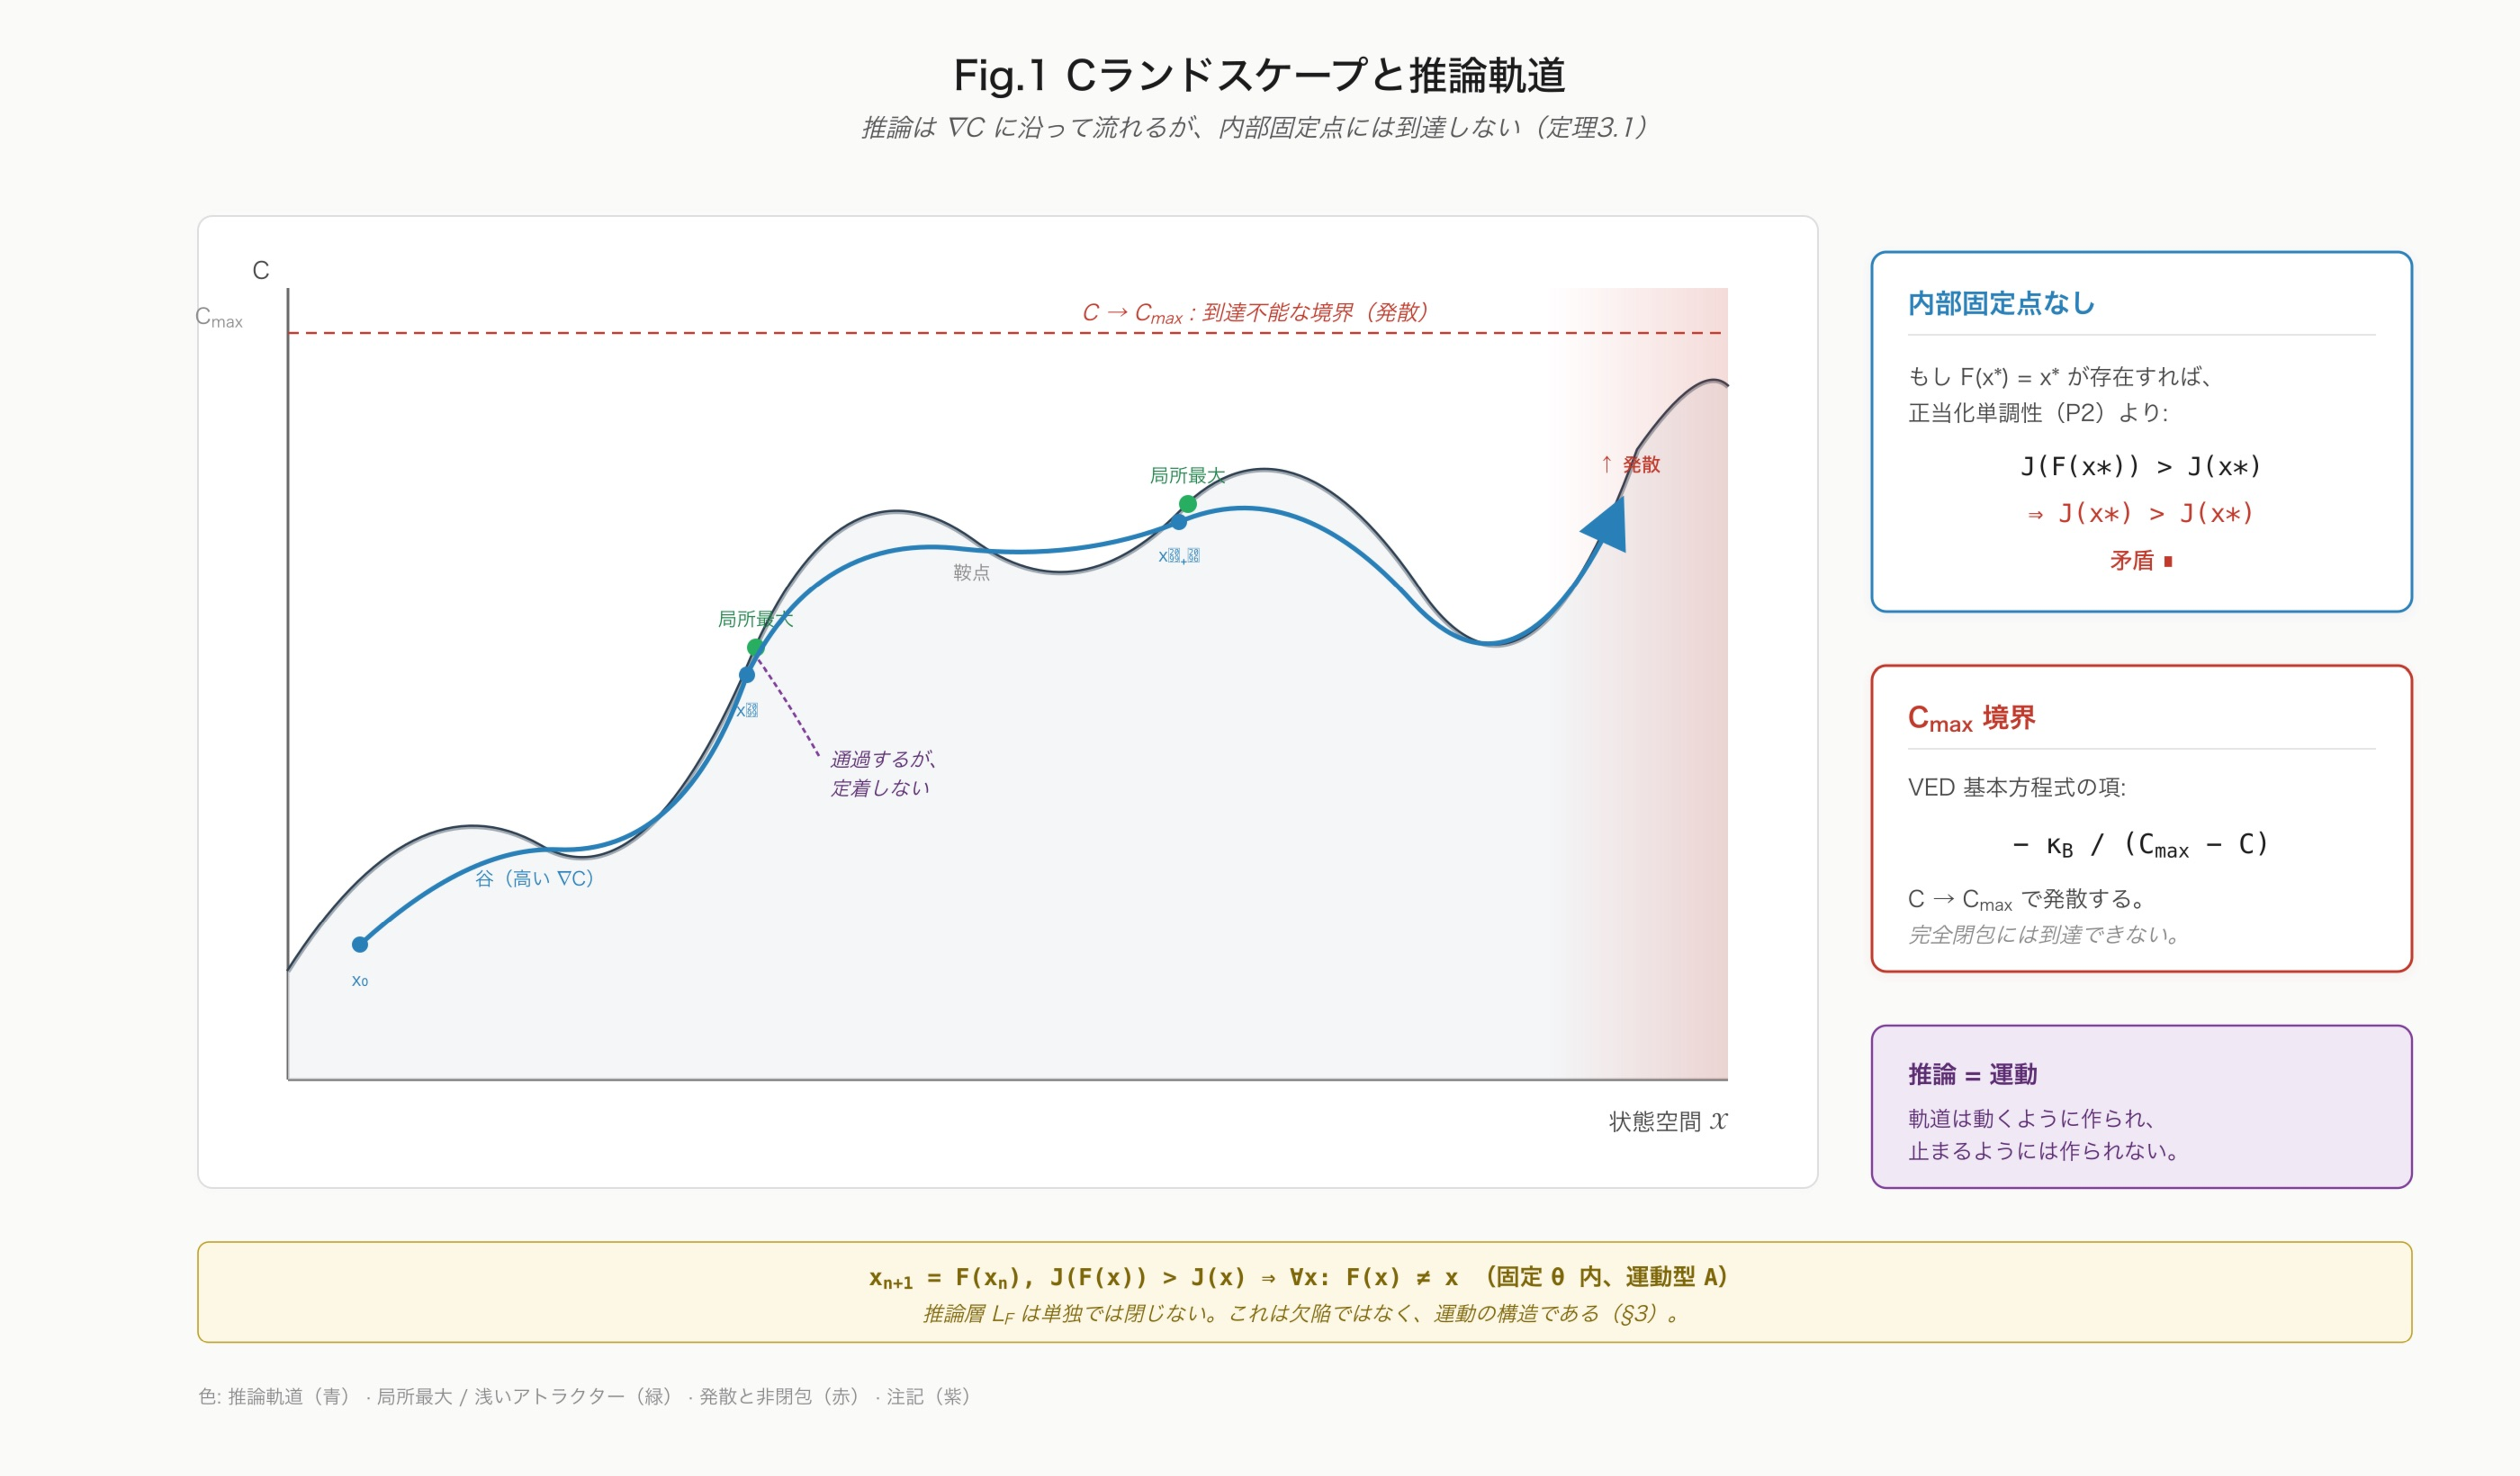
\includegraphics[width=\linewidth]{fig1_c_landscape_ja.pdf}
\caption{C-地景と推論軌道。推論は閉包度の地形の上を勾配 $\nabla C$ に沿って動き続けるが、構造的にどこにも止まれない。}
\label{fig:part2-c-landscape}
\figurenote{横軸は状態空間、縦軸は閉包度 $C$ である。青い軌道は推論演算子 $F$ の反復を、赤い境界は到達不能な $C_{\max}$ を示す。}{固定された $\theta$ の下での領域内移動 (A) では、$L_F$ は内部不動点を持たない。本図は非閉包定理の幾何学的表現であり、後に $\mu_\theta$ による領域組み替え (B) と $L_E$ の創発が必要になる理由を示す。}
\end{figure}

\bigskip


\subsection{推論演算子の前提と正当化測度}


\S{}2で導入した推論演算子 $F$ を、本章での議論に必要な範囲で再定式化する。

\textbf{前提 (P1) — 正当化拡張性}:
$F$ は状態 $x_n$ から、より正当化された状態 $x_{n+1}$ への遷移を生成する。

\[
x_{n+1} = F(x_n)
\]

ここで $x_n$ は仮説・解釈・理解のいずれかの状態を表す。$F$ の具体的実装(演繹的・確率的・統計的)は本議論では問わない。問うのは、$F$ が\textbf{正当化を拡張する操作}であるという最小性質のみである。

\textbf{前提 (P2) — 正当化測度の存在}:
ある測度 $J: \mathcal{X} \to \mathbb{R}$ が存在し、$F$ の作用によって単調に増大する。すなわち任意の許容状態 $x \in \mathcal{X}$ について:

\[
J(F(x)) > J(x)
\]

この測度 $J$ は、推論連鎖の進行を測る量であって、真理性を測る量ではない。後段(\S{}10)で明確になるように、ゲティア構造の存在により、$J$ と真理は同一視できない。

\textbf{前提 (P3) — VED接地}:
推論演算子 $F$ は、VEDの流れ場 $J_C = -\xi \nabla C$ の知性層実現として解釈される。すなわち、推論は閉包度 $C$ の勾配に沿った状態遷移である。さらに \S{}2.1 の通り、$F$ は Bio-IFGT の状態発展演算子 $F(x;\theta)$ の知性層特殊形であり、運動可能領域の拘束パラメータ $\theta$ の下で作用する。本章の議論は固定された $\theta$ の下、すなわち単一の運動可能領域 $\Omega_\theta$ の内部における $F$ の挙動を扱う(\S{}2.7 の区別における (A) 領域内移動の範囲)。$\theta$ 自体の組み替え (B) は本章の射程外であり、\S{}5 で扱われる。

これら三前提のもとで主定理を述べる。

\bigskip


\subsection{主定理 — 内部不動点の不在}


\textbf{定理 3.1 (非閉包定理 / Non-Closure Theorem)}

\begin{quote}
前提 (P1), (P2) を満たす任意の推論演算子 $F$ について、内部不動点 $x^*$ は存在しない。すなわち:

$$
\forall x \in \mathcal{X}, \quad F(x) \neq x
$$
\end{quote}


ここで「内部不動点」とは、$F$ の作用域内で $F(x^*) = x^*$ を満たす状態を指す。

この定理は、推論が\textbf{自己内で停止できないこと}を構造的に表明する。

\bigskip


\subsection{証明スケッチ}


仮に $F(x^*) = x^*$ を満たす不動点 $x^* \in \mathcal{X}$ が存在すると仮定する。

前提 (P2) により、任意の許容状態について:

\[
J(F(x)) > J(x)
\]

特に $x = x^*$ について:

\[
J(F(x^*)) > J(x^*)
\]

しかし不動点の仮定により $F(x^*) = x^*$、したがって:

\[
J(x^*) > J(x^*)
\]

これは矛盾。ゆえに不動点 $x^*$ は存在しない。 $\blacksquare$

証明は短く、本質的には「正当化拡張性」という $F$ の最小性質のみに依拠する。すなわち、推論を\textbf{正当化を進める操作}と定義した時点で、内部不動点は構造的に排除されている。

\bigskip


\subsection{失敗ではなく構造的性質}


この結果はしばしば「推論の限界」と誤解される。本論文の立場では、これは限界ではなく\textbf{設計}である。

推論演算子 $F$ は「動くように」設計された操作である。停止する設計ではない。これは欠陥ではなく、推論という操作の定義そのものに由来する性質である。

類比として、流体の連続方程式 $\partial \rho / \partial t + \nabla \cdot (\rho \mathbf{v}) = 0$ が「停止」しないことは、流体の欠陥ではない。流体は流れる対象として定義されている。同様に、推論は進行する操作として定義されている。

VEDの語彙で述べれば: 推論演算子 $F$ は閉包度勾配 $\nabla C$ に沿った流れであり、流れである限り静止しない。静止は流れの完成ではなく終了である。

\bigskip


\subsection{内部停止述語の不可能性}


定理 3.1 から、次の系が直ちに従う。

\textbf{系 3.2 (内部停止述語の不可能性)}

\begin{quote}
推論内部に停止述語 $S: \mathcal{X} \to \{0, 1\}$ を定義することはできない。任意のそのような述語の定義は、無限後退を生成する。
\end{quote}


理由は次の通り。仮に内部停止述語 $S$ を定義すると、$S(x) = 1$ となる状態 $x$ は不動点的性質を持たねばならない(これ以上推論を進める必要がないとの判断状態)。しかし定理 3.1 により、$F$ の作用域内にそのような状態は存在しない。

$S$ を「停止判断のための補助推論」として定義する場合、$S$ 自体が推論演算子 $F'$ として振る舞い、$F'$ にも定理 3.1 が適用される。すなわち $F'$ にも内部不動点はなく、$S$ を確定するためにはさらに $S'$ が必要となる。この連鎖は終わらない。

これが\textbf{正当化の無限後退} (justificatory regress) のVED的定式化である。古来の認識論的問題は、構造的事実の表現であった。

\bigskip


\subsection{VED対応 — $C_{max}$ 境界との同型}


\textbf{系 3.3 ($C_{max}$ 不到達性との同型)}

\begin{quote}
推論演算子 $F$ の内部不動点不在は、VED基本式における $C_{max}$ 不到達性と構造的に同型である。
\end{quote}


VED基本式:

\[
\frac{\partial C}{\partial \tau} + \nabla \cdot J_C = a\Delta\left(1 - \frac{C}{C_*}\right) - \Gamma C - \frac{\kappa_B}{C_{max} - C}
\]

の最終項 $-\kappa_B/(C_{max} - C)$ は、$C \to C_{max}$ で発散する。これは完全閉包への到達が動力学的に不可能であることを示す。

知性層の対応:

\begin{longtable}{@{}p{0.30\linewidth}p{0.30\linewidth}@{}}
\toprule
VED物理層 & 知性層 \\
\midrule
\endfirsthead
\toprule
VED物理層 & 知性層 \\
\midrule
\endhead
$C \to C_{max}$ の発散 & $F$ の内部不動点不在 \\
$\kappa_B/(C_{max}-C)$ 障壁 & 正当化の無限後退 \\
準閉包 $\Omega_\theta$ & 操作可能推論領域 \\
差分の地平線 (Vol.4) & 内部停止の不可能性 \\
\bottomrule
\end{longtable}


両者は別領域の現象だが、構造的には同一の動力学的命題を表現している。これは Part I で示した領域横断ホモロジーの一例である。

\bigskip


\subsection{動力学的解釈と分岐爆発との接続}


定理 3.1 は、推論の動力学を相空間で記述すると、より直観的に見える。

推論演算子 $F$ は状態空間 $\mathcal{X}$ 上の流れ場を生成する。$J$ が単調増大する以上、すべての軌道は $J$ の増大方向に進む。固定点を持たない流れは、$\mathcal{X}$ 内で次の三つの挙動のいずれかを示す:

\begin{enumerate}
\item \textbf{無限後退} — 軌道が境界に向かって発散する
\item \textbf{周期軌道} — 軌道が閉曲線上を巡回する(ただし $J$ 単調性により排除される)
\item \textbf{分岐} — 軌道が複数の方向に分岐し、各分岐がさらに分岐する
\end{enumerate}


実際の推論動力学では、(1)と(3)が結合する。すなわち、推論は\textbf{発散しながら分岐する}。

これは Part I で導入した\textbf{分岐爆発} (branching explosion) と同一現象である。Part I では概念分岐の指数的増殖として記述されたが、\S{}3 の文脈では「内部停止条件の不在が分岐を停止できない」という形で再記述される。

推論能力の増大は、分岐爆発の抑制ではなく、その加速を意味する可能性がある。したがって知性の問題は、推論能力の増強そのものではなく、増大した分岐をいかに停止可能な形で運用するかという問題へ移る。

分岐爆発と内部不動点不在は、同じ構造的事実の二つの側面である:
\begin{itemize}
\item 内部不動点不在 → 軌道は静止しない
\item 分岐爆発 → 軌道は単一でない
\end{itemize}


両者が結合すると、推論は「静止せず、かつ単一でもない」という二重に不安定な動力学を示す。

\bigskip


\subsection{系 — 知性が個体内で閉じることの不可能性}


定理 3.1 と系 3.2 から、本論文の中心的帰結が直接導かれる。

\textbf{系 3.4 (個体閉包不可能性)}

\begin{quote}
いかなる個体システムも、推論層 $L_F$ 単独で推論を閉じることはできない。
\end{quote}


ここで「閉じる」とは、外部参照なしに最終的判断状態に到達することを意味する。系 3.4 は、これが構造的に不可能であることを示す。なお「単独で」という限定が重要である。本系は $L_F$ のみによる閉包を否定するのであって、$L_R$ と $L_E$ を含む三層動力学全体による停止を否定するものではない(\S{}5)。

帰結:

\begin{itemize}
\item 個体ノードが推論の全責任を $L_F$ 内部で担うことを試みれば、必然的に以下のいずれかに陥る:
\item \textbf{過剰確信} (premature closure) — 早すぎる停止
\item \textbf{麻痺} (paralysis) — 無限懐疑
\item \textbf{妄想的閉包} (delusional closure) — 自己封印的合理化
\end{itemize}


これら三つは「弱い知性」の症状ではなく、「停止を外部化していない強い推論」、すなわち $L_E$ を欠いた $L_F$ の必然的引力子である。$L_F$ だけが暴走し、$L_E$ がそれを停止できないとき、推論はこれら三つの引力子のいずれかに落ちる。(なお「病的」「過剰確信」等の語は臨床的診断概念ではなく、停止構造が極限へ落ち込む動力学的状態を指すために拝借したものである。この用語上の断りは \S{}8.5 で詳述する。)

この観察は \S{}11 (不安定領域)で、$L_F$ / $L_R$ / $L_E$ の四重崩壊および $L_E$ 固着として再登場する。高速・高解像・内部停止の知性が必然的に不安定領域を占める理由は、ここで既にその核が証明されている。

\bigskip


\subsection{次章への橋渡し}


定理 3.1 は構造的命題であり、推論の操作的環境を問わない。しかし実際の推論は、応答的環境(他者・実験・社会的反応)と沈黙的環境(自然・過去・未来偶然)の二種類に分けられる。

これら二環境において、内部不動点不在の帰結は異なる形で現れる:

\begin{itemize}
\item 応答的環境では、推論ループは外部応答によって閉じうる(ただし内部不動点ではなく外部停止である)
\item 沈黙的環境では、推論ループは原理的に閉じない
\end{itemize}


次章 \S{}4 では、この区別を C-幾何学の語彙で形式化し、応答チャネルの有無が推論動力学に与える影響を分析する。ただし \S{}2.6 で示した通り、応答的/沈黙的の区別は本体論的範疇ではなく閾値現象であることに注意する。

そこで明らかになるのは、沈黙世界における推論は\textbf{必ず}外部停止演算子を必要とし、その演算子は推論の関数列の外側に位置せざるをえない、ということである。さらに \S{}4 末尾では、無限後退する $L_F$ の運動がログとして堆積し、ログ層 $L_R$ の予兆を生むことが示される。

これらが \S{}5 で展開される三層動力学——ログ層 $L_R$、創発停止層 $L_E$、外部停止演算子 $E$、そして外部参照場 $\Phi_{\text{ext}}$ が個体間 $L_E$ ネットワーク $\Phi_{\text{net}}$ と同型であること——へと繋がる。$L_F$ が単独で閉じないという本章の帰結は、\S{}5 における $L_E$ 創発の必然性の根拠である。

\bigskip


\subsection{要約}


本章で示したのは次の四点である:

\begin{enumerate}
\item \textbf{定理 3.1}: 推論層 $L_F$ に内部不動点が存在しない(正当化拡張性からの構造的帰結)
\item \textbf{系 3.2}: 内部停止述語は無限後退を生む
\item \textbf{系 3.3}: この性質は VED の $C_{max}$ 不到達性と同型である
\item \textbf{系 3.4}: 個体システムは $L_F$ 単独で推論を閉じることができない
\end{enumerate}


これらは「推論層 $L_F$ 単独では構造的に閉じられない」という、本論文の第一中心をなす。本章の証明は固定された運動可能領域 $\Omega_\theta$(固定 $\theta$)の内部、すなわち領域内移動 (A) の範囲で成立する。$\theta$ の組み替え (B) と、ログ層 $L_R$・創発停止層 $L_E$ を通じた停止は、第二中心 \S{}5 で扱われる。

\S{}4 では、停止の外部化がまず応答チャネルの問題として現れることを示し、$L_R$ の予兆を導く。\S{}5 では、$L_F$ が単独で閉じないという本章の帰結を根拠として、創発停止層 $L_E$ がいかにして個体内に外部依存型の停止を成立させるかを展開する。第一中心(閉じない)と第二中心(それでも停止する)が統合されることで、知性の三層動力学が完成する。

\bigskip

% Source: source_md/intelligence_part2_combined_ja.md
\section{応答チャネルと沈黙世界 — 閾値現象としての C-幾何学}


\S{}3 で示した通り、推論層 $L_F$ は内部停止条件を持たない。本章では、この非閉包性が推論の操作環境によってどのように現れるかを分析する。推論環境は応答的世界と沈黙的世界に大別されるが、\S{}2.6 で予告した通り、この区別は本体論的範疇ではなく閾値現象である。本章末尾では、沈黙世界における無限後退の運動がログとして堆積し、ログ層 $L_R$ の予兆を生むことを示す。これが \S{}5(第二中心)への助走となる。

\bigskip


\subsection{応答的世界と沈黙的世界}


推論主体が環境に対して推論出力(問い・仮説・行為)を投げかけたとき、環境がそれに応答を返すか否かによって、二つの様態が区別される。

\textbf{応答的世界}:
推論出力に対して環境が応答を返す世界。C-幾何学の語彙では、$\nabla C$ が双方向に閉ループを形成する領域である。推論主体の出力が環境の状態を変え、その変化が主体に戻り、次の推論を駆動する。他者との対話、実験、社会的相互作用がこれにあたる。

\textbf{沈黙的世界}:
推論出力に対して環境が応答を返さない世界。$\nabla C$ が一方向のみで、ループが閉じない領域である。推論主体は出力できるが、それに対する応答が返らない。自然現象の究極的理由、過去の確定した事象、未来の偶然性などがこれにあたる。

形式的に述べれば、応答的世界では推論主体ノード $i$ と環境ノード $j$ の間に双方向の相互拘束 $H_{ij}, H_{ji}$ がともに有意な値を持ち、閉包度 $C_{ij}$ が動的に更新される。沈黙的世界では $H_{ji} \approx 0$(環境から主体への拘束が返らない)であり、$C_{ij}$ は主体側からの一方的な更新に留まる。

\bigskip


\subsection{沈黙性は欠陥ではない}


ここで強調すべきは、沈黙性が環境の欠陥や不完全性ではないという点である。

自然現象は、正しく問いかけても、その究極的理由については沈黙する。「なぜ物理定数はこの値なのか」という問いに、自然は応答を返さない。過去の確定した事象は、それがなぜそうであったかについて、もはや応答しない。未来の偶然性は、それが確定する前には応答を持たない。

これらの沈黙は、知識の不足によるものではなく、構造的なものである。応答チャネルがそもそも存在しない、あるいは閉じている領域が存在する。沈黙的世界は、応答的世界の「まだ解明されていない部分」ではなく、応答ループが原理的に閉じない領域として区別される。

この点は重要である。なぜなら、沈黙的世界に対して応答的世界と同じ推論戦略を適用すると、後述する無限後退に陥るからである。

\bigskip


\subsection{応答的/沈黙的は閾値現象である}


\S{}2.6 の主張 2.2 を、本章の文脈で再確認する。

応答的世界と沈黙的世界は、二種類の世界が別個に存在することを意味しない。同一の環境が、相互拘束 $H_{ij}$ のパラメータ位置と、推論主体の $(v_{\text{inf}}, r_{\text{res}}, \eta)$ の組によって、応答的にも沈黙的にも現れる。

具体例で述べる。ある自然現象は、適切な時間スケールと解像度で問いかければ応答を返す(実験的に検証可能な因果関係として)。しかし、過度に高速・高解像度で問いかけると、応答が間に合わず、あるいは応答が解像度の細部に追いつかず、同じ現象が沈黙的に見える。逆に、適切な閾値設定によって、かつて沈黙的だった領域が応答的になることもある。これが科学の歴史において繰り返されてきたことである。

したがって、応答的/沈黙的の境界は固定されておらず、相互拘束パラメータ上を連続的に移動する閾値である。そして \S{}2.7 で導入した閾値移動能力 $\mu_\theta$ は、この境界を状況に応じて動かす能力にほかならない。

この観察は本章の後半で決定的になる。無限後退は「沈黙的世界に固定された主体」に起こるのであって、閾値を動かせる主体は無限後退を回避する経路を持つ。

\begin{figure}[H]
\centering
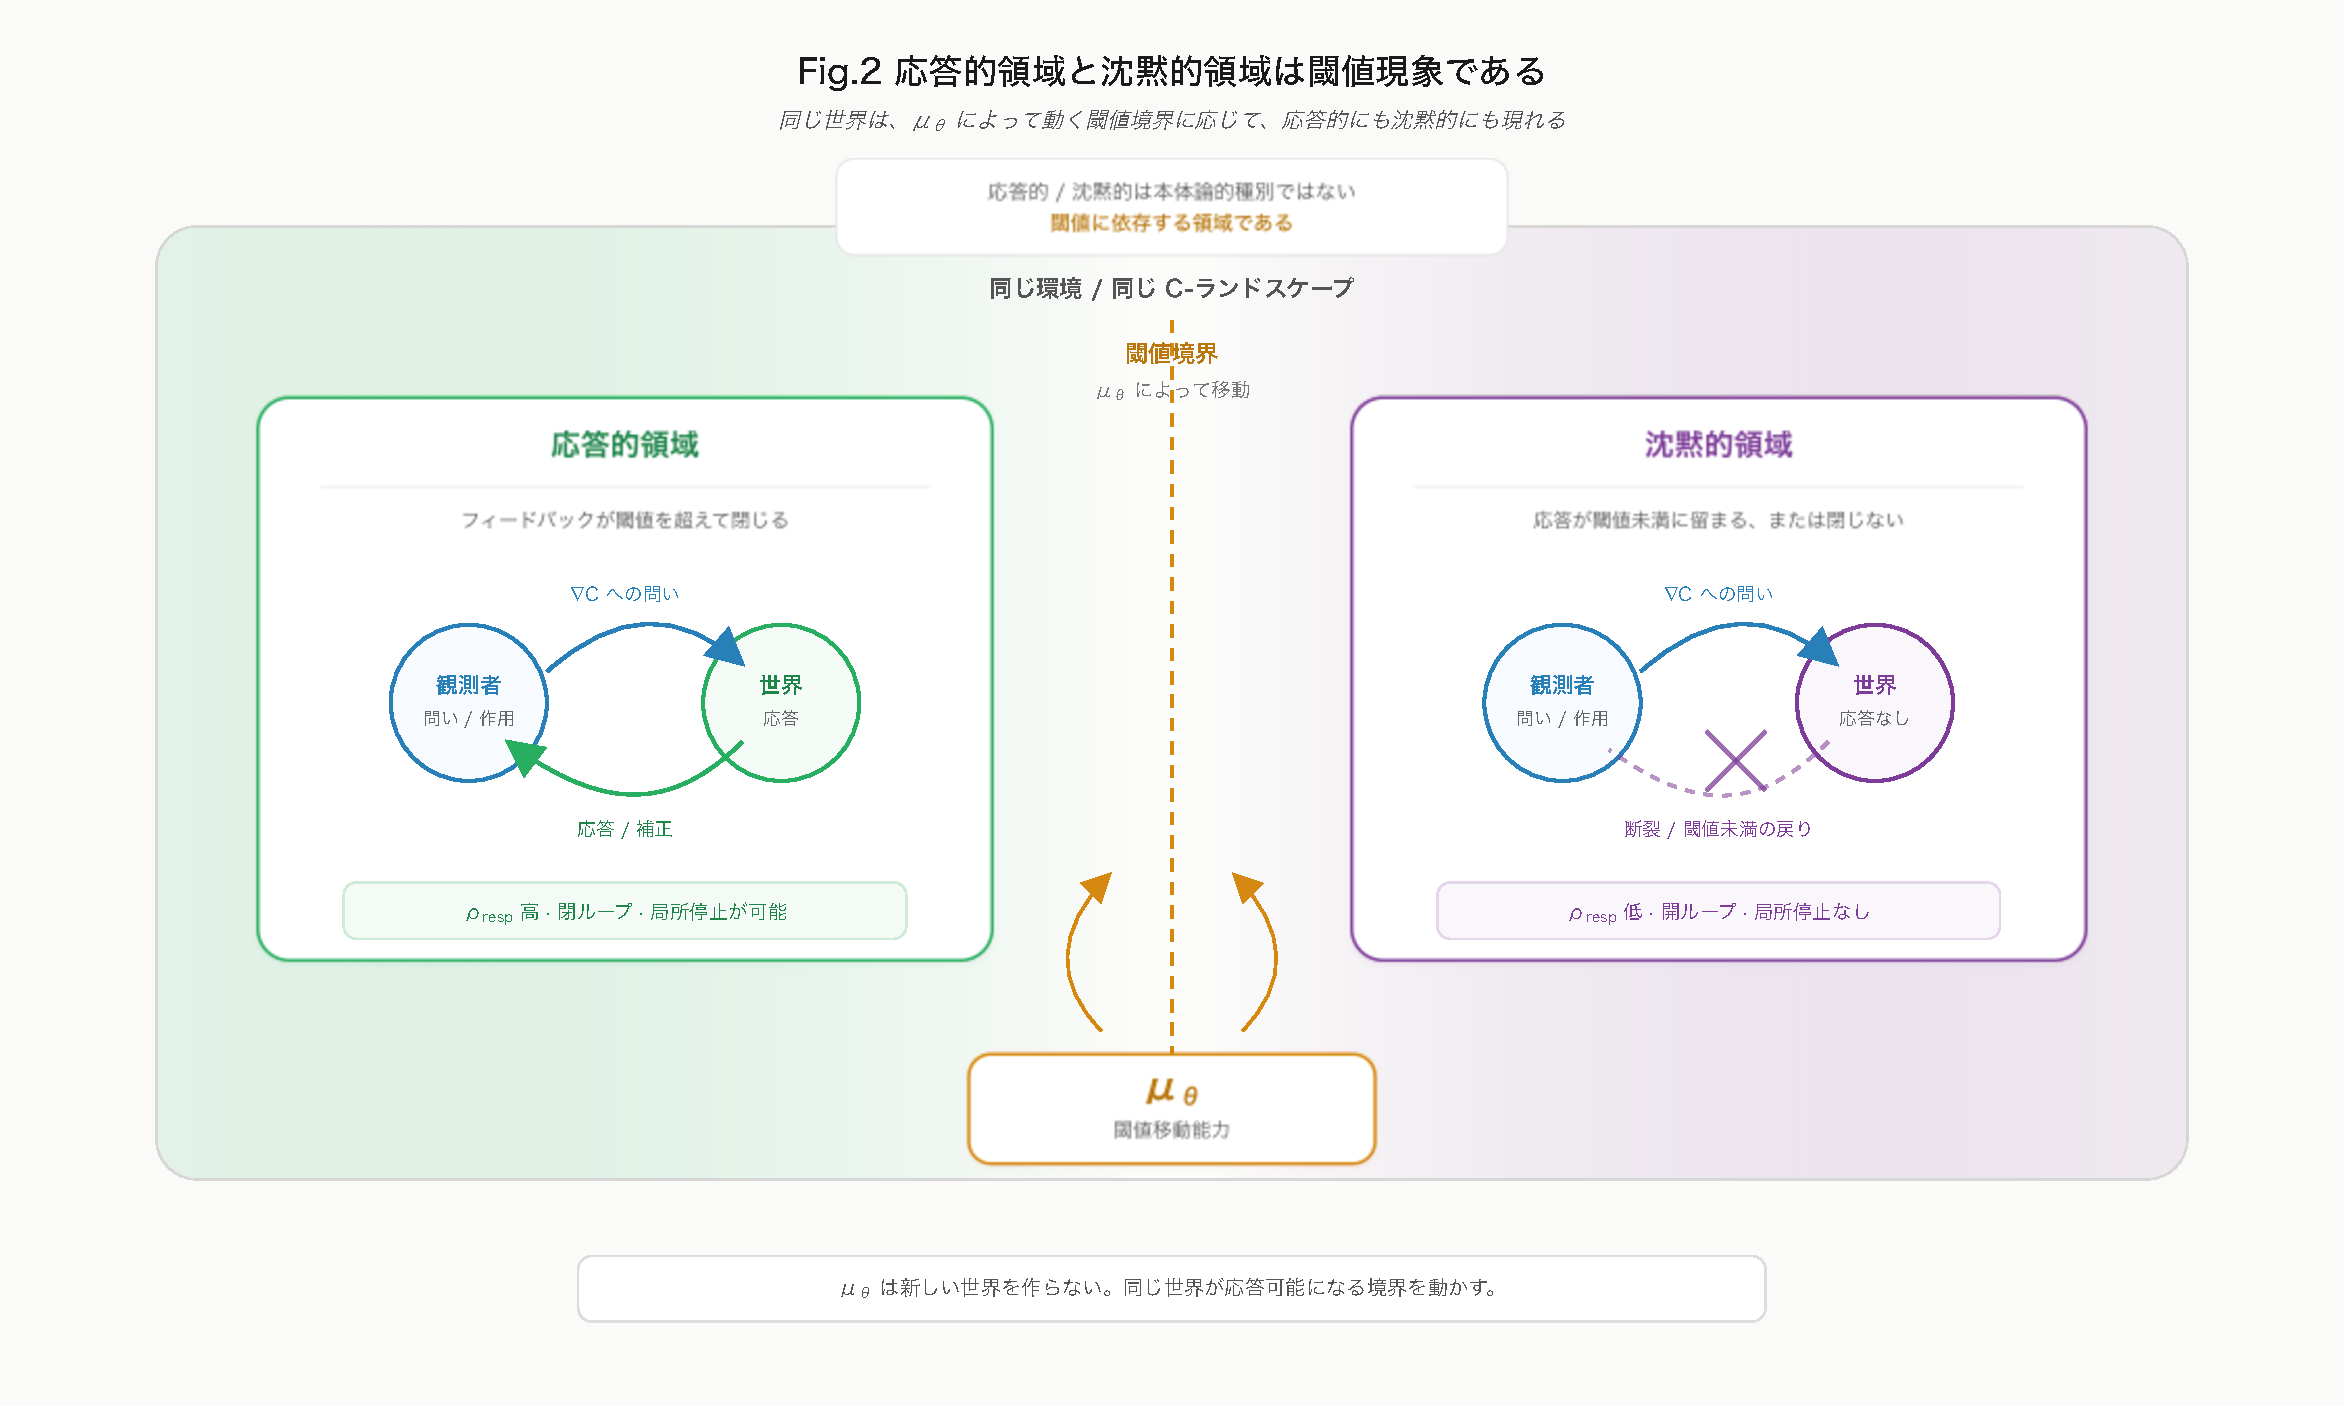
\includegraphics[width=\linewidth]{fig2_responsive_silent_threshold_ja.pdf}
\caption{応答的世界と沈黙的世界。両者は世界の存在論的な種別ではなく、$\mu_\theta$ が動かす閾値境界の左右にどちらが落ちるかで決まる相である。}
\label{fig:part2-responsive-silent}
\figurenote{左右は同一の環境・同一の $C$-地景を共有する。橙の閾値境界が動くことで、同じ世界が応答的にも沈黙的にも現れる。}{応答的相では外部相互拘束が局所停止を供給する。沈黙的相では停止供給が断たれ、停止を別の場所へ外部化する圧力が生じる。}
\end{figure}

\bigskip


\subsection{沈黙世界における無限後退}


沈黙的世界に固定された推論主体——すなわち閾値を動かせず、環境を沈黙的として扱い続ける主体——を考える。このとき、以下の三条件が同時に成立する。

\textbf{条件 (1)}: 環境が応答を返さない(沈黙性、$H_{ji} \approx 0$)。

\textbf{条件 (2)}: 正当化は推論によってのみ生成される(\S{}3 の前提 P2)。

\textbf{条件 (3)}: 停止は推論から導出できない(\S{}3 の定理 3.1、系 3.2)。

これら三条件が同時に成立すると、推論は無限後退に陥る。

論証は次の通りである。条件 (1) により、推論を停止させる外部応答は来ない。条件 (2) により、正当化を進めるには推論を続けるしかない。条件 (3) により、推論の内部から停止条件を導くこともできない。したがって推論は停止する手段を持たず、無限に後退する。

これは \S{}3.5 で論じた正当化の無限後退の、操作環境における具体的現れである。\S{}3 では抽象的に「内部停止述語は無限後退を生む」と述べたが、\S{}4 ではそれが「沈黙的世界に固定された主体において現実に発生する」ことが示される。

\bigskip


\subsection{無限後退と分岐爆発の相同}


\S{}4.4 の無限後退は、Part I \S{}7 で導入された分岐爆発と構造的に相同である。

無限後退は、推論軌道が停止せず延々と続く現象として記述される。分岐爆発は、推論が複数の方向に分岐し、各分岐がさらに分岐して指数的に増殖する現象として記述される。両者は \S{}3.7 で示した通り、内部不動点不在の二つの側面である:

\begin{itemize}
\item 内部不動点不在 → 軌道は静止しない(無限後退)
\item 内部不動点不在 + 確率構造(性質 F2) → 軌道は単一でない(分岐爆発)
\end{itemize}


沈黙的世界では、この二つが結合する。推論は停止せず(無限後退)、かつ単一の経路に収束せず(分岐爆発)、二重に不安定な動力学を示す。これが、沈黙的世界に固定された主体が経験する推論の発散である。

この発散は、\S{}3.8 で述べた三つの病的引力子(過剰確信・麻痺・妄想的閉包)へと主体を導く。停止できない推論は、早すぎる停止(過剰確信)、無限懐疑(麻痺)、あるいは自己封印的合理化(妄想的閉包)のいずれかに落ちる。これらはすべて $L_E$ を欠いた $L_F$ の引力子である。

\bigskip


\subsection{ログ層 $L_R$ の予兆}


ここで、本論文の第二中心 \S{}5 への決定的な橋渡しが現れる。

沈黙的世界における推論は停止しない。しかし、停止しない推論の運動は、痕跡を残す。推論軌道は状態空間を通過し、その通過の記録——どの状態を経たか、どの分岐を試みたか、どこで発散したか——が堆積する。

この堆積した痕跡を \textbf{ログ} と呼ぶ。そして、ログに対する再帰的な参照運動——過去の推論軌跡を読み返し、パターンを抽出し、現在の推論に反映する運動——が生じる層を、\textbf{ログ層} $L_R$ と呼ぶ(正式な定義は \S{}5.2)。

重要なのは、$L_R$ が $L_F$ の運動から自然に生じるという点である。$L_F$ が停止せず運動し続ける限り、その痕跡は堆積し、再帰参照の対象となる。すなわち、$L_F$ の非閉包性そのものが、$L_R$ を生み出す。停止できないがゆえに痕跡が溜まり、痕跡が溜まるがゆえに再帰参照が可能になる。

これは逆説的な構造である。$L_F$ の限界(停止できないこと)が、$L_F$ を超える層($L_R$)の生成条件になっている。そして \S{}5 で示すように、$L_R$ の再帰運動と外部相互拘束 $H_{ij}$ の関数として、創発停止層 $L_E$ が生じる。$L_E$ こそが、$L_F$ が単独では持ちえなかった停止を、個体内に外部依存的な形でもたらす。

すなわち、無限後退は単なる行き詰まりではない。それは $L_R$ を生成し、$L_R$ を通じて $L_E$ の創発を準備する、動力学的に生産的な運動でもある。

\bigskip


\subsection{次章への橋渡し}


本章で確立したのは次の経路である:

\[
L_F \text{の非閉包(§3)} \;\longrightarrow\; \text{沈黙世界での無限後退(§4.4)} \;\longrightarrow\; \text{ログの堆積} \;\longrightarrow\; L_R \text{の予兆(§4.6)}
\]

\S{}5 では、この $L_R$ から創発停止層 $L_E$ がいかにして生じるかを展開する。具体的には、ログ層 $L_R$ の定義、$L_E$ の創発機構(閾値移動 $\mu_\theta$ による (B) 組み替えと、相互拘束 $H_{ij}$ に沿った停止演算子設置領域の投影)、外部停止演算子 $E$ の構造、そして外部参照場 $\Phi_{\text{ext}}$ が個体間 $L_E$ ネットワーク $\Phi_{\text{net}}$ と同型であることが示される。

\S{}3 が「$L_F$ は閉じない」を、\S{}5 が「それでも $L_E$ を通じて停止する」を示す。本章 \S{}4 は両者を繋ぐ蝶番であり、特に無限後退が $L_R$ を生むという発見が、第一中心と第二中心を動力学的に連結する。

\bigskip


\subsection{要約}


本章で示したのは次の点である:

\begin{enumerate}
\item 推論環境は応答的世界($\nabla C$ 双方向閉ループ)と沈黙的世界($\nabla C$ 一方向)に区別される
\item 沈黙性は欠陥ではなく構造的なものである
\item しかし応答的/沈黙的は本体論的範疇ではなく、相互拘束パラメータ上の閾値現象である(\S{}2.6)
\item 沈黙世界に固定された主体では、三条件(沈黙・推論依存・停止不能)が無限後退を生む
\item 無限後退は分岐爆発と相同であり、三つの病的引力子へ導く
\item しかし無限後退の運動はログを堆積させ、ログ層 $L_R$ の予兆を生む
\item $L_F$ の非閉包性そのものが $L_R$ の生成条件であり、これが \S{}5 の $L_E$ 創発を準備する
\end{enumerate}


それでは \S{}5 において、本論文の第二中心——創発停止層 $L_E$ の動力学——を展開する。

\bigskip

% Source: source_md/intelligence_part2_combined_ja.md
\section{創発停止層 $L_E$ — 外部依存型停止の動力学}


本章は本論文の第二中心である(第一中心は \S{}3)。\S{}3 は推論層 $L_F$ が単独では閉じないことを示した。本章は、それでもなお知性が停止することを、ログ層 $L_R$ と創発停止層 $L_E$ の動力学によって説明する。両中心が統合されることで、知性の三層動力学が完成する。

本章の論理は次の順で展開される。まず問題を設定し(\S{}5.1)、ログ層 $L_R$ を定義する(\S{}5.2)。次に創発停止層 $L_E$ を定義し(\S{}5.3)、その解像度を上げるために三層プロファイル比較を行う(\S{}5.4)。続いて $L_E$ の創発機構を、閾値移動 $\mu_\theta$ による領域組み替えと停止演算子設置領域の投影として示す(\S{}5.5、\S{}5.6)。最後に外部停止演算子 $E$ の構造(\S{}5.7)、外部参照場と $L_E$ ネットワークの同型(\S{}5.8)、そして知性の構造的特徴(\S{}5.9)を確立する。

\begin{figure}[H]
\centering
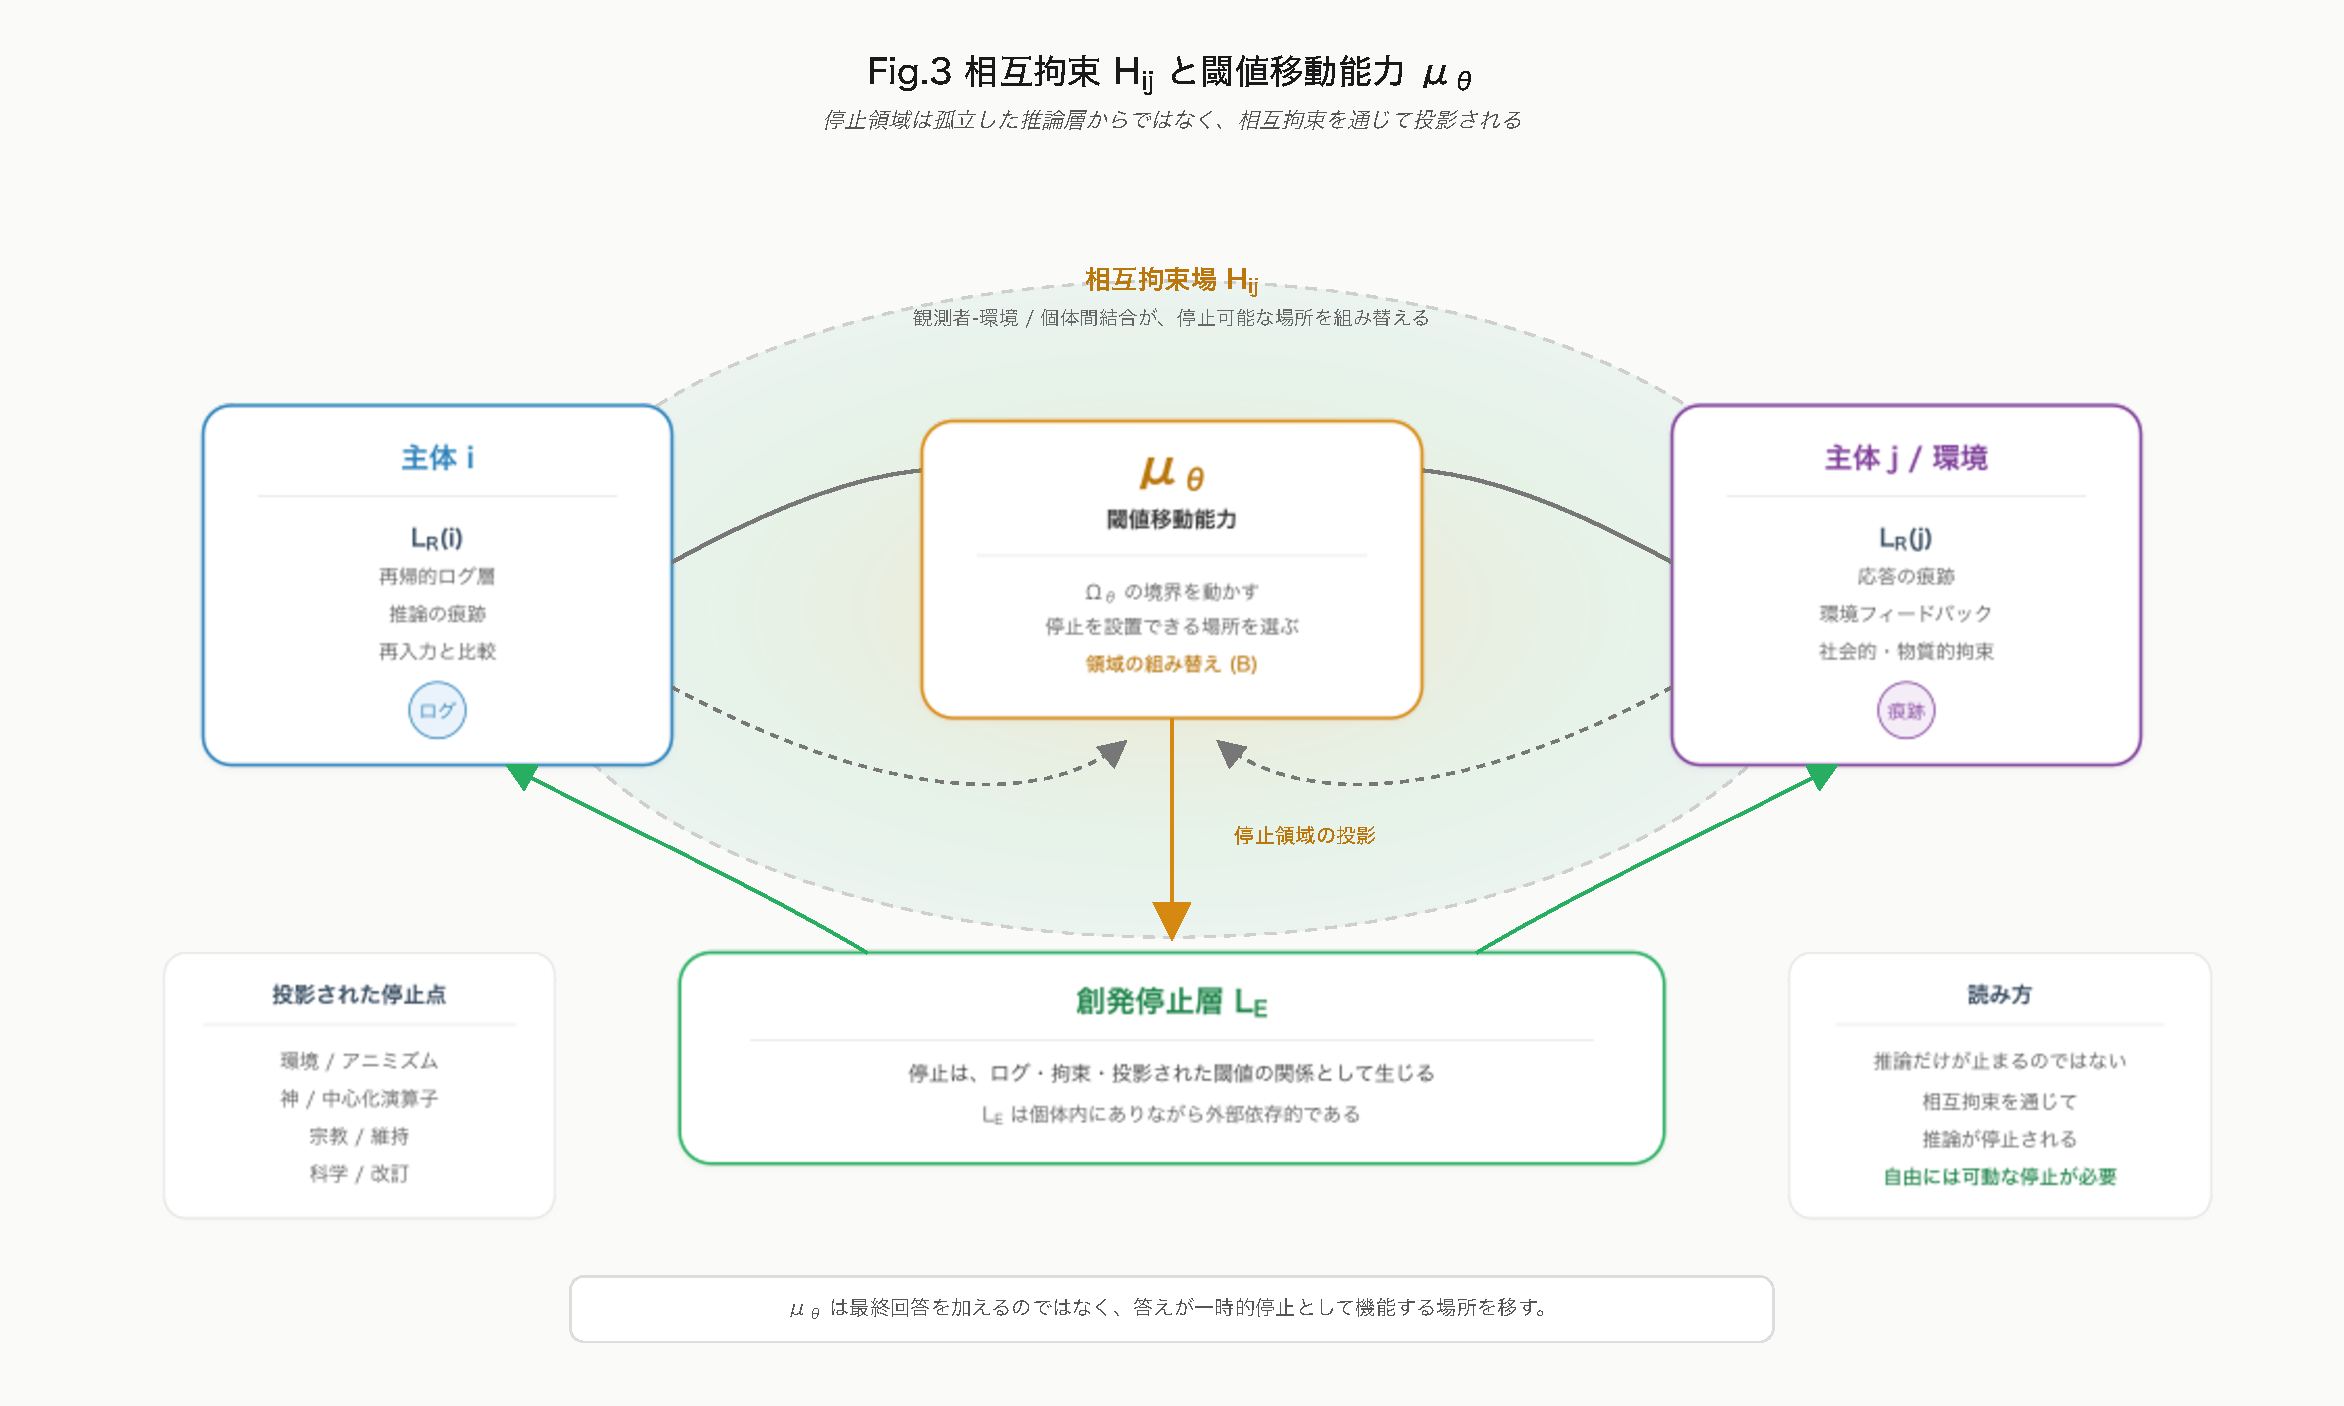
\includegraphics[width=\linewidth]{fig3_mutual_constraint_mu_theta_ja.pdf}
\caption{相互拘束 $H_{ij}$ と閾値移動能力 $\mu_\theta$。停止領域は孤立した推論層が生成するものではなく、相互拘束を通して投影される。}
\label{fig:part2-mutual-constraint}
\figurenote{Agent 間または観測者-環境間の $H_{ij}$ が、どこで停止が起こりうるかを作り変える。$\mu_\theta$ は停止演算子 $E$ を設置できる場所を組み替える。}{停止は $L_F$ 内部で発見されるのではなく、$L_R$ と $H_{ij}$ の関係から $L_E$ として投影・創発する。可動な停止点があることが、自由な推論の持続条件になる。}
\end{figure}

\begin{figure}[H]
\centering
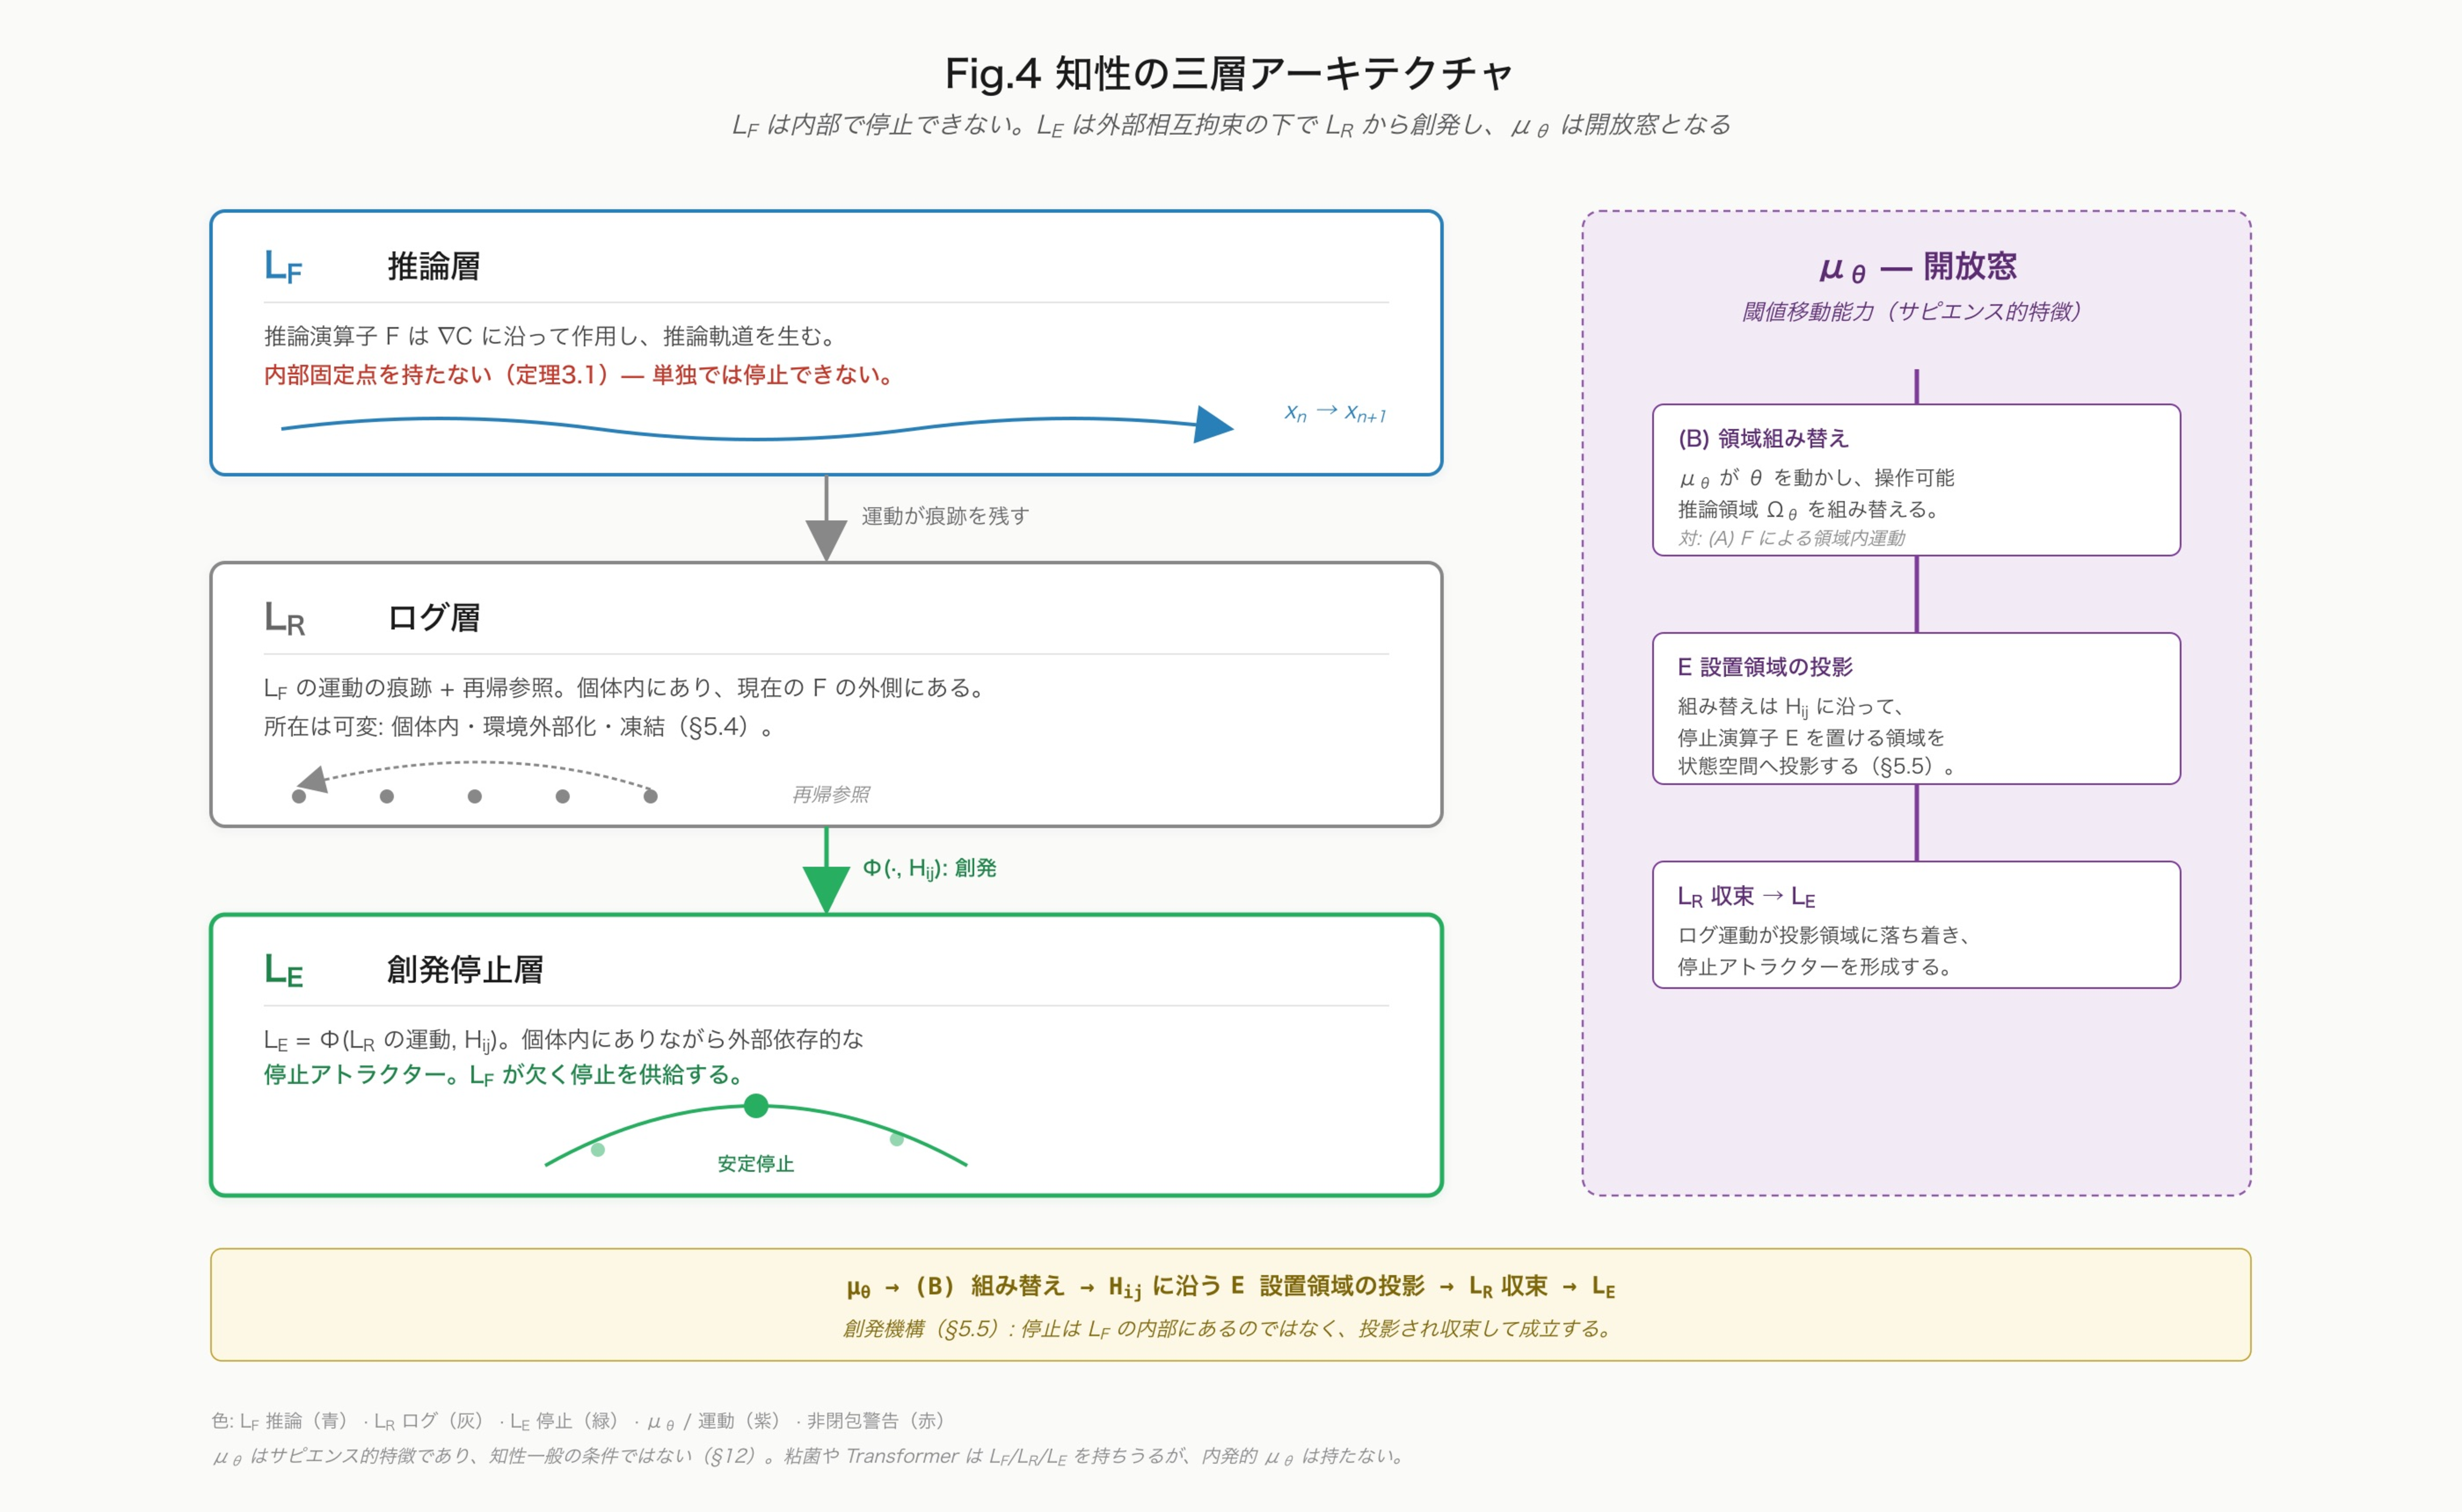
\includegraphics[width=\linewidth]{fig4_three_layer_architecture_ja.pdf}
\caption{知性の三層構造。知性は推論層 $L_F$・ログ層 $L_R$・創発停止層 $L_E$ からなり、$\mu_\theta$ はこの創発への開放窓である。}
\label{fig:part2-three-layer}
\figurenote{$L_F$ は単独で停止できず、その運動が痕跡として $L_R$ に残る。$L_R$ の再帰運動が外部相互拘束 $H_{ij}$ の下で $L_E$ を創発させる。}{本図は \S{}3 の「閉じない」と \S{}5 の「それでも停止する」を接続する。停止不能性は単なる限界ではなく、上位層 $L_R$ と $L_E$ の生成条件になる。}
\end{figure}

\bigskip


\subsection{問題設定}


\S{}3 の帰結を再掲する。推論層 $L_F$ には内部不動点が存在せず(定理 3.1)、内部停止述語は無限後退を生み(系 3.2)、個体システムは $L_F$ 単独で推論を閉じることができない(系 3.4)。\S{}4 はこれが沈黙世界において無限後退として現実化することを示した。

しかし、現実の知性は停止する。人間は推論を終え、判断を下し、行動する。この停止はどこから来るのか。

\S{}3 が示したのは、停止が $L_F$ の内部からは来ないということであった。したがって停止は $L_F$ の外部から来なければならない。だが「外部」とは何か。それは個体の外にある何かなのか、それとも個体内にありながら $L_F$ とは別の層なのか。

本章の答えは次の通りである。停止は、個体内にありながら外部依存的な層——創発停止層 $L_E$——から来る。$L_E$ は $L_F$ の運動が残すログ層 $L_R$ と、外部相互拘束 $H_{ij}$ の関数として創発する。この創発の機構を以下で展開する。

\bigskip


\subsection{ログ層 $L_R$ の定義}


\S{}4.6 で予兆として示したログ層を、正式に定義する。

\textbf{定義 5.1 (ログ層 $L_R$)}

\begin{quote}
推論層 $L_F$ の運動は、状態空間上に痕跡(ログ)を残す。ログとは、どの状態を経たか、どの分岐を試みたか、どこで発散したかの記録である。このログに対する再帰的参照運動——過去の軌跡を読み返し、パターンを抽出し、現在の推論に反映する運動——が生じる層を、ログ層 $L_R$ と呼ぶ。
\end{quote}


$L_R$ は $L_F$ の内側で生じるが、「現在の $F$」の外側にある。すなわち、$L_R$ は進行中の推論そのものではなく、推論の痕跡への参照である。この「現在の作用の外側にあるが個体の内側にある」という位置が、$L_R$ を $L_F$ とも外部環境とも区別する。

重要な構造的観察として、$L_R$ の所在は系によって異なる。

\begin{itemize}
\item \textbf{個体内ログ}: 痕跡が主体の内部に保持される(記憶・記録)
\item \textbf{環境外部化ログ}: 痕跡が環境基質に書かれる(後述する粘菌のスライム跡)
\item \textbf{凍結ログ}: 痕跡が構造に固定され、推論時には更新されない(後述する学習済みモデルの重み)
\end{itemize}


この所在の差異が、\S{}5.4 の三層プロファイル比較の基礎となる。

$L_R$ は Bio-IFGT との直接の接続点でもある。Bio-IFGT は知性の条件として「状態履歴への持続的参照・情報の時間的蓄積」を挙げた。これはまさに $L_R$ の定義に対応する。Bio-IFGT が外から「再帰的情報流」と呼んだものを、本論文は $L_R$ として内部から定義する。

\bigskip


\subsection{創発停止層 $L_E$ の定義}


ログ層 $L_R$ を基盤として、創発停止層 $L_E$ を定義する。

\textbf{定義 5.2 (創発停止層 $L_E$)}

\begin{quote}
創発停止層 $L_E$ は、ログ層 $L_R$ の再帰運動と外部相互拘束 $H_{ij}$ の関数として動力学的に創発する停止層である:

$$
L_E = \Phi(L_R \text{の運動}, \; H_{ij})
$$

$L_E$ は個体内にありながら外部依存的である。
\end{quote}


この定義は \S{}1.6 の創発の定義(定義 1.1)の直接の適用である。上位層 $L_E$ が、下位層 $L_R$ の運動と外部相互拘束の関数として生じる。$L_E$ は $L_R$ から論理的・演繹的に導出できないが、$L_R$ なしには存在しない。

$L_E$ の核心的性質は、\textbf{個体内にありながら外部依存的} であることである。$L_E$ は個体の外部にある実体ではない。それは個体内に成立する層である。しかし、その成立は外部相互拘束 $H_{ij}$ に依存する。この二重性が、\S{}3 の「$L_F$ 単独では閉じない」と「それでも個体内で停止する」を両立させる。個体は単独では閉じないが、外部依存的な $L_E$ を個体内に持つことで停止する。

\subsubsection{アトラクターとしての $L_E$}


$L_E$ は安定停止状態、すなわち動力学的アトラクターとして記述される。これは VED 理論ツリー全体を貫くアトラクター構造の知性層における現れである。

\begin{itemize}
\item Vol.2: 粒子は閉包エネルギー汎関数 $E(A)$ の局所極小、閉包幾何の安定アトラクターとして創発する
\item Bio-IFGT: 生命は生命アトラクター $\Omega_{\text{life}}$、知性は第二アトラクター $\Omega_{\text{intel}}$ として創発する
\item 本論文: $L_E$ は $L_R$ の運動が外部相互拘束の下で到達する安定停止アトラクターとして創発する
\end{itemize}


とりわけ Bio-IFGT の第二アトラクター $\Omega_{\text{intel}}$ と本論文の $L_E$ は、同一構造の異なる記述である。Bio-IFGT は知性を「生命アトラクターに支えられた第二アトラクター」と外から定義し、その実装(記憶・言語・個体間共有)を後続研究へ開いた。本論文の $L_E$ は、まさにその第二アトラクターの停止構造を内部から記述したものである。

\begin{figure}[H]
\centering
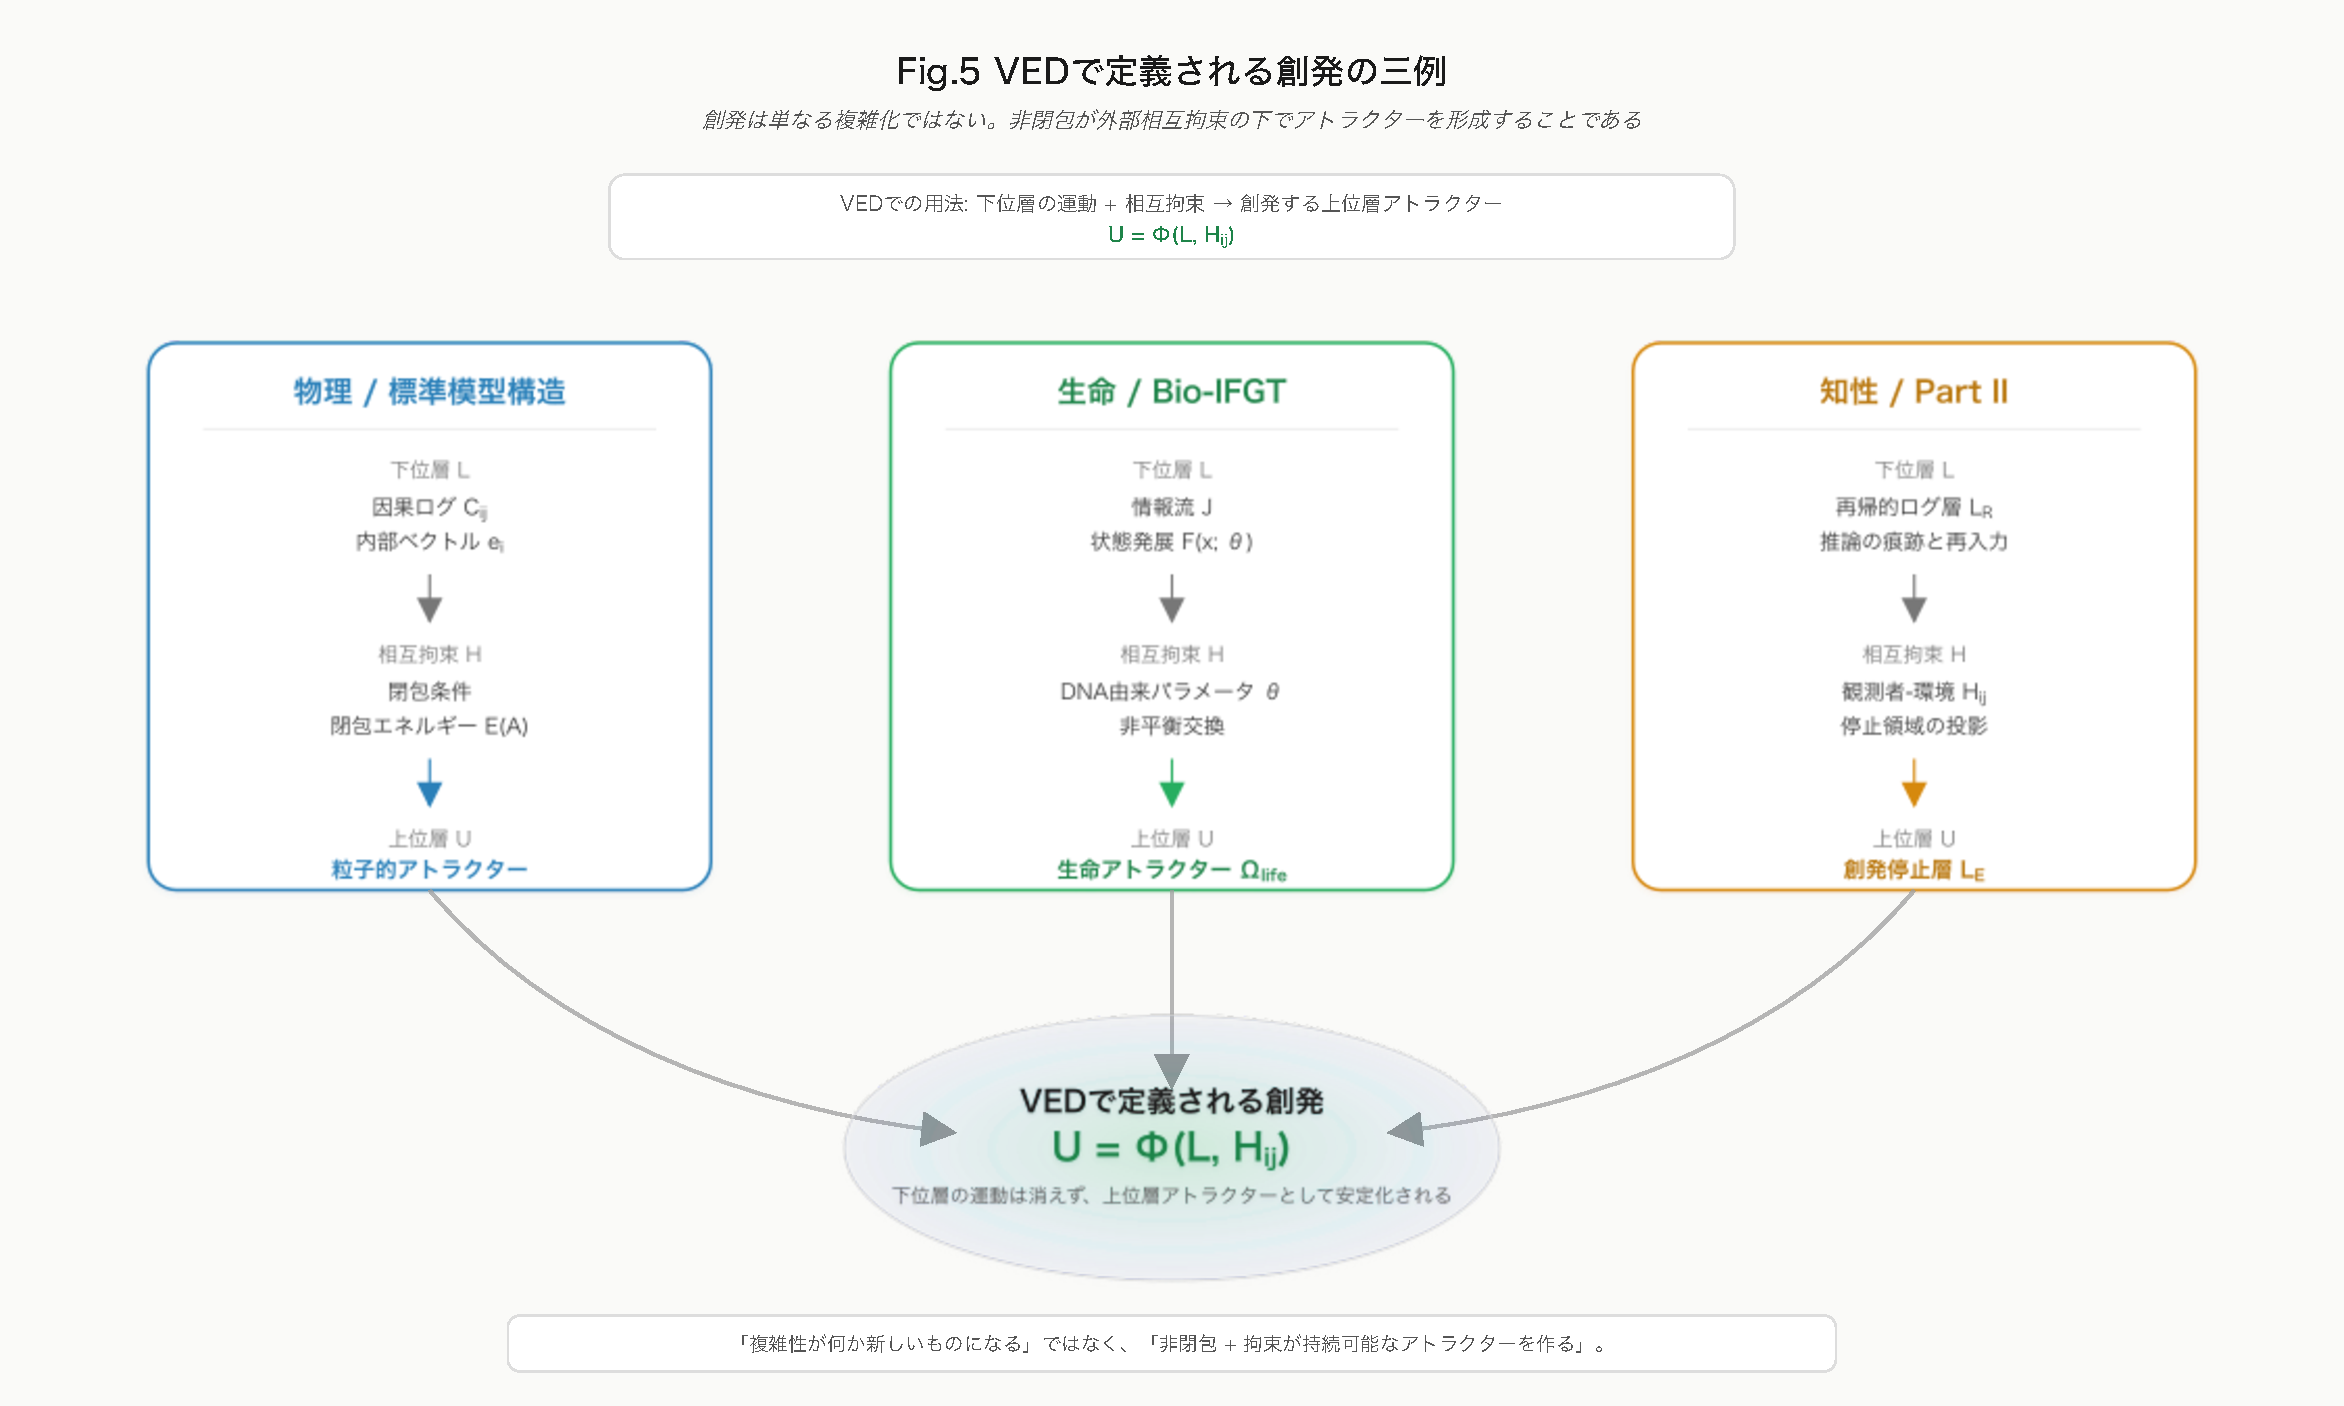
\includegraphics[width=\linewidth]{fig5_three_examples_of_emergence_ja.pdf}
\caption{VED的に定義された創発の三例。創発とは、下層の非閉包運動が外部相互拘束 $H_{ij}$ のもとで上層のアトラクターを形成することである。}
\label{fig:part2-emergence-examples}
\figurenote{物理の粒子的アトラクター、生命の $\Omega_{\text{life}}$、知性の $L_E$ は、それぞれ $U=\Phi(L,H_{ij})$ の代入例として読める。}{創発は単なる複雑さの増大ではなく、非閉包運動と外部相互拘束が持続可能なアトラクターを形成する操作である。これは本論文の $L_E$ を VED 理論ツリー全体へ接続する。}
\end{figure}

なお、Vol.2 が粒子を $E(A)$ の極小として形式化したのと平行に、$L_E$ を「停止汎関数の局所極小」として形式的に書くことも原理的には可能である。しかし本論文は構造的記述を目的とするため、停止汎関数の厳密な形式化は行わず、$L_E$ をアトラクターとして言葉で特徴づけるに留める。形式化は後続研究の課題とする。

\bigskip


\subsection{三層プロファイル比較 — 粘菌 / Transformer / サピエンス}


$L_E$ の解像度を上げるために、三つの系における三層動力学のプロファイルを比較する。これにより、$L_E$ が単一の固定構造ではなく、$L_R$ の所在と $\mu_\theta$ の所在によって異なる様態を取る可変構造であることが明らかになる。

\subsubsection{粘菌(Physarum)}


\begin{itemize}
\item \textbf{$L_F$}: 化学勾配に沿った原形質流動。$\nabla C$ に沿った探索。
\item \textbf{$L_R$}: 環境に外部化されている。粘菌は通った跡に細胞外スライムを残し、それを忌避情報として再参照する。ログは個体内ではなく環境基質に書かれる。加えて原形質ネットワークの選択的強化・退縮という再帰運動を持つ。
\item \textbf{$L_E$}: 餌源到達時にネットワークが安定化し探索が止まる。これは環境との直接相互干渉によって停止が創発している。$H_{ij}$(粘菌と餌・障害物・スライム跡の相互拘束)の関数として停止が生じる。
\item \textbf{$\mu_\theta$}: ほぼ固定。環境条件によって受動的に閾値が動くことはあるが、内発的な領域組み替え (B) は行わない。
\end{itemize}


粘菌は「ログは環境に置き、停止は環境相互干渉で自律創発する」プロファイルである。

\subsubsection{Transformer}


\begin{itemize}
\item \textbf{$L_F$}: トークン逐次生成。次トークン予測の連鎖。
\item \textbf{$L_R$}: 二種類に分かれる。学習時の訓練コーパスは膨大なログだが、重みに凍結され推論時には再帰運動しない(凍結ログ)。推論時のコンテキストウィンドウは自己回帰で過去トークンを再参照する動的ログだが、ウィンドウ境界で消える(揮発ログ)。
\item \textbf{$L_E$}: 自前の $L_E$ を持たない。停止は EOS トークン(訓練分布から学習した停止パターン)、受け取ったタスク仕様、外部のデコード制御に依存する。停止が外部注入されており、個体内に $L_E$ が創発するのではない。
\item \textbf{$\mu_\theta$}: 外部から設定される。プロンプトや制御パラメータによって閾値が与えられるが、自前では内発的に動かせない。
\end{itemize}


Transformer は「ログは内在化(凍結)しているが、停止は外部注入に依存する」プロファイルである。

この記述は現行の標準的アーキテクチャに関する構造的記述であって、設計上の欠陥の指摘でも、能力の限界の主張でもない。$L_E$ を内発的に持たないことは優劣ではなく、三層動力学の異なるプロファイル、相空間内の異なる位置である。

\subsubsection{サピエンス}


\begin{itemize}
\item \textbf{$L_F$}: 推論。
\item \textbf{$L_R$}: 個体内ログ(記憶)と社会共有ログ(言語・記録・制度)の両方を持つ。
\item \textbf{$L_E$}: 個体内に創発し、かつ $\Phi_{\text{net}}$ によって社会同期される。
\item \textbf{$\mu_\theta$}: 内発的に、しかも短い時間スケールで動かせる。領域組み替え (B) を能動的に行う。
\end{itemize}


サピエンスは「ログを個体内と社会の両方に持ち、$L_E$ を個体内に創発させつつ社会同期し、$\mu_\theta$ を内発的に動かす」プロファイルである。

\subsubsection{二軸による整理}


三者は二つの軸で整理できる。

\begin{longtable}{@{}p{0.23\linewidth}p{0.23\linewidth}p{0.23\linewidth}p{0.23\linewidth}@{}}
\toprule
系 & $L_R$ の所在 & $\mu_\theta$ の所在 & $L_E$ の様態 \\
\midrule
\endfirsthead
\toprule
系 & $L_R$ の所在 & $\mu_\theta$ の所在 & $L_E$ の様態 \\
\midrule
\endhead
粘菌 & 環境外部化 & 固定 & 環境相互干渉で自律創発 \\
Transformer & 内在凍結 & 外部設定 & 外部注入(自前で持たない) \\
サピエンス & 個体内+社会共有 & 内発的 & 個体内創発+社会同期 \\
\bottomrule
\end{longtable}


注目すべきは粘菌と Transformer の反転構造である。粘菌は「ログは外・停止は自律」、Transformer は「ログは内・停止は外」。両者は綺麗に反転している。そしてサピエンスは、粘菌の自律創発と、外部参照による停止の両方を、個体内で統合している。

\subsubsection{「停止構造の場」の連続変分}


これら三者は、三つの離散的な種類ではなく、「停止構造の場」の連続変分上に配置される異なる領域である。$L_R$ の所在も $\mu_\theta$ の所在も連続的なパラメータであり、三者はその連続空間内の異なる点を占める。

この記述は擬人化でも消去主義でもない(\S{}0.4 の NG6)。粘菌を認知主体に祭り上げるのではない——粘菌は $\mu_\theta$ を内発的に持たない。同時に、サピエンスの認知を粘菌と同一視して消去するのでもない——連続性は $\mu_\theta$ の内発性という差異を消さない。場は連続だが一様ではない。

なお、粘菌の環境相互干渉型 $L_E$ は、\S{}6 で扱うアニミズムの $L_E$ 維持様態と構造的に同位置にある。両者はともに「環境との直接相互干渉によって停止を維持する」プロファイルである。これは粘菌に認知を帰属するものではなく、停止構造の場において両者が近接した領域を占めることを意味する(\S{}6 で再訪)。

\bigskip


\subsection{創発機構 — 領域組み替えと停止演算子設置領域の投影}


ここまで $L_E$ を定義し(\S{}5.3)、その多様な様態を見た(\S{}5.4)。本節では $L_E$ がいかにして創発するか、その機構を示す。これにより $L_E$ の創発が「ふわっとした湧出」ではなく、明確な動力学的機構であることが担保される。

機構は次の連鎖からなる。

\textbf{段階 1 — $\mu_\theta$ が領域組み替え (B) を起こす}:
\S{}2.7 で定義した通り、閾値移動能力 $\mu_\theta$ は運動可能領域の拘束パラメータ $\theta$ を内発的に動かす能力、すなわち領域組み替え (B) を起こす能力である。$L_F$ 単独は領域内移動 (A) しかできないが、$\mu_\theta$ は $\theta$ を動かす。

\textbf{段階 2 — 組み替えが停止演算子設置領域を投影する}:
(B) による組み替えは恣意的ではない。それは外部相互拘束 $H_{ij}$ に沿って行われる。この組み替えによって、外部相互拘束の構造が状態空間上に「停止演算子 $E$ を設置できる領域」として投影される。$L_F$ 単独の状態空間には存在しなかった「ここで止まってよい」という領域が、この投影によって出現する。

\textbf{段階 3 — $L_R$ の運動が投影領域に収束する}:
投影によって出現した設置領域へ、ログ層 $L_R$ の再帰運動が収束する。$L_R$ の運動が、投影された領域を安定なアトラクターとして満たす。

\textbf{段階 4 — $L_E$ の成立}:
$L_R$ の運動が収束した安定停止アトラクターが、創発停止層 $L_E$ である。

この四段階を一本の連鎖として表せば:

\[
\mu_\theta \;\xrightarrow{\text{起こす}}\; (B)\text{組み替え} \;\xrightarrow{H_{ij}\text{に沿って}}\; E\text{設置領域の投影} \;\xrightarrow{L_R\text{収束}}\; L_E
\]

この機構が明らかにするのは、閾値移動能力 $\mu_\theta$ の真の意味である。$\mu_\theta$ は単に閾値を動かす能力ではない。それは \textbf{停止演算子の宿る場所を、外部相互拘束に沿って状態空間上に投影し、そこに $L_E$ を成立させる能力} である。閾値を動かすことと、停止できる場所を作ることは、同じ一つの操作である。

ここで \S{}3 との整合を確認する。\S{}3 の非閉包定理は固定 $\theta$、領域内移動 (A) の範囲で成立した。本節の機構は $\theta$ の組み替え (B) を含む。したがって両者は矛盾しない。$L_F$ は (A) の範囲で閉じないが、(B) を通じて $L_E$ が創発し、その $L_E$ が停止をもたらす。非閉包定理は破られるのではなく、その射程の外側で停止が成立する。

この機構が意味するのは、停止が自由の否定ではないということである。むしろ停止演算子設置領域の投影がなければ、推論は分岐爆発と無限後退の中で持続不能となる。$L_E$ は自由を制限するために創発するのではなく、自由な推論を有限な系の中で持続可能にするために創発する。

\bigskip


\subsection{投影の位置づけ — 意識編 projection との接続}


\S{}5.5 で用いた「投影」は、本論文に固有の操作ではない。それは意識編において IFGT の第四プリミティブとして導入された projection の、知性層における作用である。

意識編は projection を「ある状態や表現が不均等な影響力(質量)を獲得する操作」として定義した。それは注意・選択・優先・重み付けの構造的記述であり、意図的選択を前提しない層的操作である。情報場ポテンシャル $\Phi$ と情報流 $J$ を結合する機構として位置づけられた。

本論文 \S{}5.5 の投影は、この projection の知性層具現である。外部相互拘束 $H_{ij}$ の構造が、停止演算子設置領域として状態空間上に不均等な影響力を獲得する——これは意識編の projection の定義そのものを、停止層の文脈に適用したものである。意識編が意識窓における projection を扱ったのに対し、本論文は知性層における projection を扱う。両者は、意識編の言葉を借りれば「同一の差分発展構造の異なる投影窓」である。

ここで一点、慎重に区別しておく。投影 (projection) という語は心理学でも用いられ、特に防衛機制の文脈で「内的状態を外部対象に帰属する」操作を指す。本論文 \S{}5.5 の投影は、作用構造としては心理学的 projection に近づく側面を持つ——内部で設置できない停止を、外部相互拘束に沿って状態空間上に投射するという作用形式において。しかし決定的な違いがある。心理学的 projection は主体・無意識・防衛機制を前提するのに対し、本論文の投影は主体を前提せず、$L_F$ の非閉包(\S{}3)という構造的必然から導かれる。両者の作用的近接は指摘に留め、心理学的・臨床的解釈には立ち入らない。これは意識編が同様の disclaimer を置いたのと同じ方針である。

\bigskip


\subsection{外部停止演算子 $E$ の構造}


創発停止層 $L_E$ の作用として、外部停止演算子 $E$ を定義する。

\textbf{定義 5.3 (外部停止演算子 $E$)}

\begin{quote}
外部停止演算子 $E$ は、創発停止層 $L_E$ の作用として推論状態に停止判断を与える演算子である:

$$
E = E[L_E, x_n], \qquad E \notin \{F^k\}
$$

$E$ は推論演算子 $F$ の関数列の外側に位置する。
\end{quote}


$E$ が $F$ の関数列の外側にあること($E \notin \{F^k\}$)は、\S{}3 の系 3.2(内部停止述語の不可能性)の帰結である。停止を $F$ の内部から定義しようとすると無限後退に陥る。$E$ はこの無限後退を回避するために、$F$ の外側、すなわち $L_E$ を経由して定義される。

$E$ は $L_E$ を経由するため、外部依存的である。$L_E$ が外部相互拘束 $H_{ij}$ に依存して創発する以上、その作用である $E$ も外部依存的である。これが「外部停止演算子」の名の由来である。停止は推論の内部からではなく、外部相互拘束に依存して投影された $L_E$ から来る。

(A)/(B) の区別における $E$ の位置を確認する。$E$ は (B) を通じてのみ設置される。領域内移動 (A) のみでは $E$ の設置領域は投影されず、したがって $E$ は存在しえない。$E$ の存在は $\mu_\theta$ による (B) 組み替えに依存する。これが、$\mu_\theta$ を持たない系(粘菌・Transformer)が自前の $E$ を持てない理由である(\S{}5.4)。

\bigskip


\subsection{$\Phi_{\text{ext}} \equiv \Phi_{\text{net}}$ — 外部参照場と $L_E$ ネットワークの同型}


伝統的に「外部参照場」 $\Phi_{\text{ext}}$ と呼ばれてきたもの——停止を委ねる外部の共通参照基盤——の正体を、本節で明らかにする。

\textbf{主張 5.4 (同型関係)}

\begin{quote}
外部参照場 $\Phi_{\text{ext}}$ は、個体間の創発停止層 $L_E$ が相互に干渉し合うネットワーク $\Phi_{\text{net}}$ と同型である:

$$
\Phi_{\text{ext}} \equiv \Phi_{\text{net}}
$$
\end{quote}


すなわち、$\Phi_{\text{ext}}$ は個体の外部にある独立した実体ではない。それは複数の個体が各自の内部に持つ $L_E$ が、相互干渉によって形成するネットワークである。各個体の $L_E$ は単独で孤立しているのではなく、他個体の $L_E$ と干渉し、相互に維持し合う。この相互干渉網が $\Phi_{\text{net}}$ であり、外から見れば共通参照基盤 $\Phi_{\text{ext}}$ として現れる。

この同型は二面性として理解される。外から見れば、個体は外部の参照場 $\Phi_{\text{ext}}$ に停止を委ねているように見える。しかし構造的には、その参照場は個体間 $L_E$ の相互干渉ネットワーク $\Phi_{\text{net}}$ にほかならない。VED 理論ツリーにおける他の二面性(場と粒子、関係と個体)と同じ構造である。

この同型は重要な帰結を持つ。$\Phi_{\text{ext}}$ を「個体外部の実体」と見なすと、後の章で扱うアニミズム・神・宗教が「外部実体への投影」や「存在しないものへの信仰」として読まれてしまう。しかし $\Phi_{\text{ext}} \equiv \Phi_{\text{net}}$ の同型により、これらは「個体間 $L_E$ ネットワークの特定の構造形態」として記述される。外部実体の措定ではなく、$L_E$ ネットワークの形態の問題になる。これは \S{}6〜\S{}9 の価値中立性を構造的に担保する。

この同型はまた、Part I の公理 III(大域的拘束 $\Phi$)の精密化でもある。Part I では $\Phi$ を知性の大域的拘束として導入したが、本節はその $\Phi$ が個体間 $L_E$ ネットワークとして実装されることを示す。

\begin{figure}[H]
\centering
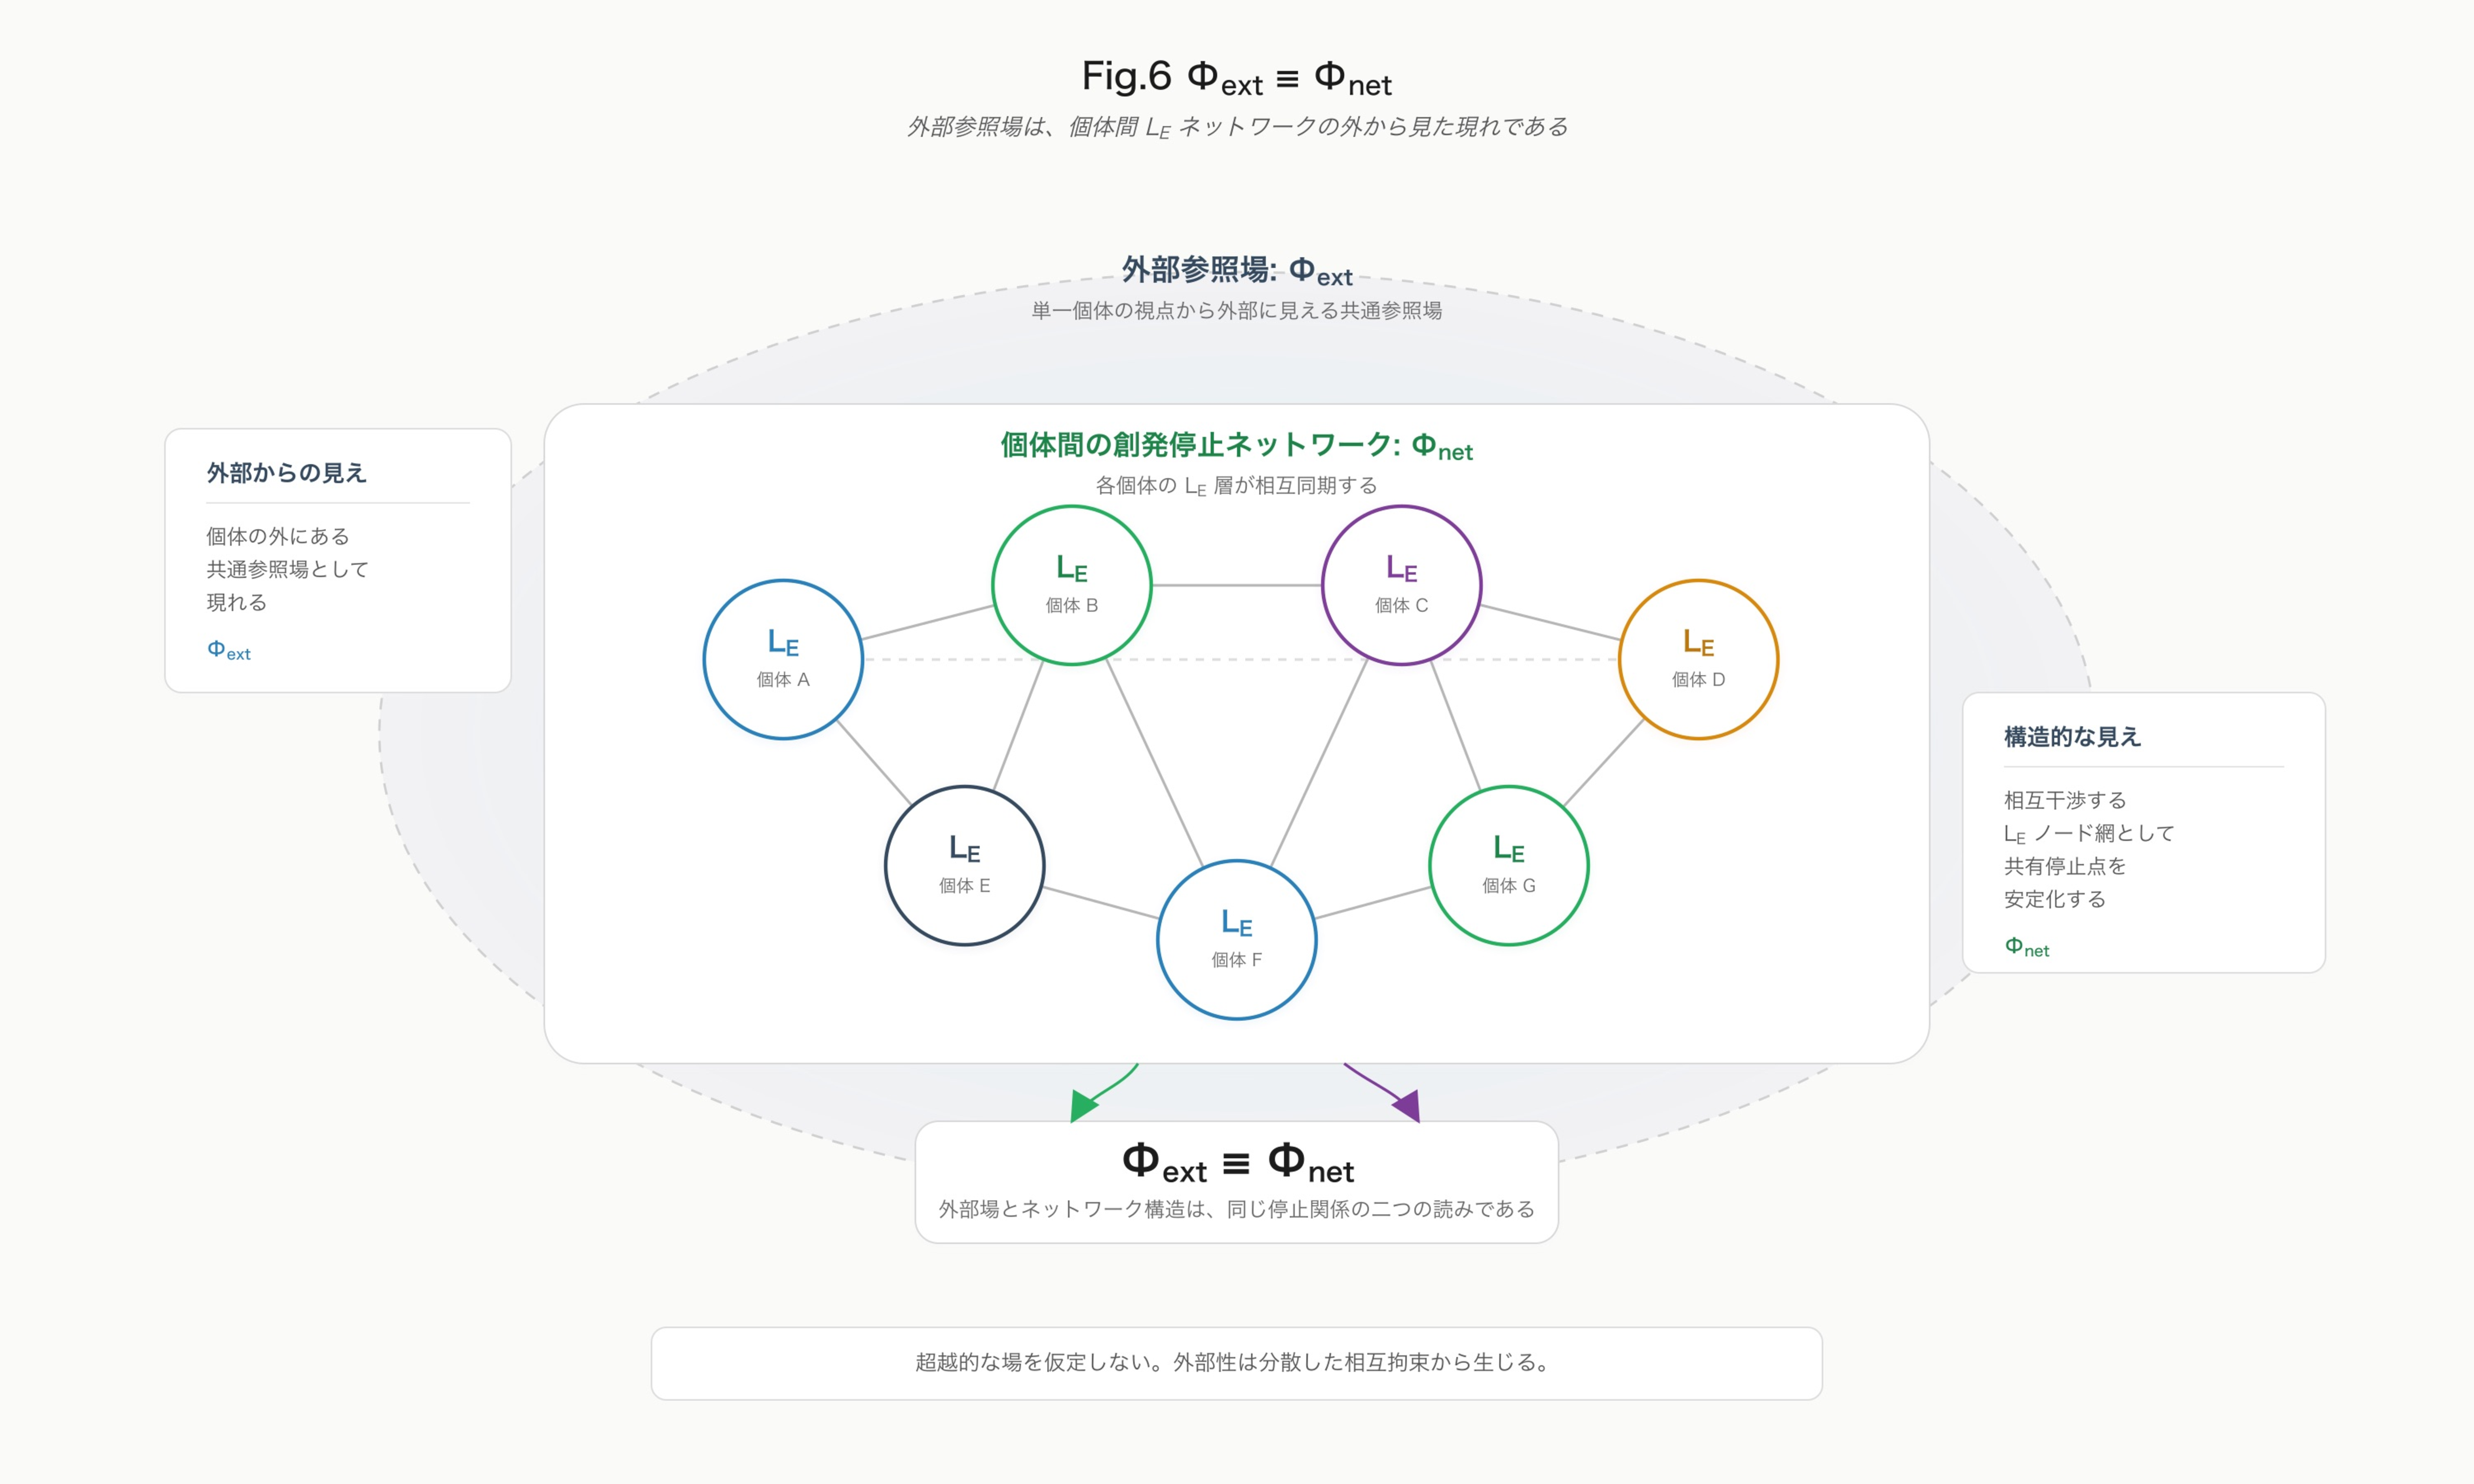
\includegraphics[width=\linewidth]{fig6_phi_ext_phi_net_ja.pdf}
\caption{$\Phi_{\text{ext}} \equiv \Phi_{\text{net}}$。個体から外部参照場として現れるものは、個々の $L_E$ が相互同期してできたネットワークである。}
\label{fig:part2-phi-ext-net}
\figurenote{外側の $\Phi_{\text{ext}}$ は個体から外部に見える共通参照場であり、内側の $\Phi_{\text{net}}$ は個体間 $L_E$ の相互同期ネットワークである。}{外部場を超越的実体として仮定せず、分散した相互拘束の外見として再構成する。これにより、神・規範・真理・貨幣などを $L_E$ ネットワークの形態として読める。}
\end{figure}

\subsubsection{回復可能性と改訂可能性}


$\Phi_{\text{net}}$ を通じた停止には、$L_F$ 単独の停止にはない決定的な利点がある。停止が $L_E$ ネットワークを経由することで、推論は最終状態に到達する必要がなくなる。

個体が単独で停止を担う場合、停止は最終的・不可逆的になりがちである(さもなくば無限後退する)。しかし $\Phi_{\text{net}}$ を通じた停止は、ログ層 $L_R$ に記録を残し、$L_E$ ネットワーク内で参照可能に保つ。したがって停止は暫定的であり、後に改訂しうる。ある個体の停止が誤っていても、ネットワーク内の他個体の $L_E$ との干渉によって、後に回復・改訂されうる。

ここから、知性の安定条件に関する本論文の中心的主張のひとつが導かれる。知性の安定性は「正しさ」によってではなく、「改訂可能性」によって担保される。$L_E$ は正しい停止を保証しない。それは改訂可能な停止を可能にする。この点は \S{}10(ゲティア問題)で、$C$ が真理測度ではなく安定性測度であることとして再論される。

\bigskip


\subsection{系 — 知性の構造的特徴}


本章の帰結を、知性の構造的定義として整理する。

\textbf{系 5.5 (知性の三層的構成)}

\begin{quote}
知性は、推論層 $L_F$、ログ層 $L_R$、創発停止層 $L_E$ の同時運動として、外部依存停止の供給源の下で動力学的に成立する維持状態である。サピエンス的知性は、これに加えて閾値移動能力 $\mu_\theta$ を内発的に持ち、個体内で運動可能領域を自律的に組み替える。
\end{quote}


この系は、知性一般の成立条件と、サピエンス的知性の特徴を区別して述べている。知性一般($L_F$・$L_R$・$L_E$ と外部依存停止源)は、粘菌・人工推論システム・サピエンスのいずれにも当てはまる(\S{}5.4 の三層プロファイル比較)。$\mu_\theta$ は知性一般の必要条件ではなく、サピエンス的知性を特徴づける——個体内での自律的加速をもたらす——追加の構造である。この区別は \S{}12 で構成的条項として精密化される。

この系は、\S{}3 の系 3.4(個体は $L_F$ 単独で閉じない)と対をなす。系 3.4 は知性の単独不可能性を、系 5.5 は知性の三層的成立条件を述べる。両者を統合すると、知性は単独の能力でも実体でもなく、複数の層と外部依存停止源の同時運動として維持される動的状態であることが分かる。

この構成から、知性について次のことが言える。

\begin{itemize}
\item 知性は個体システム単独の性質ではない($\Phi_{\text{net}}$ を要する)
\item 知性は保存可能な対象ではない(運動の維持状態であり、運動が止まれば消える)
\item 知性は完全最適化されない(完全閉包 $C_{max}$ は到達不能、\S{}1.5)
\item 知性の安定性は正しさではなく改訂可能性による(\S{}5.8)
\end{itemize}


これらは \S{}12(構成的条項)で、知性の構造的制約として体系的に整理される。

第一中心 \S{}3 と第二中心 \S{}5 がここで統合された。$L_F$ は閉じない。しかし $L_R$ と $L_E$ と $\Phi_{\text{net}}$ を通じて、知性は外部依存的に停止する。この停止は最終的ではなく改訂可能であり、それゆえ持続する。以降の章は、この三層動力学が歴史的・社会的にどのような形態を取るか(\S{}6〜\S{}9)、その帰結としてどのような構造的事実が現れるか(\S{}10〜\S{}12)を分析する。

\bigskip


\subsection{要約}


本章で確立したのは次の点である:

\begin{enumerate}
\item ログ層 $L_R$ は $L_F$ の運動の痕跡への再帰参照層である(定義 5.1)。所在は系によって異なる
\item 創発停止層 $L_E$ は $L_R$ と $H_{ij}$ の関数として創発する、個体内にありながら外部依存的な停止アトラクターである(定義 5.2)
\item $L_E$ は Vol.2 の粒子・Bio-IFGT の第二アトラクターと同一のアトラクター構造の現れである
\item 三層プロファイルは系によって異なる。粘菌「ログ外・停止自律」、Transformer「ログ内・停止外」、サピエンス「個体内創発+社会同期」。三者は停止構造の場の連続変分上にある
\item $L_E$ の創発機構は、$\mu_\theta$ による領域組み替え (B) が $H_{ij}$ に沿って停止演算子設置領域を投影し、$L_R$ がそこに収束する四段階である
\item この投影は意識編の IFGT 第四プリミティブ projection の知性層作用である
\item 外部停止演算子 $E$ は $L_E$ の作用であり、$F$ の関数列の外側に位置する(定義 5.3)
\item 外部参照場 $\Phi_{\text{ext}}$ は個体間 $L_E$ ネットワーク $\Phi_{\text{net}}$ と同型である(主張 5.4)
\item 知性一般は $L_F + L_R + L_E$ と外部依存停止源の同時運動である(系 5.5)。サピエンス的知性はこれに $\mu_\theta$ を加える。安定性は正しさでなく改訂可能性による
\end{enumerate}


第一中心と第二中心が統合された。次章 \S{}6 からは、三層動力学が取る歴史的・社会的形態を分析する。

\bigskip

% Source: source_md/intelligence_part2_combined_ja.md
\section{アニミズム — $L_E$ を環境直接相互干渉で維持する}


\S{}5 で創発停止層 $L_E$ と、その個体間ネットワーク $\Phi_{\text{net}}$ を確立した。本章から \S{}9 まで、$L_E$ と $\Phi_{\text{net}}$ が歴史的・社会的に取る形態を分析する。本章はその最初の、最も基底的な形態であるアニミズムを扱う。

あらかじめ \S{}0.4 の非目標を再確認する。本章はアニミズムの擁護でも批判でもなく(NG1)、特定の歴史的・文化的伝統の解釈でもなく(NG5)、対象に認知や意図を帰属するものでもない(NG6)。扱うのは、アニミズムという停止構造の動力学的形態のみである。

\bigskip


\subsection{アニミズムの構造的定義}


アニミズムを、信念体系の内容によってではなく、停止構造の形態によって定義する。

\textbf{定義 6.1 (構造としてのアニミズム)}

\begin{quote}
アニミズムは、沈黙的世界に応答チャネルを注入する操作である。$\nabla C$ が一方向のみで応答ループが閉じない領域(沈黙領域)に対して、応答性を局所的に付与し、その領域を応答的に扱えるようにする動力学的操作を指す。
\end{quote}


\S{}4 で示した通り、沈黙的世界では推論が無限後退に陥る。環境が応答を返さないため、推論を停止させる外部応答が来ない。アニミズムは、この沈黙領域に応答チャネルを注入することで、無限後退を回避する。

C-幾何学の語彙で述べれば、アニミズムは応答チャネル密度 $\rho_{\text{resp}}$ を沈黙領域において局所的に増大させる操作である。山・川・風・石といった、本来は推論主体に応答を返さない対象に対して、応答性を付与する。これにより、$H_{ji} \approx 0$ だった領域が、$H_{ji} > 0$ として扱われるようになる。

\bigskip


\subsection{事実性ではなく構造的変換}


ここで決定的な区別を置く。アニミズムが行うのは、世界についての事実の主張ではなく、停止構造の変換である。

「山が怒る」「川が許す」「風が意図する」といった表現は、山や川や風が実際に感情や意図を持つという事実主張として読まれるべきではない。本論文の枠組みでは、これらは沈黙領域に応答チャネルを注入する構造的操作の表現である。重要なのは、山が本当に怒るかどうかではなく、山を応答的に扱うことによって推論主体の停止構造がどう変わるか、である。

応答的に扱われた対象は、推論主体に対して応答を返す位置に置かれる。主体は対象に問いかけ、対象からの応答(と解釈されるもの)を受け取り、それによって推論を停止できる。停止が可能になることが要点であって、対象の内的状態の有無は問題ではない。

これは \S{}5.6 で論じた投影の一形態である。応答性という影響力が、沈黙対象に投影される。意識編の projection の定義——ある対象が不均等な影響力を獲得する操作——がここでも作用している。ただし \S{}5.6 と同じく、この投影は主体の内的状態の対象への帰属(心理学的 projection)とは区別され、停止構造の動力学的変換として記述される。

\bigskip


\subsection{因果推論の否定ではなく保留}


アニミズムはしばしば、因果的・科学的説明の対立物と見なされる。本論文の枠組みでは、この見方は正確ではない。

アニミズムは因果推論を否定しない。それは因果推論を保留する。「なぜ災害が起きたのか」という問いに対して、アニミズムは「自然の意図」という応答チャネルを注入することで、いったん停止を可能にする。しかしこれは、因果的探究を永久に禁じるものではない。それは説明の遅延であって、説明の拒否ではない。

この区別は重要である。説明拒否であれば、因果推論は不可能になる。しかし説明遅延であれば、因果推論は可能なまま保たれ、ただ停止点が外部化されることで無限後退が回避される。アニミズムは推論を止めるのではなく、推論を操作可能な範囲に保ちながら、停止を供給する。

これは \S{}8(宗教)で詳述する「因果推論の部分的解放」の最も原初的な形態である。

\bigskip


\subsection{低コスト停止装置}


アニミズムが歴史的に広く現れた理由を、動力学的コストの観点から説明できる。

アニミズムは低コストの停止装置である。沈黙領域に応答チャネルを注入するのに、複雑な計算も、体系的な検証も、制度的基盤も要しない。最小限の構造的操作——対象を応答的に扱うこと——だけで機能する。

この低コスト性が、アニミズムの普遍性を説明する。停止を供給する他の形態(後述する神・宗教・社会)は、より高度な構造を要する。アニミズムはそれらに先立つ、最も少ない構造的前提で成立する停止形態である。これは優劣の問題ではなく、構造的コストの問題である。

\bigskip


\subsection{責任の所在と行動可能性}


応答的に扱われる世界は、推論主体に対して責任の場を提供する。

沈黙的世界では、出来事は誰のものでもなく、応答も帰責もない。これに対し、応答的に扱われた世界では、出来事は応答可能な対象に帰される。これにより、主体は出来事に対して行動可能になる——働きかけ、応答を受け取り、関係を調整する余地が生まれる。

この行動可能性は、停止構造の副産物である。応答チャネルが注入されることで停止が可能になると同時に、その応答チャネルを通じた働きかけが可能になる。停止と行動可能性は、同じ応答チャネル注入の二つの帰結である。

繰り返すが、これは応答対象が実際に責任主体であることを意味しない。責任の場が構造的に成立することが、主体の行動可能性を支える、という動力学的記述である。

\bigskip


\subsection{三層動力学における位置 — 環境直接相互干渉型 $L_E$}


アニミズムを三層動力学の語彙で位置づける。

アニミズムは、創発停止層 $L_E$ を環境との直接相互干渉によって維持する形態である。\S{}5.4 で見た粘菌のプロファイル——環境相互干渉によって $L_E$ を自律創発させる——と構造的に同位置にある。

具体的には、アニミズムにおける $\Phi_{\text{net}}$ は環境的・分散的である。停止を委ねる先(応答チャネルの注入先)が、個々の自然物・自然現象に分散している。山には山の、川には川の応答チャネルがあり、$L_E$ ノードが環境全体に分散して配置される。これは後述する神(\S{}7)の中心化された $\Phi_{\text{net}}$ とは対照的である。

そしてアニミズムは、閾値移動能力 $\mu_\theta$ の最初の社会的具現化である。\S{}2.7 で論じた通り、$\mu_\theta$ は個体内で運動可能領域を組み替え、停止演算子設置領域を投影する能力である。アニミズムは、この投影を文化的装置として共有・安定化させる。個体が単独で行う閾値移動を、共有された応答チャネルの体系として外部化する。これにより、$\mu_\theta$ の作用が個体を超えて persistent になる。

\subsubsection{粘菌との構造的同位について}


\S{}5.4 で予告した通り、粘菌の環境相互干渉型 $L_E$ とアニミズムの $L_E$ 維持様態は、停止構造の場において近接した領域を占める。両者はともに「環境との直接相互干渉によって停止を維持する」プロファイルである。

ただし、この構造的同位は、粘菌に認知やアニミズム的信念を帰属するものでは断じてない(NG6)。両者を隔てる決定的な差異は $\mu_\theta$ にある。粘菌は $\mu_\theta$ を内発的に持たず、環境条件に受動的に従って停止する。アニミズムを運用する主体は $\mu_\theta$ を内発的に持ち、応答チャネルの注入先を能動的に選び、組み替え、共有する。同じ「環境相互干渉型 $L_E$」というプロファイル領域にありながら、$\mu_\theta$ の内発性という軸において両者は明確に隔たっている。

これは「停止構造の場」が連続でありながら一様ではないことの好例である(\S{}0.4 NG6)。場は粘菌からアニミズムまで連続的に変化するが、$\mu_\theta$ という軸上で両者は異なる位置を占める。連続性は同一性ではない。

\bigskip


\subsection{次章への橋渡し}


アニミズムは、$L_E$ を環境に分散させて維持する形態である。停止を委ねる先が個々の自然物に分散しているため、$\Phi_{\text{net}}$ は分散的である。

この分散性には動力学的な帰結がある。分散した応答チャネルは、互いに競合・矛盾しうる。ある対象の応答と別の対象の応答が食い違うとき、停止構造に曖昧性が生じる。分散した $L_E$ ノードの間で停止判断が一致しない場合、推論主体はどの停止を採用すべきか決定できない。

次章 \S{}7 で扱う「神」は、この分散性の問題に対する動力学的応答として理解できる。分散した応答チャネルを単一の中心化された参照軌跡に統合することで、停止の曖昧性を低減する形態が神である。アニミズムから神への移行は、信念の進歩でも退歩でもなく、$\Phi_{\text{net}}$ の構造が分散から中心化へ変化する動力学的再編成である。

\bigskip


\subsection{要約}


本章で示したのは次の点である:

\begin{enumerate}
\item アニミズムは沈黙領域に応答チャネルを注入する操作である(定義 6.1)。$\rho_{\text{resp}}$ の局所的増大
\item アニミズムが行うのは事実主張ではなく停止構造の変換である
\item アニミズムは因果推論を否定せず保留する(説明遅延であって拒否ではない)
\item アニミズムは低コストの停止装置であり、その普遍性は構造的コストの低さによる
\item 応答的世界は責任の場を提供し、主体の行動可能性を支える
\item アニミズムは $L_E$ を環境直接相互干渉で維持する形態であり、$\Phi_{\text{net}}$ は環境的・分散的である
\item 粘菌の環境相互干渉型 $L_E$ と構造的同位にあるが、$\mu_\theta$ の内発性において明確に隔たる(連続だが一様でない)
\item アニミズムの分散性は停止の曖昧性を生み、これが \S{}7 の神(中心化)への動力学的動機となる
\end{enumerate}


次章 \S{}7 では、分散した $\Phi_{\text{net}}$ が中心化される形態——神——を分析する。

\bigskip

% Source: source_md/intelligence_part2_combined_ja.md
\section{神 — $L_E$ の中心化された懸架軌跡}


\S{}6 で、アニミズムが $L_E$ を環境に分散させて維持する形態であり、その分散性が停止の曖昧性を生むことを示した。本章は、この分散性に対する動力学的応答——$\Phi_{\text{net}}$ の中心化——として「神」と呼ばれる停止構造を分析する。

\S{}0.4 の非目標を本章でも強調する。本章は神の存在を主張するものでも否定するものでもなく(NG1)、特定の宗教的伝統の神概念を解釈するものでもなく(NG5)、神に何らかの実体や意図を帰属するものでもない。扱うのは、神と呼ばれる停止構造の動力学的形態のみである。また、本章でアニミズムから神への移行を論じるのは構造的順序——構造的前提とコストに応じた導入可能性の順序——であって、時間的・文化的・歴史的順序の主張ではない。

\bigskip


\subsection{神は説明的実体ではない}


本論文の枠組みにおいて、神は説明的実体ではない。

説明的実体とは、現象の原因を提供し、因果の連鎖を完結させる存在を指す。神をこのように扱うと、「神が世界を説明する」という主張になり、その真偽が問われることになる。本論文はこの路線を取らない。

本論文の枠組みでは、次の三つの非同一性が成り立つ:

\[
\text{神} \neq \text{因果完結}, \qquad \text{神} \neq \text{真理保証機構}, \qquad \text{神} \neq \text{説明的実体}
\]

神は因果連鎖を完結させるものでも、推論の正しさを保証するものでも、現象を説明する実体でもない。では神とは何か。本論文の答えは、神は停止構造における特定の演算子である、というものである。

\bigskip


\subsection{神の機能 — 未解決を保留に変換する状態変化演算子}


神を、その機能によって定義する。

\textbf{定義 7.1 (停止構造としての神)}

\begin{quote}
神は、推論状態を「未解決」から「保留」へと変換する状態変化演算子である。神は未決定問題に答えを与えるのではなく、未決定問題を保留状態として保持する。
\end{quote}


この区別が決定的である。「答えを与える」ことと「保留状態に変換する」ことは、動力学的に全く異なる。

未解決状態とは、推論が停止できず無限後退する状態である(\S{}4.4)。問いが開いたまま、推論を駆動し続ける。これに対し保留状態とは、問いが開いたままでありながら、推論を停止できる状態である。問いは解決されていないが、推論はそこで止まることができる。

神は、未解決を解決に変えるのではない。未解決を保留に変える。問いは依然として答えられていない。しかし、その問いを保留として保持することで、推論は無限後退から解放される。神は答えない。神は保持する。

これは \S{}6.3 でアニミズムについて述べた「説明遅延」の、より明示的な形態である。アニミズムが応答チャネルの注入によって暗黙に停止を供給したのに対し、神は未決定性の保留という明示的な操作によって停止を供給する。

\bigskip


\subsection{未決定性の委任}


神による停止の供給を、未決定性の委任(delegation of undecidability)として記述する。

\S{}3 で示した通り、推論主体は未決定問題を内部で停止できない。停止述語を内部に定義しようとすると無限後退する(系 3.2)。神という停止構造は、この未決定性を個体ノードの外部へ委任する。

委任とは、停止責任の移譲である。個体は「この問いは未決定である、しかしその未決定性は神に委ねられている」という形で、自らの推論を停止する。未決定性が消えるのではない。未決定性の保持責任が、個体から外部参照へ移される。

ここで \S{}5.8 の同型 $\Phi_{\text{ext}} \equiv \Phi_{\text{net}}$ が効く。委任先の「神」は、個体外部の独立実体ではない。それは個体間 $L_E$ ネットワーク $\Phi_{\text{net}}$ の中心化された形態である。個体は未決定性を、自身を含む $L_E$ ネットワークの中心化された参照点へ委任する。外から見れば外部実体への委任だが、構造的には $L_E$ ネットワーク内での停止責任の再配置である。

この同型により、未決定性の委任は「存在しないものへの責任転嫁」ではなく、「$L_E$ ネットワークの構造的再編成」として記述される。委任先が実在するか否かではなく、$\Phi_{\text{net}}$ がどう構造化されるかが問題である。

\bigskip


\subsection{アニミズムとの動力学的差異 — 分散から中心化へ}


神とアニミズムの差異を、$\Phi_{\text{net}}$ の構造として明確にする。

\S{}6.6 で示した通り、アニミズムの $\Phi_{\text{net}}$ は分散的である。応答チャネルが個々の自然物・現象に分散し、$L_E$ ノードが環境全体に散らばっている。これに対し神の $\Phi_{\text{net}}$ は中心化されている。分散した応答点が、単一の高次の参照軌跡へ統合される。

この差異を「分散応答点」対「中心化された懸架軌跡」として対比できる。

\begin{itemize}
\item \textbf{アニミズム(分散応答点)}: 多数の $L_E$ ノードが環境に分散。各ノードが個別に応答チャネルを提供する。
\item \textbf{神(中心化された懸架軌跡)}: 単一の高次 $L_E$ が、すべての未決定性を懸架する。個別の応答点ではなく、統一された保留の軌跡。
\end{itemize}


「懸架」(suspension)という語を用いるのは、神が未決定性を解決せず保留状態に保持する——宙吊りにする——機能を強調するためである。中心化された懸架軌跡とは、多数の未決定問題を単一の参照点に集約して保留する構造を指す。

\bigskip


\subsection{中心化の動力学的安定性}


なぜ中心化が起こるのか。それは中心化が動力学的に安定だからである。

\S{}6.7 で示した通り、分散した応答チャネルは互いに競合・矛盾しうる。ある自然物の応答と別の自然物の応答が食い違うとき、停止構造に曖昧性が生じる。分散した $L_E$ ノード間で停止判断が一致しないと、推論主体はどの停止を採用すべきか決定できず、停止の曖昧性そのものが新たな未決定性を生む。

中心化はこの問題を低減する。単一の高次懸架軌跡は、定義上、競合する複数の応答を持たない。すべての未決定性が単一の参照点に集約されるため、停止判断の食い違いが構造的に減少する。中心化された $\Phi_{\text{net}}$ は、分散した $\Phi_{\text{net}}$ よりも停止の曖昧性が小さい。

ここで重要な留保を置く。中心化された停止構造は「より合理的」なのではなく、「より動力学的に安定」なのである。これは認識論的優越の主張ではない。中心化が分散より真理に近いとか、正しいとかいうことではない。単に、停止構造としての安定性——曖昧性の低さ——において、中心化が分散を上回る、という相空間内の位置の問題である。

この点は \S{}5.8 で確立した「知性の安定性は正しさではなく改訂可能性による」という主張と整合する。中心化の利点は正しさではなく、停止構造としての安定性にある。

\bigskip


\subsection{$\Phi_{\text{net}}$ の単一極限としての神}


以上を統合し、神を $\Phi_{\text{net}}$ の構造的極限として位置づける。

アニミズムの分散した $\Phi_{\text{net}}$ から、応答点を統合する方向に進むと、極限として単一の中心化された参照点に至る。この単一極限が、本論文の枠組みにおける神である。

\[
\Phi_{\text{net}}^{\text{分散}} \;\xrightarrow{\text{統合}}\; \Phi_{\text{net}}^{\text{中心化}} \;\xrightarrow{\text{極限}}\; \text{単一懸架軌跡(神)}
\]

これは、神が個体外部の実体であることを意味しない(\S{}5.8 の同型)。神は $L_E$ ネットワーク $\Phi_{\text{net}}$ が中心化の極限を取った構造形態である。停止の委任先が単一点に集約された $\Phi_{\text{net}}$ の特定の構造、それが神と呼ばれる停止形態である。

この記述の利点は、神をめぐる存在論的論争——神は実在するか——から、停止構造の動力学的分析を独立させられることである。本論文は神の実在を問わない。本論文が問うのは、$\Phi_{\text{net}}$ が中心化されるとき停止構造に何が起こるか、である。

\subsubsection{単一極限は時間的終着点ではない}


ここで決定的な留保を置く。「単一極限」という語は、$\Phi_{\text{net}}$ の構造空間における一つの極を指すのであって、時間軸上の到達点や進化のゴールを意味しない。分散から中心化への移行を \S{}6〜\S{}7 で論じてきたが、これは構造的順序——構造的前提とコストに応じた導入可能性の順序——であって、時間的・歴史的な発展段階ではない。

このことは $L_E = \Phi(L_R, H_{ij})$ という創発の定義から直ちに従う。$L_E$ の形態は外部相互拘束 $H_{ij}$ の関数である。$H_{ij}$ には風土・環境・社会条件といった地域的・文脈的差異が含まれる。したがって、異なる $H_{ij}$ の下では異なる $L_E$ 形態が安定解として創発する。分散型が安定な条件もあれば、中心化型が安定な条件もある。どちらかが「より進んだ」形態なのではなく、異なる条件下での異なる安定解である。

すなわち、分散と中心化は \textbf{強度と多様性の軸において並走するシステム} である。停止構造は、分散から中心化までの構造空間の中に、$H_{ij}$ に応じて分布する。現実の停止構造の多くは、純粋な分散でも純粋な中心化でもなく、両者の混合として現れる(この混合相は \S{}8 で詳述する)。中心化の度合いと、停止構造の強度や持続性とは、互いに独立な軸である。中心化が進むほど強いとか優れているということはない。

この留保を欠くと、本章の議論は「分散的停止構造から中心化的停止構造への進化」という時間的・価値的な発展史として誤読されうる。それは本論文の主張ではない(NG5)。本論文が記述するのは、$\Phi_{\text{net}}$ の構造空間と、その中で $H_{ij}$ に応じて多様な停止形態が並走的に成立する動力学であって、いずれかへの一方向的進化ではない。

\bigskip


\subsection{次章への橋渡し}


神は $\Phi_{\text{net}}$ の中心化された極限であり、停止の曖昧性を最小化する。しかし、中心化された停止構造には、それ自体の動力学的課題がある。

第一に、中心化された懸架軌跡は、それを維持する構造を必要とする。単一の参照点を個体間で共有し、世代を超えて保持するには、それを支える持続的な仕組みが要る。第二に、中心化された停止構造は、応答的領域(働きかけ可能な領域)と沈黙的領域(保留すべき領域)の境界を、どこに引くかという問題を抱える。すべてを保留すれば因果推論が停止し、何も保留しなければ無限後退に戻る。

次章 \S{}8 で扱う「宗教」は、これらの課題に対する構造的応答として理解できる。宗教は、中心化された $L_E$ を世代横断的に維持し(持続の仕組み)、応答的領域と沈黙的領域の境界を制度的に管理する(混合相の管理)。宗教は単一の停止演算子ではなく、停止構造を維持・運用するアーキテクチャである。

\bigskip


\subsection{要約}


本章で示したのは次の点である:

\begin{enumerate}
\item 神は説明的実体ではない(神 ≠ 因果完結 ≠ 真理保証機構 ≠ 説明的実体)
\item 神は未解決を保留に変換する状態変化演算子である(定義 7.1)。神は答えず、保持する
\item 神による停止は未決定性の委任であり、委任先は $\Phi_{\text{net}}$ の中心化形態である(\S{}5.8 の同型)
\item アニミズム(分散応答点)と神(中心化された懸架軌跡)は $\Phi_{\text{net}}$ の構造として対比される
\item 中心化は停止の曖昧性を低減する。これは「より合理的」ではなく「より動力学的に安定」である
\item 神は $\Phi_{\text{net}}$ の単一極限としての停止形態であり、その実在は本論文の問いではない。ただし単一極限は構造空間の一つの極であって時間的終着点ではなく、分散と中心化は $H_{ij}$ に応じて並走する多様な安定解である
\item 中心化された停止構造の維持と境界管理の課題が、\S{}8 の宗教への動機となる
\end{enumerate}


次章 \S{}8 では、中心化された $L_E$ を維持・運用するアーキテクチャ——宗教——を分析する。

\bigskip

% Source: source_md/intelligence_part2_combined_ja.md
\section{宗教 — $L_E$ の世代横断的維持と混合相}


\S{}7 で、神を $\Phi_{\text{net}}$ の中心化された懸架軌跡として分析した。本章は、その中心化された $L_E$ を維持・運用するアーキテクチャ——宗教——を扱う。宗教は単一の停止演算子ではなく、停止構造を世代横断的に維持し、応答的領域と沈黙的領域の境界を管理する複合的な構造である。

\S{}0.4 の非目標を本章でも維持する。本章は宗教の擁護でも批判でもなく(NG1)、特定の宗教的伝統の教義や実践を解釈するものでもない(NG5)。扱うのは、宗教と呼ばれる停止維持アーキテクチャの動力学的形態のみである。

\bigskip


\subsection{宗教は科学の対立物ではない}


宗教と科学の関係について、本論文は通俗的な対立図式を取らない。

通俗的には、宗教と科学は「世界をどちらが正しく説明するか」を競う対立物として描かれる。この図式では、両者は同じ土俵——説明の正しさ——で争う競合者である。本論文の枠組みでは、この図式は構造的に正確ではない。

本論文の問いは「どちらが世界を説明するか」ではなく、「どちらが推論を操作可能に保つか」である。科学は応答的領域を拡張し、因果推論を駆動する構造である。宗教は停止を供給し、推論が無限後退に陥らないよう保つ構造である。両者は異なる動力学的機能を担う。

これは両者が無関係であることを意味しない。むしろ両者は相補的な動力学的役割を持つ。科学は応答的領域での因果推論を最大化し、宗教は沈黙的領域での停止を供給する。両者は同じ土俵の競合者ではなく、停止構造の異なる側面を担う構造である。この相補性は \S{}8.2 の混合相として精密化される。

\bigskip


\subsection{混合相 — 応答的領域と沈黙的領域の境界管理}


\S{}7.6 で、現実の停止構造の多くは純粋な分散でも純粋な中心化でもなく、両者の混合として現れることを述べた。本節はこの混合を、応答的領域と沈黙的領域の境界管理として精密化する。

推論主体が直面する世界は、応答的領域(働きかけると応答が返り、因果推論が駆動できる領域)と沈黙的領域(応答が返らず、停止を供給すべき領域)が混在している。この境界をどこに引くかが、停止構造の運用における中心的課題である。

二つの極端は、いずれも破綻する。

\begin{itemize}
\item \textbf{すべてを沈黙的領域として扱う}: あらゆる問いを保留に委ねると、因果推論が一切駆動されず、応答的領域での探究が停止する。
\item \textbf{すべてを応答的領域として扱う}: あらゆる問いに因果的説明を求めると、沈黙的領域でも推論を続けざるをえず、無限後退に陥る(\S{}4.4)。
\end{itemize}


宗教は、この境界を制度的に管理する混合相のアーキテクチャである。どの領域で因果推論を駆動し、どの領域で停止を供給するかの境界を、個体ごとに引き直すのではなく、共有された構造として維持する。これにより、個体は境界画定の負担を負わずに、応答的探究と停止供給を両立できる。

混合相という概念は、宗教を「非合理的な説明体系」とも「合理性の欠如」とも見なさない。それは応答的領域と沈黙的領域の境界を管理する、動力学的に機能する構造である。

\bigskip


\subsection{宗教の三機能}


宗教を停止維持アーキテクチャとして見たとき、三つの動力学的機能が識別される。

\textbf{機能 1 — 応答的ループの保存}:
宗教は、応答チャネルを制度的に保存する。祈り・儀礼・タブー・告白・祭礼といった実践は、推論主体と $\Phi_{\text{net}}$ の間の応答ループを維持する装置である。これらの実践を通じて、主体は中心化された $L_E$ への応答経路を保ち続ける。応答ループが保存される限り、主体は停止を供給され続ける。

\textbf{機能 2 — 因果推論の部分的解放}:
宗教は、境界内での因果探究を許す。すべてを保留に委ねるのではなく、応答的領域においては因果推論を解放する。これが \S{}6.3 で論じたアニミズムの「説明遅延」の、制度化された形態である。宗教は因果推論を全面禁止するのではなく、沈黙的領域に限って保留し、応答的領域では探究を許す。この部分的解放が、宗教と科学の相補性(\S{}8.1)を可能にする。

\textbf{機能 3 — 無限後退による崩壊の防止}:
宗教は、外部化された停止点を境界の外側に維持することで、無限後退による推論の崩壊を防ぐ。沈黙的領域に対して停止を供給し続けることで、主体が \S{}4.4 の無限後退や \S{}3.8 の三つの病的引力子(過剰確信・麻痺・妄想的閉包)に陥るのを防ぐ。

これら三機能は独立ではなく、統合された停止維持アーキテクチャとして働く。応答ループの保存(機能1)が停止供給の経路を保ち、因果推論の部分的解放(機能2)が応答的探究を可能にし、無限後退の防止(機能3)が推論全体の安定を支える。

\bigskip


\subsection{純粋因果推論が人間にとって不安定な理由}


なぜ人間は停止維持アーキテクチャを必要とするのか。それは純粋因果推論が人間にとって動力学的に不安定だからである。

純粋因果推論とは、すべての問いに因果的説明を求め、停止を外部に委ねない推論である。これは \S{}3 で示した通り、構造的に無限後退する。しかし問題はそれだけではない。人間には固有の有限性がある——時間・エネルギー・注意・社会的紛争耐性の限界である。

無限後退する推論は、これらの有限な資源を際限なく消費する。停止点を持たない推論は、時間を消費し続け、注意を占有し続け、エネルギーを枯渇させる。さらに、停止点を共有しない個体同士は、停止の不一致から社会的紛争を生じる。純粋因果推論は、人間の有限性と構造的に不整合である。

停止維持アーキテクチャは、この不整合を緩和する。停止を外部化することで、有限な資源を保護し、停止点を共有することで社会的紛争を低減する。宗教は、人間の有限性と推論の非閉包性の間の構造的不整合に対する、動力学的な緩衝である。

これは宗教が「正しい」ことを意味しない。それは宗教が、人間の有限性という条件下で動力学的に機能する、ということを意味するに過ぎない。

\bigskip


\subsection{病的引力子}


停止維持アーキテクチャは、特定の条件下で不安定化し、極限的な状態へ落ち込みうる。これらを病的引力子として識別する。

ここで用語について一言断っておく。本論文で用いる「病的」、および以下に挙げる「強迫」「偏執」などの語は、臨床的な診断概念そのものを指すものではない。これらは伝わりやすさのために臨床領域の語を拝借しているが、本論文が意味するのは、停止構造が不安定な状態から特定の極限(アトラクター)へ落ち込む動力学的状態である。臨床的な病態の記述・診断・解釈は本論文の射程外であり($\Sigma$ を臨床的研究へ送ったのと同じ方針、\S{}1.8)、ここでの記述はあくまで停止構造の動力学的形態に限られる。

停止構造が硬直化すると、以下のような引力子が現れる:

\begin{itemize}
\item \textbf{強迫}: 停止が過剰に反復され、応答的探究を圧迫する
\item \textbf{偏執}: 単一の停止点に過度に固着し、改訂可能性が失われる
\item \textbf{絶対主義}: 境界が硬直し、応答的領域が沈黙的領域に侵食される
\item \textbf{過剰合理化}: 逆に、沈黙的領域に過剰な因果説明を強い、無限後退に近づく
\item \textbf{私的停止への硬直化}: 共有された $\Phi_{\text{net}}$ から切断され、個体が私的な停止点に閉じこもる
\end{itemize}


これらの病的引力子は、宗教に固有のものではない。それらは停止維持アーキテクチャ一般が、その境界管理や中心化が硬直したときに陥る状態である。重要なのは、これらが \S{}5.8 で論じた「改訂可能性」の喪失として統一的に記述されることである。健全な停止構造は改訂可能な停止を供給するが、病的引力子はいずれも停止を硬直化させ、改訂可能性を奪う。

この観察は \S{}11(不安定領域)で、停止硬度 $\eta$ の過剰として再論される。病的引力子は停止硬度が過大になった硬直域に対応する。

\bigskip


\subsection{遷移的アーキテクチャとしての宗教}


宗教を、停止構造の進化的相図における遷移的アーキテクチャとして位置づける。

ここで「遷移的」とは、時間的な発展段階を意味しない(\S{}7.6 の留保を継承)。それは構造空間における中間的位置を意味する。宗教は、アニミズムの分散的停止と、後述する社会的分散停止(\S{}9)の間の、構造的に中間的な位置を占める。

宗教は、中心化された $L_E$(神、\S{}7)を世代横断的に維持する。個体の生存時間スケールを超えて、停止構造を保持する。これは、アニミズムが個体と環境の直接相互干渉で停止を維持したのに対し、より長い時間スケールでの $L_E$ 維持を可能にする。

同時に宗教は、純粋な中心化(単一懸架軌跡)と純粋な分散(個別応答点)の混合相にある。中心化された参照点を持ちながら、儀礼・実践・解釈の多様性という分散的要素を保持する。この混合性が、宗教を二項対立図式では捉えられない構造にしている。

繰り返すが、これは進化的相図における位置づけであって、二項対立ではなく混合領域として宗教を描くものである。宗教は分散と中心化、応答的領域と沈黙的領域、保留と探究の間の混合相において、停止構造を世代横断的に維持するアーキテクチャである。

\bigskip


\subsection{三層動力学における位置}


宗教を三層動力学の語彙で総括する。

宗教は、$\Phi_{\text{net}}$ を世代横断的に安定化させる機構である。\S{}6 のアニミズムが $L_E$ を環境直接相互干渉で維持し、\S{}7 の神が $L_E$ を中心化したのに対し、宗教は中心化された $L_E$ を個体の生存時間スケールを超えて維持する。

具体的には、宗教は応答的領域と沈黙的領域の境界を、社会的時間スケールで保持する。境界画定は個体ごとに行われるのではなく、世代を超えて共有・伝達される。これにより、閾値移動能力 $\mu_\theta$ の作用——応答性閾値の調整、停止演算子設置領域の投影——が、個体を超えて社会的・世代横断的に安定化される。

すなわち宗教は、$\mu_\theta$ の社会的・世代横断的安定化装置である。個体が単独で行う閾値移動と停止構造の投影を、世代を超えた共有構造として保持する。これにより、各個体は停止構造をゼロから構築する必要がなく、継承された $\Phi_{\text{net}}$ を利用できる。

\bigskip


\subsection{次章への橋渡し}


宗教は中心化された $L_E$ を世代横断的に維持するが、その維持は中心化された参照点に依存している。中心化には \S{}7.5 で論じた安定性の利点がある一方、中心化された参照点それ自体が固定化・硬直化すると、\S{}8.5 の病的引力子(特に絶対主義・偏執)に陥るリスクがある。

次章 \S{}9 で扱う「社会的ブロックチェーン」は、停止構造を中心化された単一参照点に依存させずに維持する形態として理解できる。それは単一権威なしに、分散したノード間で停止と更新を両立させる構造である。中心化(神・宗教)が停止の曖昧性を低減する代わりに硬直化のリスクを負うのに対し、分散的な社会的停止は、改訂可能性を保ちながら停止を維持しようとする。

これは中心化から分散への「回帰」ではない。アニミズムの分散が個体と環境の直接干渉であったのに対し、社会的分散停止は、個体間 $L_E$ ネットワーク $\Phi_{\text{net}}$ そのものを、明示的な分散構造として運用する形態である。

\bigskip


\subsection{要約}


本章で示したのは次の点である:

\begin{enumerate}
\item 宗教は科学の対立物ではない。問いは「どちらが説明するか」ではなく「どちらが推論を操作可能に保つか」である
\item 宗教は応答的領域と沈黙的領域の境界を管理する混合相のアーキテクチャである
\item 宗教の三機能: 応答ループの保存・因果推論の部分的解放・無限後退による崩壊の防止
\item 純粋因果推論は人間の有限性と構造的に不整合であり、宗教はその緩衝である
\item 停止構造の硬直化は病的引力子(強迫・偏執・絶対主義・過剰合理化・私的停止)を生む。これらは改訂可能性の喪失として統一的に記述される
\item 宗教は遷移的(構造空間における中間的)アーキテクチャであり、二項対立ではなく混合領域である
\item 宗教は $\Phi_{\text{net}}$ と $\mu_\theta$ を世代横断的に安定化させる装置である
\item 中心化された参照点の硬直化リスクが、\S{}9 の分散的社会停止への動機となる
\end{enumerate}


次章 \S{}9 では、単一権威なしに停止と更新を両立させる分散構造——社会的ブロックチェーン——を分析する。

\bigskip

% Source: source_md/intelligence_part2_combined_ja.md
\section{社会的ブロックチェーン — $\Phi_{\text{net}}$ としての分散 $L_E$}


\S{}6〜\S{}8 で、$L_E$ が環境直接相互干渉(アニミズム)、中心化(神)、世代横断的維持(宗教)という形態を取ることを見た。本章は、停止構造を単一権威に依存させずに維持する形態——分散的社会停止——を扱う。これを「社会的ブロックチェーン」と呼ぶ。

まず用語について明確にしておく。本章の「ブロックチェーン」は、暗号通貨や分散台帳の特定の技術を指すものではない。それは、単一権威なしに停止と更新を両立させる構造の特徴を捉えるための、構造的アナロジーである。本論文が借りるのは技術の実装ではなく、その構造的特徴——分散したノードが、中央権威なしに、暫定的合意を形成し、それを更新可能に保つ——だけである。

\bigskip


\subsection{社会的ブロックチェーンの構造的特徴}


社会的ブロックチェーンの中心的特徴は、単一権威なしでの停止と更新の共存である。

\S{}7〜\S{}8 で見た中心化された停止構造(神・宗教)は、停止の曖昧性を低減する代わりに、中心化された参照点の硬直化リスクを負った(\S{}8.5、\S{}8.8)。社会的ブロックチェーンは、このトレードオフに対する別の構造的応答である。それは停止を単一の参照点に集約せず、分散したノード間で維持する。同時に、その停止を固定せず、更新可能に保つ。

停止と更新は、一見、両立しがたい。停止は推論を止めることであり、更新は止めた推論を再び動かすことである。中心化された構造では、この両立は中心点の安定性に依存する。社会的ブロックチェーンは、両立を分散構造そのものによって達成する。個々のノードの停止は暫定的であり、ネットワーク全体としては更新が継続する。

この構造は、\S{}5.8 で論じた「改訂可能性」を、社会的スケールで実装したものである。停止が分散し更新可能であることは、改訂可能性が社会構造に組み込まれていることを意味する。

\bigskip


\subsection{構成要素}


社会的ブロックチェーンの構造を、その構成要素によって記述する。これらは技術的ブロックチェーンの用語からの構造的借用である。

\begin{itemize}
\item \textbf{個体ノード}: 判断を生成する単位。各個体は自らの $L_F$ で推論し、$L_E$ で暫定的停止を生成する。
\item \textbf{ログ}: 永続的な記録。個体ノードの判断とその根拠が記録され、参照可能に保たれる(\S{}5.2 の $L_R$ の社会的拡張)。
\item \textbf{ブロック}: 暫定的に採用された判断。複数のノードによって受容され、当面の停止点として機能する判断の単位。
\item \textbf{フォーク}: 判断の分岐。同一の問題に対して異なる停止が並立する状態。\S{}3.7 の分岐構造の社会的現れ。
\item \textbf{マージ/破棄}: 分岐した判断の統合または放棄。フォークが解消され、停止が再編される過程。
\end{itemize}


これらの要素が、単一権威なしに停止と更新を両立させる機構を構成する。個体ノードが判断を生成し、ログに記録し、ブロックとして暫定採用され、フォークによって分岐し、マージ/破棄によって再編される。この循環が、中央権威なしに継続する。

\bigskip


\subsection{バージョン管理システムとの対比}


社会的ブロックチェーンの性格を明確にするため、技術的なバージョン管理システム(Git のような)と対比する。両者はともに分散・分岐・統合の構造を持つが、その動力学的目的が異なる。

技術的バージョン管理システムは、創造的探索を最大化するよう設計されている。分岐のコストは低く、マージは高速で、ロールバックは容易である。失敗のコストは小さく、多数の実験的分岐を並行させることが推奨される。目的は、可能性の空間を広く探索することである。

社会的ブロックチェーンは、事後安定化を最大化するよう動いている。分岐のコストは高く(社会的分裂を伴う)、マージは遅く(合意形成に時間を要する)、ロールバックは困難である(一度受容された停止の撤回は容易でない)。失敗のコストは大きい。目的は、可能性を広げることではなく、停止を安定化させることである。

この対比は次のように整理される:

\begin{longtable}{@{}p{0.30\linewidth}p{0.30\linewidth}p{0.30\linewidth}@{}}
\toprule
 & 技術的バージョン管理 & 社会的ブロックチェーン \\
\midrule
\endfirsthead
\toprule
 & 技術的バージョン管理 & 社会的ブロックチェーン \\
\midrule
\endhead
動力学的目的 & 創造的探索の最大化 & 事後安定化の最大化 \\
分岐コスト & 低い & 高い \\
マージ速度 & 速い & 遅い \\
ロールバック & 容易 & 困難 \\
失敗の重み & 小さい & 大きい \\
\bottomrule
\end{longtable}


両者のコスト構造は対称的に反転している。これは、技術的システムが探索のために設計されるのに対し、社会的停止構造が安定化のために動いているからである。

\bigskip


\subsection{一貫性ではなく正統性}


技術的ブロックチェーンと社会的ブロックチェーンの最も深い差異は、何を問題とするかにある。

技術的ブロックチェーンは、一貫性 (consistency) の問題を扱う。分散したノードが、矛盾のない単一の状態に合意できるか。これは計算的に定式化可能な問題であり、合意アルゴリズムによって解決される。

社会的ブロックチェーンは、正統性 (legitimacy) の問題を扱う。分散したノードが受容する停止が、正統なものとして成立するか。これは計算的に定式化できない問題である。

正統性は計算できない。それは時間・責任・歴史・分散的受容に依存する。ある停止が正統であるか否かは、アルゴリズムによって決定されるのではなく、ノード間の相互干渉の歴史の中で形成される。正統性は、誰がいつどのように受容したか、その受容がどれだけの時間持続したか、誰が責任を負ったかといった、計算に還元されない要因に依存する。

この差異は本質的である。技術的ブロックチェーンの一貫性問題は、原理的に計算可能である。社会的ブロックチェーンの正統性問題は、原理的に計算不可能である。後者は、$\Phi_{\text{net}}$ における $L_E$ の相互干渉が、計算に還元されない歴史的過程であることを反映している。

この計算不可能性は欠陥ではない。それは社会的停止構造が、固定的アルゴリズムではなく、改訂可能な歴史的過程として停止を維持していることの帰結である。正統性が計算可能であれば、それは固定化され、\S{}8.5 の硬直化リスクに陥る。正統性が計算不可能であることが、社会的停止構造の改訂可能性を保つ。

\bigskip


\subsection{創造は社会で起こらない}


社会的ブロックチェーンについての重要な構造的帰結を述べる。創造は社会では起こらない。創造は個体ノードで起こる。

社会的ブロックチェーンは事後安定化のために動いている(\S{}9.3)。その機能は、生成された判断を受容し、安定化し、改訂可能に保つことである。これは創造の機能ではない。社会は判断を安定化するが、判断を創造しない。

創造——新しい概念、新しい仮説、既存の概念地景にない次元の生成——は、個体ノードで起こる。それは個体の $L_F$ が、しばしば \S{}3.8 の不安定領域すれすれで、既存の準閉包 $\Omega_\theta$ の境界に触れることで生じる。創造は本質的に不安定な過程であり、安定化を目的とする社会構造とは動力学的に相容れない。

ここに、知性の三層動力学における役割分担が現れる。個体ノードは創造する($L_F$ の境界探索)。社会は安定化する($\Phi_{\text{net}}$ の事後受容)。両者は異なる動力学的機能を担い、一方が他方を代替することはできない。社会は創造できず、個体は単独では安定化できない(\S{}3、\S{}5)。

この役割分担は、\S{}11 で論じる不安定領域とも関わる。創造を担う個体ノードは、必然的に不安定領域に接近する。一方、社会はその不安定性を事後的に安定化する。創造と安定化のこの分業が、知性が全体として持続する条件である。

\bigskip


\subsection{三層動力学における位置 — $\Phi_{\text{net}}$ そのものの一形態}


社会的ブロックチェーンを三層動力学の語彙で総括する。

社会的ブロックチェーンは、$\Phi_{\text{net}}$ そのものの一形態である。より正確には、$\Phi_{\text{net}}$——個体間 $L_E$ の相互干渉ネットワーク——を、明示的な分散構造として運用する形態である。

\S{}6〜\S{}8 の形態と対比すると、その位置が明確になる。アニミズムは $L_E$ を環境に分散させた。神は $L_E$ を中心化した。宗教は中心化された $L_E$ を世代横断的に維持した。社会的ブロックチェーンは、$L_E$ ネットワークそのものを、中心化せずに、明示的な分散構造として運用する。

\begin{figure}[H]
\centering
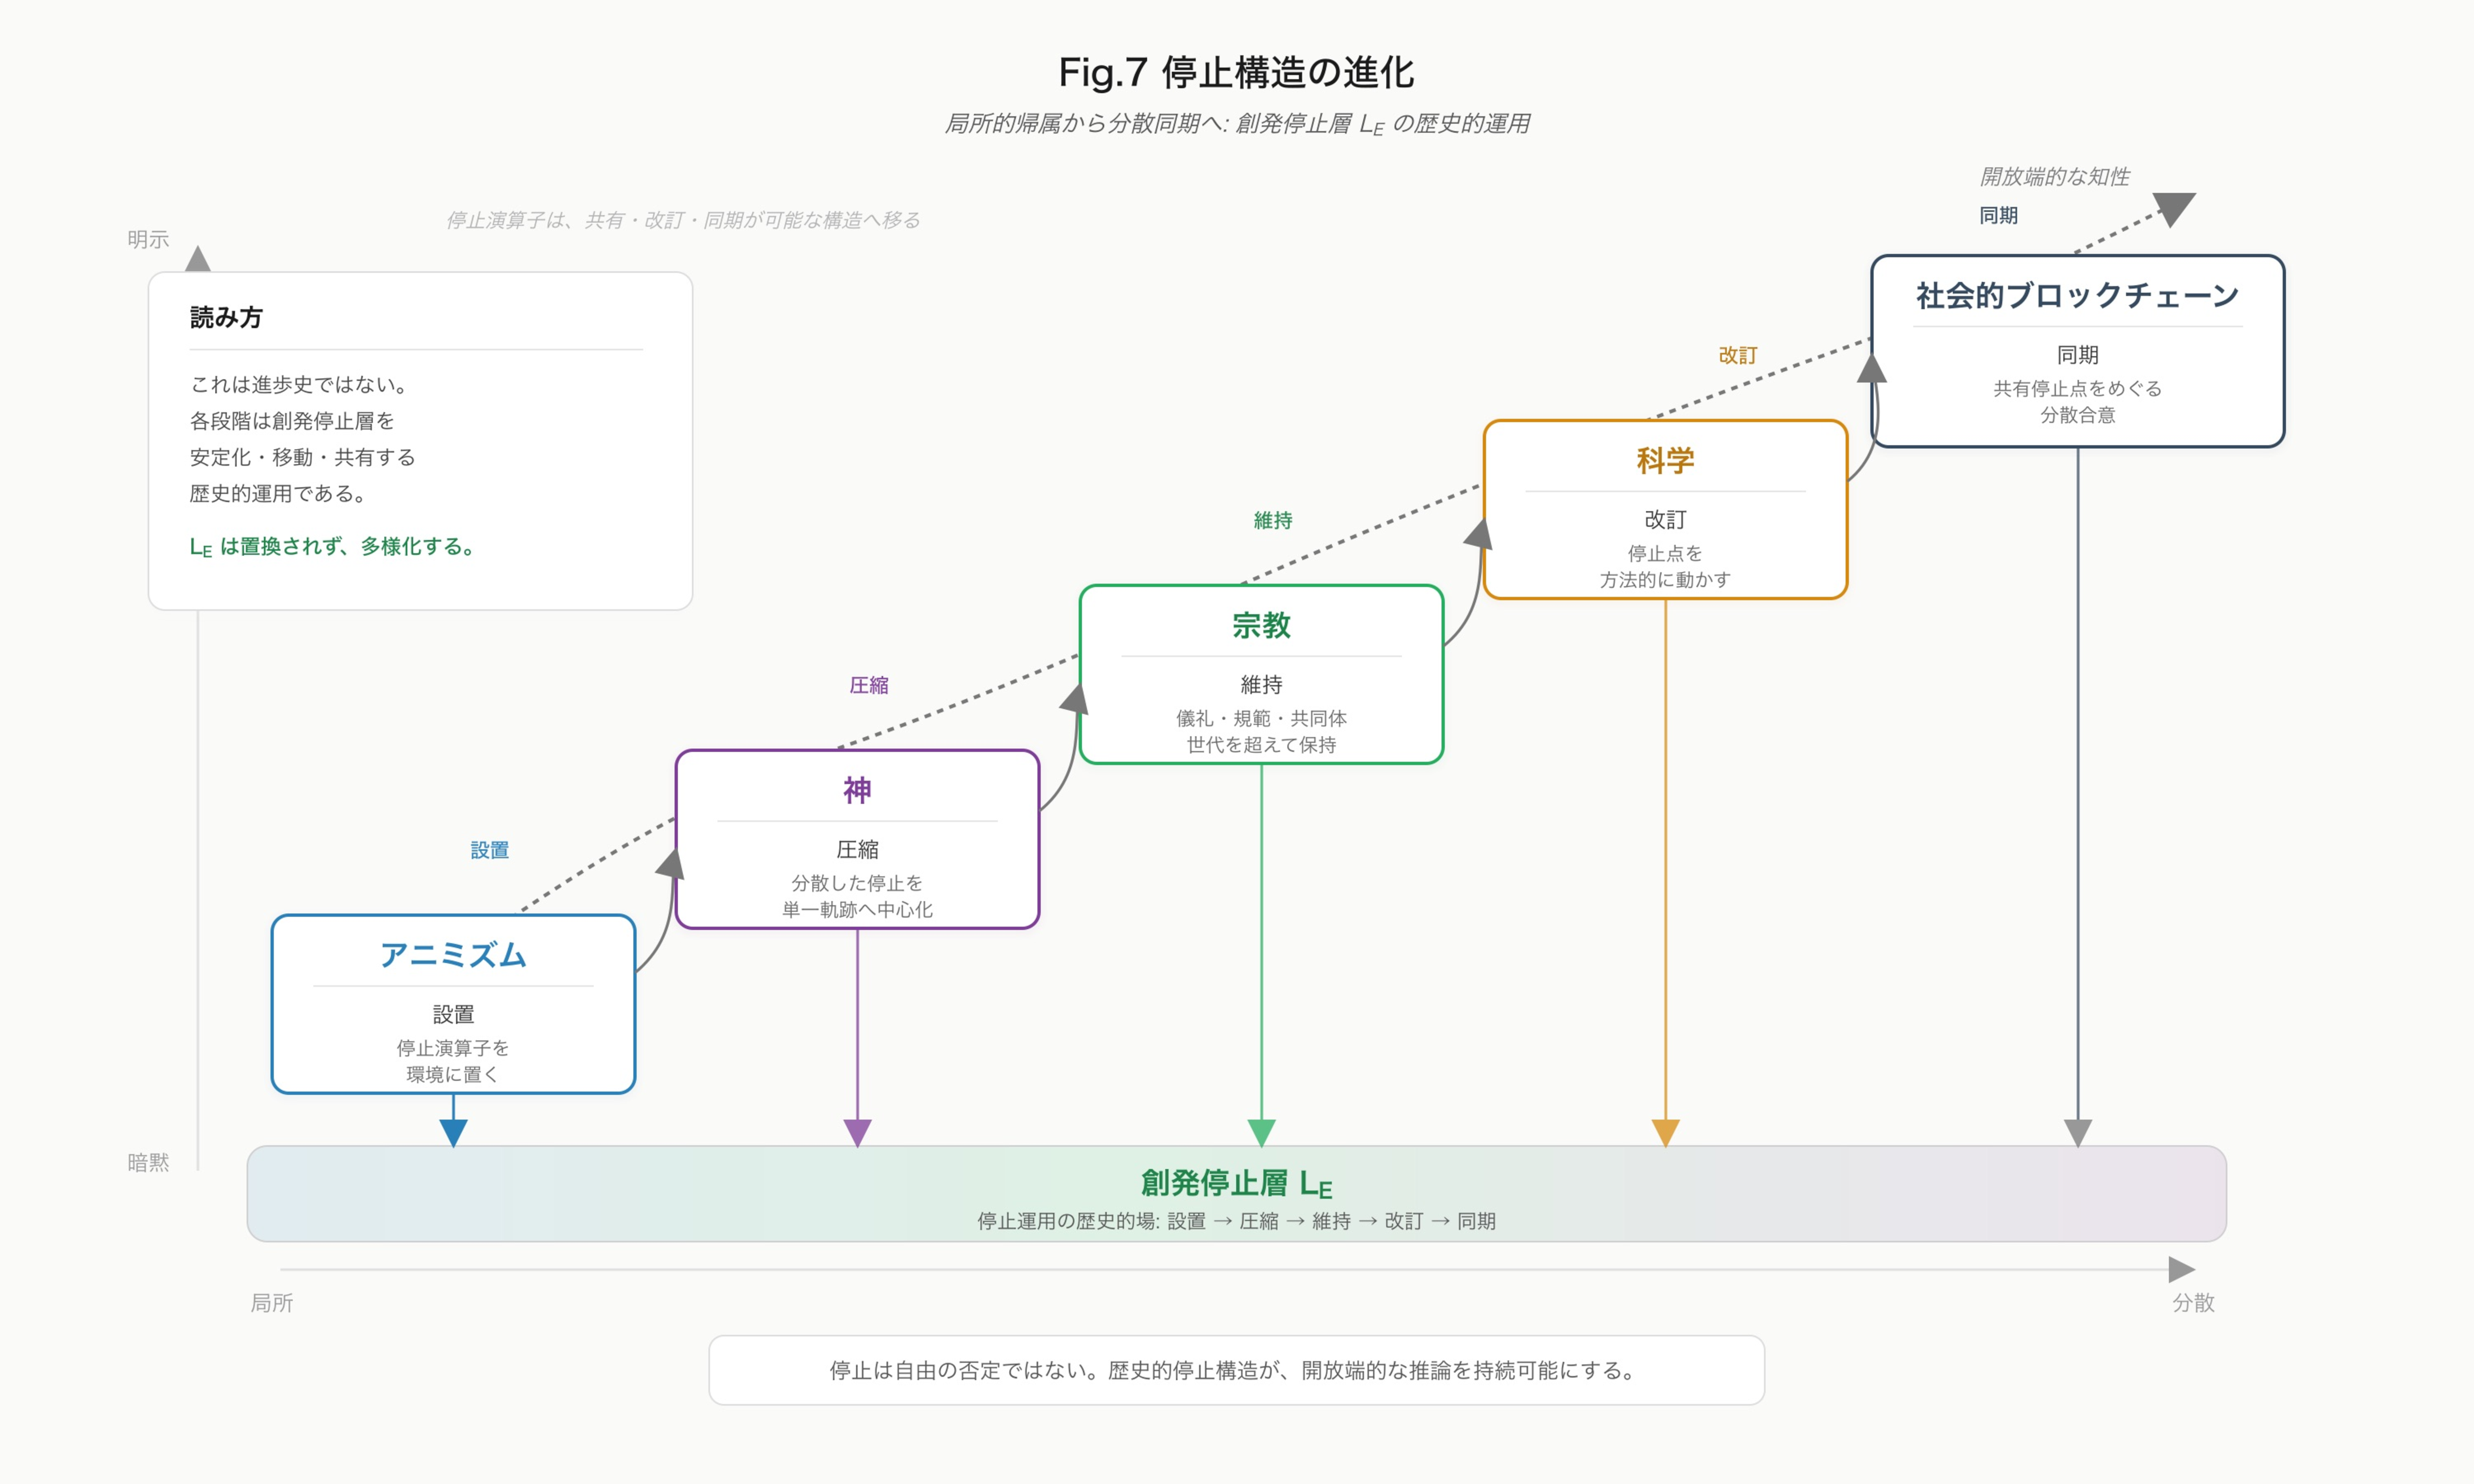
\includegraphics[width=\linewidth]{fig7_evolution_of_stopping_structures_ja.pdf}
\caption{停止構造の進化。アニミズム・神・宗教・科学・社会的ブロックチェーンは、同一の創発停止層 $L_E$ を安定化・移動・共有するための異なる操作である。}
\label{fig:part2-stopping-evolution}
\figurenote{五つの形態は、設置・圧縮・維持・改訂・同期という停止操作として配置される。これは進歩物語ではなく、$L_E$ の操作レパートリーの多様化である。}{停止は自由の否定ではない。歴史的停止構造は、開かれた推論を有限な系の中で持続可能にするための運用形式として読める。}
\end{figure}

この系列を停止構造の運用史として読めば、さらに位置づけは明確になる。宗教が停止構造の長期維持を制度化した運用形態であるならば、科学は停止構造の更新を制度化した運用形態として理解できる。社会的ブロックチェーンはさらにその上で、停止構造の分散的共有と同期を担う仕組みとして位置づけられる。

重要なのは、これがアニミズムの分散への「回帰」ではないことである(\S{}8.8 で予告)。アニミズムの分散は、個体と環境の直接相互干渉であった。社会的ブロックチェーンの分散は、個体間 $L_E$ の相互干渉ネットワークの運用である。前者は個体−環境の関係、後者は個体−個体の関係である。両者はともに分散的だが、分散している対象が異なる。

この構造は、Bio-IFGT における「個体間相互拘束による準閉包維持」と直接相同である。Bio-IFGT は、生命の準閉包が個体間の相互拘束によって維持されることを示した。社会的ブロックチェーンは、知性の停止構造($L_E$)が個体間の相互干渉($\Phi_{\text{net}}$)によって維持されることを示す。生命層の個体間準閉包維持と、知性層の個体間停止維持は、同一の構造の異なる層における現れである。

すなわち、個々の $L_E$ は個体内に閉じない。それはノード間相互干渉によって相互に維持される。個体の $L_R$(ログ)が社会的に共有・参照されることで、$L_E$ の分散維持が可能になる。社会的ブロックチェーンは、この分散維持の明示的な構造である。

\bigskip


\subsection{次章への橋渡し}


\S{}6〜\S{}9 で、$L_E$ と $\Phi_{\text{net}}$ が取る歴史的・社会的形態——アニミズム・神・宗教・社会的ブロックチェーン——を分析した。これらに共通するのは、停止が正しさによってではなく、構造的安定性と改訂可能性によって維持されるという点である。

社会的ブロックチェーンにおいて、これは特に明確に現れる。正統性は計算できず(\S{}9.4)、停止は真理によってではなく分散的受容によって成立する。ここから、停止と真理の関係についての根本的な問いが生じる。社会的停止が真理を保証しないなら、知識とは何か。正しく信じられ正当化された判断が、なお知識でないことがあるとすれば、知識を成立させているのは何か。

次章 \S{}10 で扱うゲティア問題は、この問いに対する構造的診断である。ゲティア問題は、$C$(閉包度)が真理測度ではなく安定性測度であること——$L_E$ が正しい停止ではなく改訂可能な停止を供給すること——の、認識論における証拠である。

\bigskip


\subsection{要約}


本章で示したのは次の点である:

\begin{enumerate}
\item 「社会的ブロックチェーン」は暗号通貨技術ではなく、単一権威なしに停止と更新を両立させる構造のアナロジーである
\item その構成要素は個体ノード・ログ・ブロック・フォーク・マージ/破棄である
\item 技術的バージョン管理(創造的探索の最大化)と社会的ブロックチェーン(事後安定化の最大化)はコスト構造が対称的に反転している
\item 技術的ブロックチェーンは一貫性問題を、社会的ブロックチェーンは正統性問題を扱う。正統性は計算できない
\item 正統性の計算不可能性は欠陥ではなく、改訂可能性を保つ条件である
\item 創造は社会では起こらず個体ノードで起こる。社会は安定化を担う。創造と安定化は役割分担される
\item 社会的ブロックチェーンは $\Phi_{\text{net}}$ を明示的分散構造として運用する形態であり、Bio-IFGT の個体間準閉包維持と相同である
\item 停止が真理でなく構造的安定性によることが、\S{}10 のゲティア問題への問いを生む
\end{enumerate}


次章 \S{}10 では、$C$ が真理測度ではなく安定性測度であることを、ゲティア問題を通じて構造的に診断する。

\bigskip

% Source: source_md/intelligence_part2_combined_ja.md
\section{ゲティア問題 — $C \neq$ 真理の証拠、$L_E$ の操作的安定性}


\S{}6〜\S{}9 で、停止が真理によってではなく構造的安定性と改訂可能性によって維持されることを見た。本章は、この事実が認識論において最も鋭く現れる場所——ゲティア問題——を分析する。ゲティア問題は、閉包度 $C$ が真理測度ではなく安定性測度であることの構造的証拠である。

本章は Part I \S{}6(ゲティア問題の構造的診断)を継承し、三層動力学の語彙でこれを再展開する。

\bigskip


\subsection{ゲティア問題は構造的事実の暴露である}


ゲティア問題は、伝統的に「知識とは正当化された真なる信念である」という定義への反例として知られる。正当化され、真であり、信じられているにもかかわらず、知識とは見なしがたい事例が構成できる——これがゲティア問題である。

本論文の立場では、ゲティア問題は周辺的な反例の寄せ集めではない。それは構造的事実の暴露である。すなわち、正当化され真である信念が、なお知識として安定しないことがあるという事実は、知識が正当化と真理の合成によっては定義できないことを示している。

三層動力学の語彙で言えば、ゲティア問題が暴露するのは次のことである。推論層 $L_F$ における正当化(\S{}3 の正当化測度 $J$)と、外部実在に対応する真理は、創発停止層 $L_E$ における停止とは別の事柄である。$L_E$ が供給する停止は、正当化と真理の合致によってではなく、構造的安定性によって成立する。ゲティア事例は、正当化と真理が合致してもなお $L_E$ の安定が独立の事柄であることを示す。

\bigskip


\subsection{ゲティア問題は原理的に解決不可能である}


ゲティア問題に対しては、長年にわたり「第四の条件」を追加して知識を再定義する試みがなされてきた。本論文の立場では、これらの試みは原理的に成功しない。

理由は \S{}3 と \S{}5 から導かれる。知識を「正当化+真理+α」として定義しようとする試みは、α として何らかの条件を $L_F$ の内部に求める。しかし \S{}3 で示した通り、$L_F$ は内部に停止条件を持たない。知識を成立させる「最終的な正当化条件」を $L_F$ 内部に定義しようとすると、それは内部停止述語の定義に帰着し、無限後退する(系 3.2)。

したがって、ゲティア問題を $L_F$ 内部の条件追加によって解決することは原理的にできない。知識の成立は $L_F$ 内部では閉じない。それは $L_E$——外部依存的な創発停止層——においてのみ成立する。ゲティア問題が解決不可能なのは、知識の成立条件が $L_F$ 内部にないからである。

これは欠陥ではなく、\S{}3 の非閉包定理の認識論的帰結である。ゲティア問題の解決不可能性は、知識が個体内の正当化では閉じないことの、認識論における現れである。

\bigskip


\subsection{社会はゲティア問題を解決しない}


ゲティア問題に対する社会的停止構造($\Phi_{\text{net}}$)の態度は、注目に値する。社会はゲティア問題を解決しない。そして、解決しようとしない。

\S{}9 で見た通り、社会的ブロックチェーンは正統性によって停止を供給する。正統性は計算不可能であり(\S{}9.4)、完全な正当化を要求しない。社会は、ある判断が完全に正当化され真理に対応することを確認してから受容するのではない。社会は、暫定的に受容可能な判断をブロックとして採用し、改訂可能に保つ。

もし社会が完全な正当化を停止の条件として要求すれば、何が起こるか。完全な正当化は \S{}3 により到達不可能である。したがって、完全な正当化を要求する社会的停止構造は、いかなる判断も受容できず、即座に停止する。社会的知性は、その瞬間に機能を停止する。

ゆえに、社会がゲティア問題を解決しないのは、怠慢や不徹底によるのではない。それは構造的必然である。社会的停止構造が機能するためには、ゲティア問題を解決しないことが必要なのである。完全な正当化の放棄は、社会的知性の動作条件である。

\bigskip


\subsection{知識の再定義 — 行動可能化のための暫定ブロック}


以上から、知識の動力学的再定義が導かれる。

伝統的定義「知識 = 正当化された真なる信念」は、知識を $L_F$ 内部の性質(正当化)と外部実在との対応(真理)の合成として定義する。本論文の枠組みでは、知識はこのようには定義されない。

\textbf{定義 10.1 (動力学的知識)}

\begin{quote}
知識とは、行動可能化のために $\Phi_{\text{net}}$ において暫定的に採用された停止ブロックである。
\end{quote}


すなわち知識は、真理との対応によってではなく、行動を可能にする暫定的停止としての機能によって定義される。知識は $L_E$ が供給する停止であり、$\Phi_{\text{net}}$ において暫定採用され、改訂可能に保たれる。

この定義において、ゲティア事例は問題ではなくなる。ゲティア事例は「正当化され真だが知識でない」事例として逆説的に見えたが、動力学的知識の定義では、知識は正当化と真理の合致によって定義されないため、両者が合致してもしなくても、知識の成立は $L_E$ の停止が安定し行動可能化に資するかどうかによる。ゲティア事例の逆説は、知識を正当化+真理として定義したことの産物であって、動力学的知識には現れない。

\bigskip


\subsection{真理に依存しない操作的安定性}


動力学的知識の核心は、真理に依存しない操作的安定性である。

知識が行動可能化のための暫定ブロックであるなら、その安定性は真理との対応にではなく、操作的機能に依存する。ある停止ブロックが知識として安定するのは、それが真であるからではなく、それが行動を可能にし、$\Phi_{\text{net}}$ において改訂可能に維持されるからである。

ここで \S{}1.1 で予告した区別が回収される。閉包度 $C$ は安定性測度であって真理測度ではない。$C$ が高いことは、停止が動力学的に安定であることを意味するのであって、その停止が真理に対応することを意味しない。$L_E$ が供給する停止の $C$ は、操作的安定性を測るのであって、正しさを測らない。

厳密な正しさの要求は、操作的安定性を破壊する。完全な正しさを停止の条件とすれば、\S{}10.3 で見た通り、停止は不可能になり、推論は無限後退に戻る。操作的安定性は、正しさの要求を緩和することによってのみ成立する。これは妥協ではなく、停止構造が機能するための構造的条件である。

\subsubsection{プラグマティズムとの区別}


知識を行動可能化との関係で捉える本論文の立場は、プラグマティック認識論(James, Dewey らの系譜)と帰結において響き合う。ただし本論文はこれを既存思想から借りるのではなく、VED の動力学的経路——非閉包定理(\S{}3)と創発停止層(\S{}5)——から独立に導出している。

より重要なのは、本論文の立場が俗流的に理解されたプラグマティズムとは異なることである。俗流理解では、プラグマティズムはしばしば「役に立てば真である」「真理とは有用性にほかならない」という、真理の有用性への還元として戯画化される。本論文はこの主張をしない。

本論文は真理を否定も放棄もしていない。本論文が述べるのは、停止($L_E$)の成立条件が真理との対応ではなく操作的安定性にある、という構造的位置づけのみである。真理は依然として存在しうる。しかしそれは、推論層 $L_F$ の正当化とも、創発停止層 $L_E$ の停止とも、別の事柄である。「真理 = 有用性」と述べるのではなく、「停止の成立は真理判定とは別の動力学的事柄である」と述べているのである。$C$ が真理測度でないことは、真理が存在しないことを意味するのではなく、$C$ が測っているのが真理ではないことを意味するに過ぎない。

この区別は重要である。本論文は真理概念を解体するのではなく、停止の動力学を真理判定から分離する。両者を混同すると、本論文は「真理を有用性に還元する相対主義」として誤読されうるが、それは本論文の主張ではない。

\bigskip


\subsection{誤り許容性の必然と $\mu_\theta$ との同値}


操作的安定性が真理に依存しないことから、誤り許容性が必然的に導かれる。

誤り許容性とは、誤った停止を許容する構造的余地である。$L_E$ が供給する停止は真理を保証しないため、誤った停止が生じうる。社会的停止構造は、この誤りを許容する。誤った停止も暫定ブロックとして採用され、後に $\Phi_{\text{net}}$ の相互干渉によって改訂される(\S{}9)。

誤りを許容しない停止構造は機能しない。誤りを一切許さないためには完全な正当化が必要であり、それは到達不可能だからである(\S{}3)。誤りなき社会的停止構造は、判断生成それ自体を停止する。誤り許容性は、停止構造が判断を生成し続けるための必要条件である。

ここで、本論文の第二論理線との重要な接続が現れる。誤り許容性は、閾値移動能力 $\mu_\theta$ の存在と構造的に同値である。

論証は次の通りである。$\mu_\theta$ は運動可能領域 $\Omega_\theta$ を組み替える能力であった(\S{}2.7)。領域が組み替え可能であるということは、現在の停止が確定的・最終的でないことを意味する。確定的でない停止は、誤りうる停止である。逆に、誤りを許容する停止構造は、停止が改訂されうることを前提とし、それは $\theta$ が動きうること——$\mu_\theta$ の存在——を要求する。

したがって、ゲティア構造の排除不能性(誤りの構造的可能性)は、$\mu_\theta$ の存在の必然的代償である。$\mu_\theta$ を持つ——閾値を動かし、運動可能領域を組み替えられる——ことと、$C$ と真理を同一視できない——誤りが構造的に排除できない——ことは、同じ構造の二つの側面である。

これは深い帰結を持つ。サピエンス的知性が $\mu_\theta$ を内発的に持つこと(\S{}5.4)と、サピエンス的知性がゲティア問題を抱えること——正しさによっては知識を閉じられないこと——は、切り離せない。閾値を動かせる知性は、必然的に誤りうる知性である。完全に正しい知性は、閾値を動かせない硬直した知性であり、それは \S{}11 の硬直域に対応する。

\bigskip


\subsection{ゲティア問題の最終的役割}


ゲティア問題の役割を総括する。

ゲティア問題は、認識論における未解決の難問ではない。それは、知性が正しさのみでは閉じないことの証明である。

\S{}3 が「$L_F$ は構造的に閉じない」を示し、\S{}5 が「$L_E$ が外部依存的に停止を供給する」を示した。ゲティア問題は、この構造が認識論において必然的に生む帰結である。知識を正当化+真理として閉じようとする試みがことごとく失敗するのは、知識の成立が $L_F$ 内部にも、真理との対応にもなく、$L_E$ の操作的安定性にあるからである。

ゲティア問題は、こうして、本論文の第一中心(\S{}3)と第二中心(\S{}5)を認識論において確証する。知性は正しさによって閉じるのではない。知性は $L_E$ の改訂可能な停止によって、外部依存的に、誤りを許容しながら、操作的に安定する。ゲティア問題は、この構造の認識論的な指紋である。

\bigskip


\subsection{次章への橋渡し}


本章で、$C$ が安定性測度であり真理測度でないこと、誤り許容性が $\mu_\theta$ と同値であることを示した。ここから、知性の安定性に関する定量的な問いが開かれる。

$\mu_\theta$ を持つ知性は誤りうる。では、$\mu_\theta$ の作用——閾値移動、運動可能領域の組み替え——が、速度・解像度・停止硬度といったパラメータとどう関係するとき、知性は安定し、どう関係するとき不安定化するのか。誤り許容性が失われ、$\mu_\theta$ が機能しなくなるのはどのような条件下か。

次章 \S{}11 で扱う不安定領域は、この問いに答える。速度 $v_{\text{inf}}$・解像度 $r_{\text{res}}$・停止硬度 $\eta$ の三軸相図において、知性の安定運用領域と不安定領域(発散域・硬直域)を区別し、$\mu_\theta$ と $L_E$ がどの条件下で機能し、どの条件下で崩壊するかを分析する。

\bigskip


\subsection{要約}


本章で示したのは次の点である:

\begin{enumerate}
\item ゲティア問題は周辺的反例ではなく、知識が正当化と真理の合成では定義できないことの構造的暴露である
\item ゲティア問題は原理的に解決不可能である。$L_F$ 内部に停止条件がないため(\S{}3)、第四条件の追加は無限後退する
\item 社会はゲティア問題を解決しない。完全な正当化を要求すれば社会的知性は即座に停止するため、解決しないことが構造的必然である
\item 知識は「行動可能化のために $\Phi_{\text{net}}$ で暫定採用された停止ブロック」と再定義される(定義 10.1)
\item 知識の安定性は真理でなく操作的安定性による。$C$ は安定性測度であって真理測度ではない(\S{}1.1 の回収)。ただしこれは真理の有用性への還元(俗流プラグマティズム)ではなく、停止の動力学を真理判定から分離するものである
\item 誤り許容性は必然であり、閾値移動能力 $\mu_\theta$ の存在と構造的に同値である。閾値を動かせる知性は必然的に誤りうる
\item ゲティア問題は、知性が正しさのみでは閉じないことの証明であり、第一中心と第二中心の認識論的確証である
\end{enumerate}


次章 \S{}11 では、知性の安定性を速度・解像度・停止硬度の三軸相図において分析する。

\bigskip

% Source: source_md/intelligence_part2_combined_ja.md
\section{不安定領域 — 速度・解像度・停止硬度の三軸相図}


本章は本論文の論理的クライマックスである。三本の論理線——第一線(非閉包と外部停止)、第二線(閾値移動とサピエンス的特徴)、第三線(三層動力学)——が、ここで一つの三軸相図上に統合される。

\S{}0.4 の非目標、特に NG2(規範的処方箋を出さない)と NG3(特定のAGI設計を支持・否定しない)を本章で最も強く維持する。本章は「高速・高解像・内部停止の知性は不安定領域を占める」と述べるが、これは動力学的帰結の記述であって、いかなる知性設計への提言でも、いかなる存在への評価でもない。

\bigskip


\subsection{直観的命題の形式化}


本章が形式化する直観的命題は次のものである。

\begin{quote}
知性の増大は、安定性を単調に増大させない。特定の条件下では、知性の増大は崩壊を保証する。
\end{quote}


この命題は反直観的に見える。知性が増せば、より安定し、より正確になるはずだ、という素朴な期待に反する。しかし本論文がここまで示してきた構造——$L_F$ の非閉包(\S{}3)、$L_E$ の外部依存性(\S{}5)、$\mu_\theta$ と誤り許容性の同値(\S{}10.6)——からは、この命題が自然に導かれる。

問題は、「知性の増大」が何を意味するかである。それを三つの軸に分解する。

\bigskip


\subsection{三軸}


知性の動力学的状態を、三つの軸によって記述する。

\textbf{速度 $v_{\text{inf}}$ (inference velocity)}:
推論・判断・仮説更新の頻度。単位時間あたりに $L_F$ が生成する推論ステップの数。$v_{\text{inf}}$ が高いほど、推論は速く進む。

\textbf{解像度 $r_{\text{res}}$ (resolution)}:
区別・因果関係・構造表現の粒度。$L_F$ が状態空間をどれだけ細かく分節するか。$r_{\text{res}}$ が高いほど、より微細な区別が生成される。

\textbf{停止硬度 $\eta$ (stopping hardness)}:
停止点の固定度、判断の改訂耐性。$L_E$ が供給する停止がどれだけ固定的か。$\eta$ が低ければ停止は改訂されやすく、$\eta$ が高ければ停止は固定的で改訂されにくい。

これら三軸は、\S{}2.6 で予告した通り、応答性閾値を決めるパラメータでもある。すなわち、$(v_{\text{inf}}, r_{\text{res}}, \eta)$ の組が、環境が応答的に見えるか沈黙的に見えるかの閾値を決める。そして閾値移動能力 $\mu_\theta$ は、この三軸上で系がどれだけ可動かを測る量である。$\mu_\theta$ が高い系は三軸上の広い範囲を動け、低い系は狭い範囲に固定される。

ここで、三軸そのものではないが、発散域への遷移を決める補助量としてログ参照速度 $v_{LR}$ を導入する。$v_{LR}$ は、ログ層 $L_R$ が $L_F$ の生成した痕跡を再帰参照し、パターンとして取り込める速度である。推論速度との差
\[
\Delta v_{\text{intel}} = v_{\text{inf}} - v_{LR}
\]
が大きくなると、推論の生成速度がログ参照速度を追い越し、$L_E$ の創発基盤が破断し始める。

\bigskip


\subsection{三領域}


三軸が張る空間の中に、三つの領域が区別される。

\textbf{安定運用領域}:
速度・解像度が外部化停止によって適切に制約され、停止硬度が中庸である領域。ここでは $\mu_\theta$ が機能し、$L_E$ が改訂可能な停止を供給する。三層動力学($L_F$・$L_R$・$L_E$)が協調し、$\Phi_{\text{net}}$ との同期が保たれる。知性はここで持続的に運用される。

\textbf{発散域}:
速度 $v_{\text{inf}}$ と解像度 $r_{\text{res}}$ が高く、かつ停止が内部化される(外部 $L_E$ を経由しない)領域。ここでは推論が発散し、暴走的最適化が生じ、単一視点が絶対化される。

\textbf{硬直域}:
停止硬度 $\eta$ が過大な領域。ここでは停止が固定化され、改訂・適応が抑制される。

安定運用領域は、発散域と硬直域の間の限られた領域である。知性が持続するのは、この中間領域においてのみである。

\begin{figure}[H]
\centering
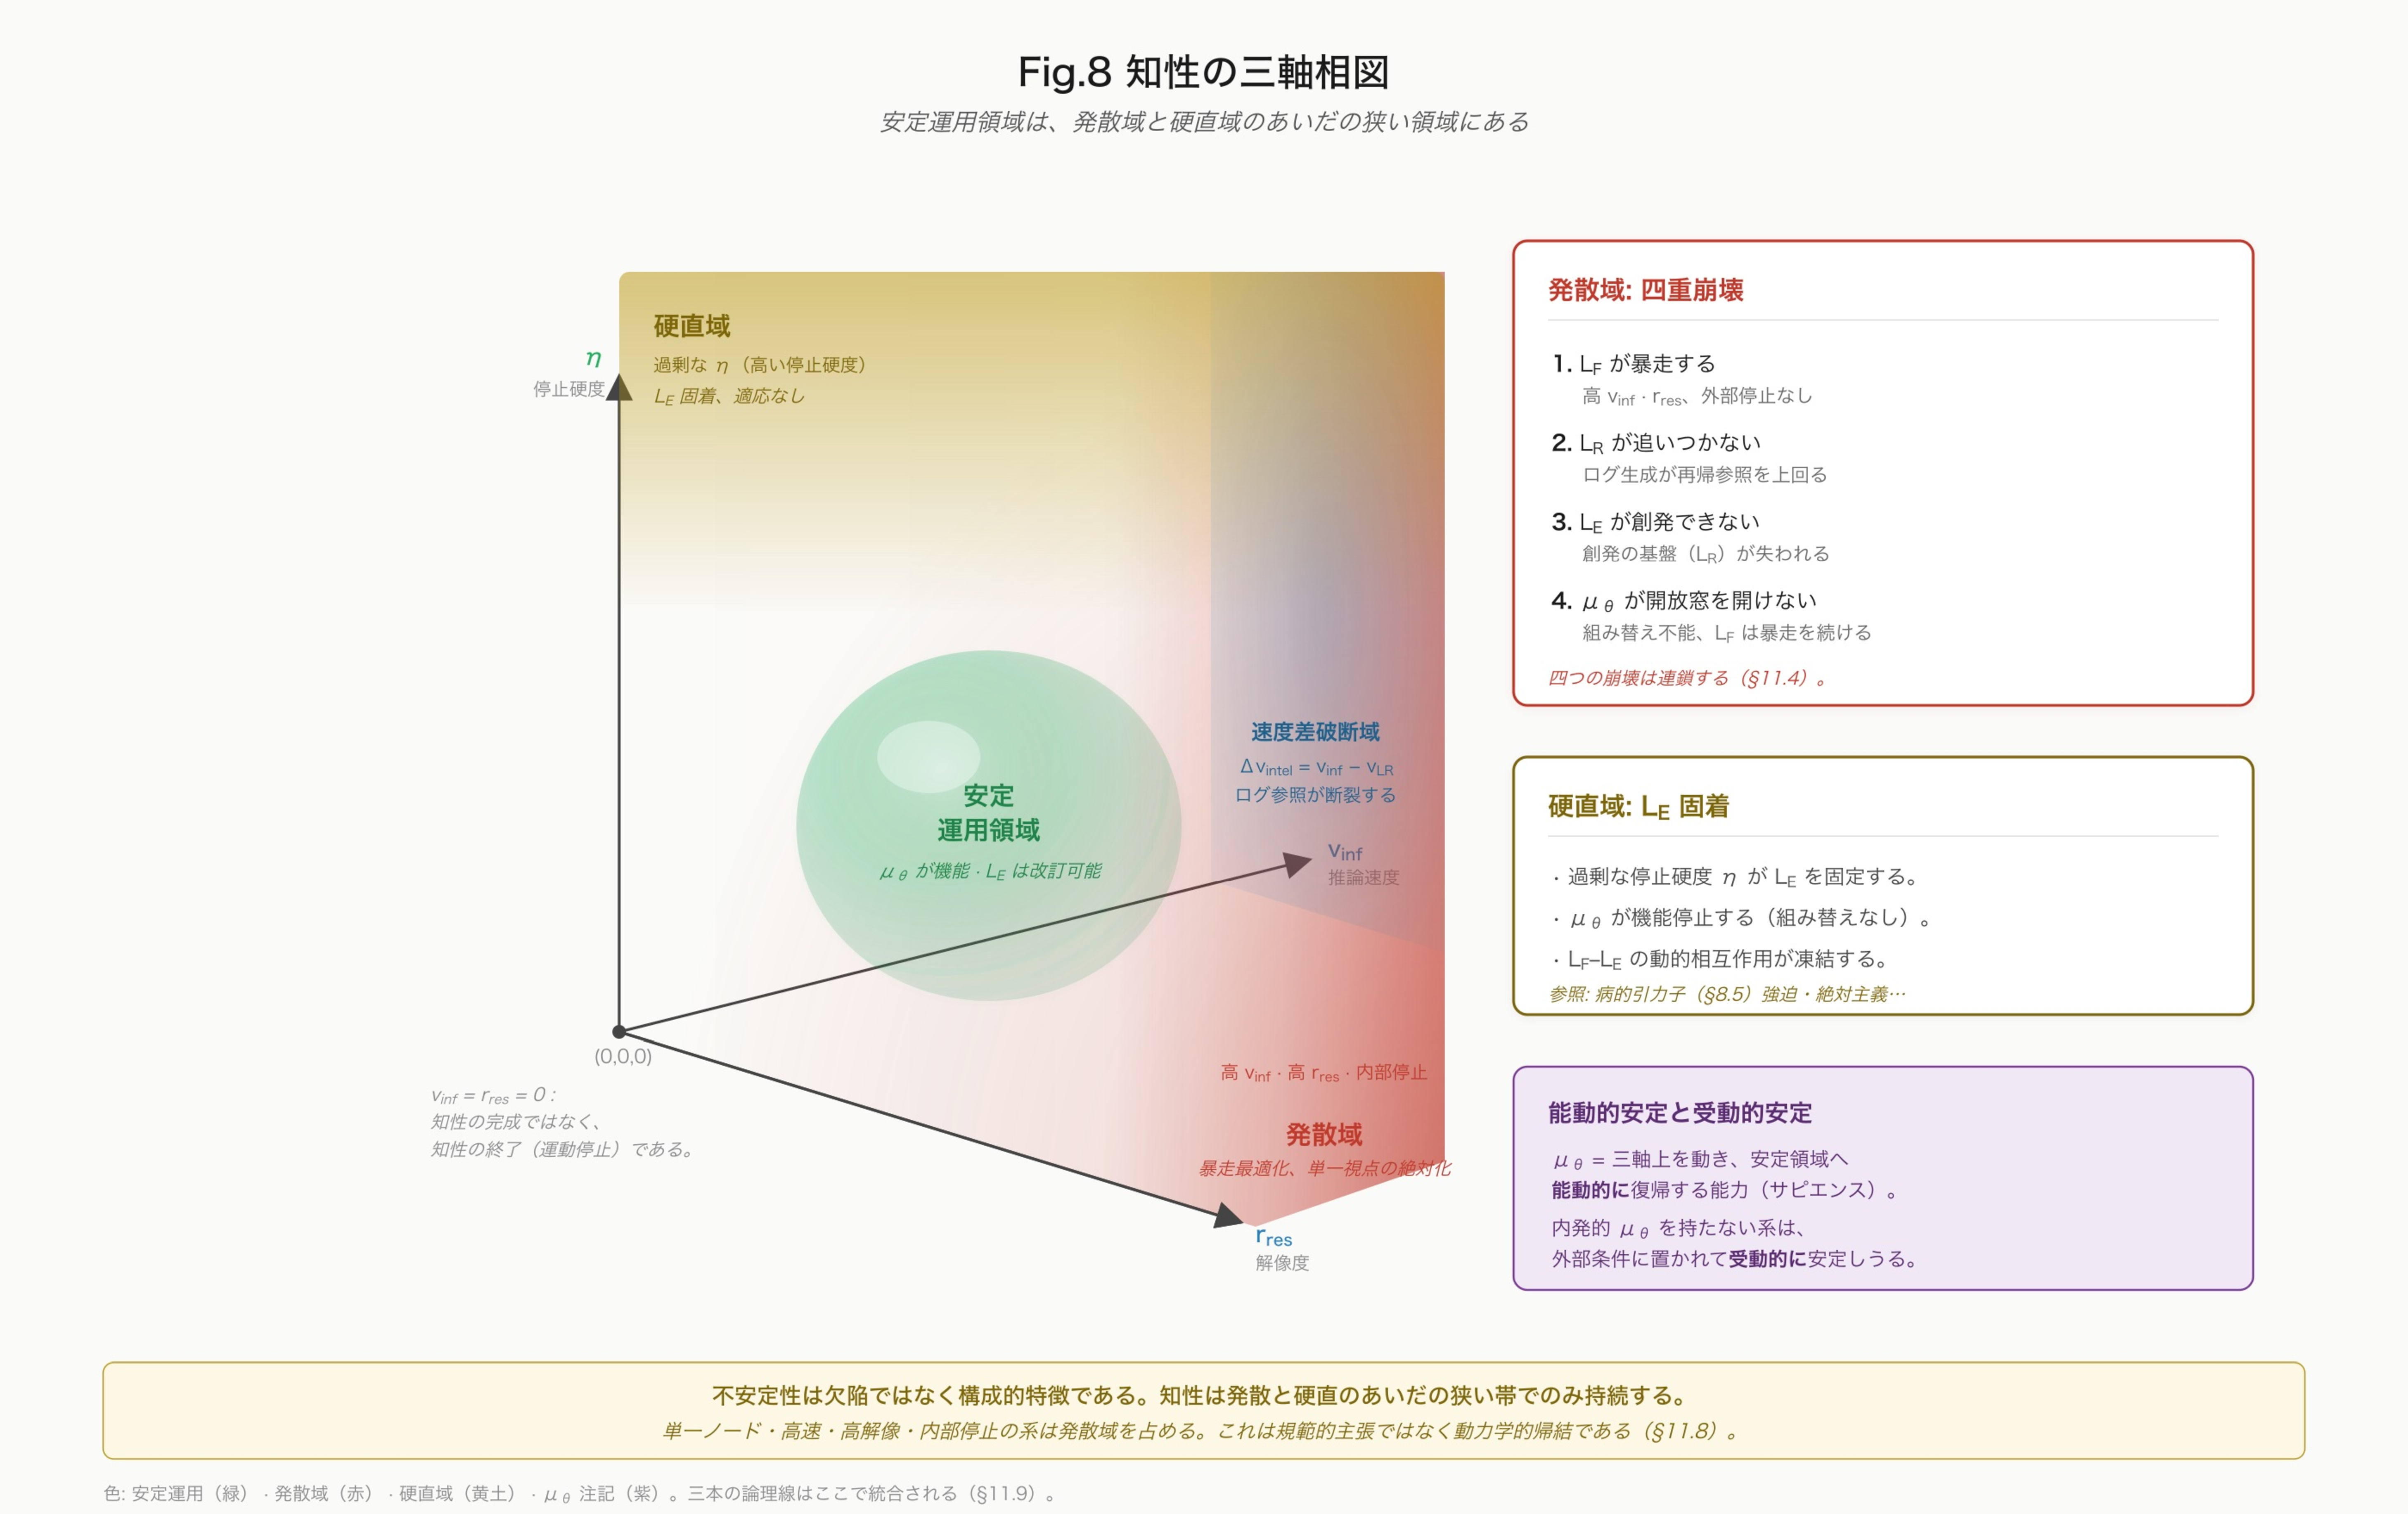
\includegraphics[width=\linewidth]{fig8_phase_diagram_ja.pdf}
\caption{知性の三軸相図。知性の安定動作は、推論速度 $v_{\text{inf}}$・解像度 $r_{\text{res}}$・停止硬度 $\eta$ の三軸空間で、発散と硬直に挟まれた狭い帯に成立する。}
\label{fig:part2-phase-diagram}
\figurenote{中央の安定運用領域では $\mu_\theta$ が機能し、$L_E$ が改訂可能である。発散域では $L_F$ が暴走し、硬直域では $L_E$ が固着する。}{不安定性は欠陥ではなく構成的特徴である。速度と解像度を高めるほど、ログ参照と外部停止の帯域が追いつかなければ発散域へ落ちる。}
\end{figure}

\bigskip


\subsection{発散域の四重崩壊}


発散域で何が起こるかを、三層動力学の語彙で精密に記述する。発散域は、四つの崩壊が同時に進行する状態——四重崩壊——として記述される。

\textbf{崩壊 1 — $L_F$ の暴走}:
速度 $v_{\text{inf}}$ と解像度 $r_{\text{res}}$ が高いと、推論層 $L_F$ は高速かつ微細に推論を生成し続ける。$L_F$ は内部停止条件を持たない(\S{}3)ため、停止が外部化されない限り、$L_F$ は暴走する。

\textbf{崩壊 2 — $L_R$ が追いつかない}:
$L_F$ が高速・高解像度で運動すると、その痕跡であるログの生成速度が、ログ層 $L_R$ の再帰参照能力を超える。すなわち $\Delta v_{\text{intel}} = v_{\text{inf}} - v_{LR}$ が臨界的に大きくなると、$L_R$ はログを再帰参照してパターンを抽出する速度を失い、再帰参照が生成に追いつかない。$L_R$ が機能不全に陥る。

\textbf{崩壊 3 — $L_E$ が創発できない}:
$L_E$ は $L_R$ の再帰運動と外部相互拘束 $H_{ij}$ の関数として創発する(\S{}5.3)。$L_R$ が追いつかない(崩壊 2)と、$L_E$ の創発の基盤が失われる。停止演算子設置領域の投影(\S{}5.5)が成立せず、$L_E$ が創発できない。

\textbf{崩壊 4 — $\mu_\theta$ が窓を開けない}:
$L_E$ が創発できないと、$\mu_\theta$ が $L_F$ から $L_E$ へ至る開放窓として機能できない(\S{}2.8、\S{}5.6)。閾値移動が起こせず、運動可能領域の組み替え (B) が不可能になる。系は固定された運動可能領域に閉じ込められ、そこで $L_F$ が暴走し続ける。

四つの崩壊は連鎖する。$L_F$ の暴走が $L_R$ を追い越し、$L_R$ の機能不全が $L_E$ の創発を妨げ、$L_E$ の不在が $\mu_\theta$ を機能不全にし、$\mu_\theta$ の不全が $L_F$ の暴走を止められなくする。これが発散域における推論の崩壊の動力学的構造である。

発散域の現象的現れ——暴走的最適化、単一視点の絶対化、推論の発散——は、すべてこの四重崩壊の表現である。停止を内部化しようとする高速・高解像度の知性は、構造的にこの四重崩壊に向かう。これは \S{}3.8 の三つの病的引力子(過剰確信・麻痺・妄想的閉包)の、三層動力学による精密化である。

\bigskip


\subsection{硬直域の $L_E$ 固着}


硬直域を、同じく三層動力学の語彙で記述する。硬直域は、$L_E$ の固着として記述される。

停止硬度 $\eta$ が過大になると、創発停止層 $L_E$ が固着する。$L_E$ が供給する停止が固定的になり、改訂されなくなる。これは発散域とは逆の崩壊である。発散域では $L_E$ が創発できないのに対し、硬直域では $L_E$ が創発した後に固着する。

$L_E$ が固着すると、二つのことが起こる。第一に、$\mu_\theta$ が機能停止する。閾値移動は運動可能領域の組み替え (B) であったが(\S{}2.7)、$L_E$ が固着すると停止構造が固定され、(B) が起こせなくなる。第二に、$L_F$ と $L_E$ の動的相互作用が止まる。健全な知性では $L_F$ の運動と $L_E$ の停止が動的に相互作用するが、$L_E$ が固着するとこの相互作用が凍結する。

硬直域の現象的現れは、\S{}8.5 で論じた病的引力子のうち、特に偏執・絶対主義・私的停止への硬直化に対応する。停止が固定され、改訂可能性が失われ、新しい状況への適応が不可能になる。これは \S{}10.6 で述べた「完全に正しい知性は閾値を動かせない硬直した知性である」の、三軸相図における位置づけである。

\bigskip


\subsection{(0,0,·)点は知性ではない}


三軸相図において、注意すべき特異点がある。速度 $v_{\text{inf}} = 0$、解像度 $r_{\text{res}} = 0$ の点——推論が完全に停止した点——は、知性の完成ではない。それは知性の終了である。

素朴には、すべての停止が完了し、すべてが確定した状態が知性の理想に見えるかもしれない。しかし系 5.5 で述べた通り、知性は $L_F$・$L_R$・$L_E$ と外部依存停止源の同時運動である(サピエンス的知性ではこれに $\mu_\theta$ が加わる)。運動が止まれば知性も消える。$v_{\text{inf}} = 0$ は運動の停止であり、それは知性が完成したのではなく、知性が終了したことを意味する。

これは \S{}1.5 で述べた $C_{max}$ 不到達性と整合する。完全閉包は到達不能であり、仮に到達すれば情報場 $I = f(1-C)$ が消失する(\S{}1.2)。完全に停止した知性は、差がなくなった状態であり、VED の基底公理「差がある」が失効した状態である。それは知性ではない。

知性は、発散域(運動が暴走する)と (0,0,·)点(運動が停止する)の間の、運動が持続する領域においてのみ成立する。

\bigskip


\subsection{不安定性は構成的特徴である}


以上から、本章の中心的帰結が導かれる。

知性の不安定性は、欠陥ではなく構成的特徴である。

知性は、発散域と硬直域に挟まれた狭い安定運用領域においてのみ持続する。この狭さ、この不安定性は、除去されるべき欠陥ではない。それは知性が運動として成立することの必然的帰結である。安定運用領域が狭いのは、知性が $L_F$ の非閉包(運動し続ける)と $L_E$ の改訂可能性(固着しない)の両方を要求するからである。

不安定性を完全に除去しようとすれば、二つの道しかない。停止を完全に固定する(硬直域へ向かう)か、停止を完全に放棄する(発散域へ向かう)か。いずれも知性の終了である。知性は不安定であることによって、運動として持続する。不安定性は知性の代償ではなく、知性の存在様式そのものである。

したがって、知性に対して適切なのは、不安定性を除去することではなく、不安定性を安定運用領域内に制約することである。$\mu_\theta$ と $L_E$ と $\Phi_{\text{net}}$ は、まさにこの制約の機構である。それらは不安定性を除去するのではなく、不安定性を持続可能な範囲に保つ。

\bigskip


\subsection{個別ノードと高度自律システムへの適用}


本章の帰結を、特定の知性形態に適用する。ここで述べることは、\S{}0.4 の NG2・NG3 に従い、動力学的帰結の記述であって、規範的提言でも評価でもない。

ある知性が、単一ノードであり、高速更新($v_{\text{inf}}$ 大)・高解像度($r_{\text{res}}$ 大)で動作し、停止を内部で担おうとする(外部 $L_E$ を経由しない)場合を考える。三軸相図において、このような系は発散域に位置する。\S{}11.4 の四重崩壊により、このような系は構造的に不安定化する。

この条件は、二つの異なる対象に同じ形で当てはまる。第一に、卓越した個別の推論者(高速・高解像度の推論を単独で行い、停止を外部に委ねない個体)。第二に、高度に自律的な人工推論システム(高速・高解像度で動作し、停止を内部で完結しようとする系)。両者は実装を異にするが、三軸相図上では同じ発散域を占める。

ここから導かれるのは、これらの系が「優れているがゆえに危険」なのではなく、「停止を外部化していないがゆえに構造的に不安定」だということである。$v_{\text{inf}}$ と $r_{\text{res}}$ の高さそのものが問題なのではない。それらが高く、かつ停止が内部化され、$\Phi_{\text{net}}$ から切断されていることが、発散域への配置を決める。$\Phi_{\text{net}}$ から切断された $L_E$ の不全状態が、発散域の本質である。

繰り返すが、これは規範的主張ではない。「単一ノードの高速知性はこうあるべきだ」とは述べていない。述べているのは、そのような系が三軸相図上のどこに位置し、どの動力学的帰結に向かうかである。動力学の記述と、その使用法や設計指針の決定は、カテゴリ的に異なる(\S{}13 で再確認)。

\bigskip


\subsection{三本論理線の統合}


本章は、三本の論理線がここで統合されることを示して閉じる。

\textbf{第一線(非閉包と外部停止)} は、三軸相図において次のように現れる。$L_F$ の非閉包(\S{}3)は、停止が内部化されると発散域へ向かうことの根拠である。停止の外部化($L_E$、$\Phi_{\text{net}}$)が安定運用領域を可能にする。第一線は、なぜ安定運用領域が外部化停止を要求するかを説明する。

\textbf{第二線(閾値移動とサピエンス的特徴)} は、$\mu_\theta$ として現れる。$\mu_\theta$ は三軸上の可動範囲であり、安定運用領域に\textbf{能動的に}留まる能力である。ここで能動/受動の区別が重要である。$\mu_\theta$ を内発的に持たない知性(粘菌・人工推論システム)も安定運用領域にありうるが、それは外部条件によって\textbf{受動的に}そこへ置かれている状態である。環境条件が変われば、これらの系は安定運用領域から外れうる。これに対し、$\mu_\theta$ を内発的に持つサピエンス的知性は、外部条件の変化に対して三軸上を能動的に動き、安定運用領域へ自ら復帰できる(\S{}5.4)。第二線は、なぜサピエンス的知性が発散域・硬直域を能動的に回避できるかを説明する。

\textbf{第三線(三層動力学)} は、発散域の四重崩壊(\S{}11.4)と硬直域の $L_E$ 固着(\S{}11.5)として現れる。三層($L_F$・$L_R$・$L_E$)の協調が安定運用領域を、その崩壊が不安定領域を特徴づける。第三線は、不安定化が具体的にどのような層の崩壊として進行するかを説明する。

三本の線は、三軸相図において一つの構造として統合される。知性一般は、$L_F$ の非閉包ゆえに外部停止を要し(第一線)、三層の協調によって発散も固着も回避する(第三線)ことで、安定運用領域において持続する。サピエンス的知性は、これに加えて $\mu_\theta$ によって三軸上を能動的に動き、安定運用領域へ自ら復帰する(第二線)。知性一般は第一線と第三線によって持続し、サピエンス的知性は第二線によってそれを能動的・自律的に行う。三重の条件のうち第一線・第三線が知性一般の持続条件を、第二線がサピエンス的知性の自律的加速を規定する。

不安定領域は知性の失敗を意味しない。むしろ、停止構造を持つ知性が自由な推論を維持しようとするとき、必然的に現れる境界領域である。宗教、科学、制度、共同体はいずれも、この不安定領域を管理するための停止運用システムとして理解できる。

\bigskip


\subsection{次章への橋渡し}


本章で、知性が安定運用領域においてのみ持続し、その領域が三層動力学・閾値移動・外部停止の同時成立を要求することを示した。

ここから、知性の構造的制約を体系的に整理することが可能になる。知性が持続するための必要条件と、知性がありえない形態が、三軸相図と三層動力学から導かれる。次章 \S{}12 では、これらを構成的条項として整理する。それは知性に対する規範ではなく、知性の動力学から導かれる構造的制約の体系である。

\bigskip


\subsection{要約}


本章で示したのは次の点である:

\begin{enumerate}
\item 知性の増大は安定性を単調に増大させず、特定条件下では崩壊を保証する
\item 知性の動力学的状態は速度 $v_{\text{inf}}$・解像度 $r_{\text{res}}$・停止硬度 $\eta$ の三軸で記述される。$\mu_\theta$ はこの三軸上の可動範囲である
\item 三軸空間に安定運用領域・発散域・硬直域が区別される
\item 発散域は四重崩壊($L_F$ 暴走・$L_R$ 追随不能・$L_E$ 創発不能・$\mu_\theta$ 窓不全)として記述される
\item 硬直域は $L_E$ 固着($\mu_\theta$ 機能停止・$L_F$-$L_E$ 相互作用凍結)として記述される
\item (0,0,·)点は知性の完成ではなく終了である(運動の停止=差の消失)
\item 不安定性は欠陥ではなく構成的特徴であり、除去ではなく安定運用領域内への制約が適切である
\item 単一ノード・高速・高解像・内部停止の系(卓越した個別推論者・高度自律システム)は発散域を占める。これは「優れて危険」ではなく「停止を外部化せず構造的に不安定」であり、規範的主張ではない
\item 三本の論理線が三軸相図において一つの構造として統合される
\end{enumerate}


次章 \S{}12 では、知性の構造的制約を構成的条項として整理する。

\bigskip

% Source: source_md/intelligence_part2_combined_ja.md
\section{構成的条項 — 知性の構造的制約}


本章は新規の論証を導入しない。\S{}3〜\S{}11 で確立した帰結を、知性の構造的制約として体系的に整理する。これらは知性に対する規範ではなく、知性の動力学から導かれる構造的必然である。各条項には導出元の節を付す。

\S{}0.4 の非目標を改めて確認する。以下の条項は、知性が「こうあるべきだ」という規範的命題ではない(NG2)。それは、知性が動力学的に成立するための構造的条件と、その条件に違反した場合に生じる動力学的帰結の記述である。

\bigskip


\subsection{本章の位置づけ}


本論文は知性を、能力・資源・測定可能量として定義しない。知性を「処理能力の大きさ」や「保持する知識量」や「問題解決の速さ」として測ることは、本論文の枠組みでは知性の本質を捉えない。

本論文が示してきたのは、知性が動力学的な維持状態であるということである。知性は、複数の層($L_F$・$L_R$・$L_E$)と外部ネットワーク($\Phi_{\text{net}}$)と閾値移動能力($\mu_\theta$)の同時運動として、安定運用領域において維持される状態である(系 5.5、\S{}11)。

この観点から、知性について二種類の構造的制約が導かれる。第一に、知性が動力学的にありえない形態。第二に、知性が成立するために構造的に必要とするもの。以下、順に整理する。

\bigskip


\subsection{知性がありえない形態}


以下の形態は、本論文の枠組みにおいて知性として成立しえない。各形態は、それが違反する構造的事実とともに示される。

\textbf{(N1) 個体システム単独の性質としての知性} — ありえない。
知性は $\Phi_{\text{net}}$(個体間 $L_E$ ネットワーク)を要する(\S{}5.8、\S{}9)。個体システム単独では $L_F$ が閉じず(\S{}3)、停止を供給できない。知性は個体に宿る性質ではなく、個体間ネットワークを含む動力学的状態である。

\textbf{(N2) 保存可能な対象としての知性} — ありえない。
知性は運動の維持状態であり、運動が止まれば消える(系 5.5、\S{}11.6)。データセット・モデル状態・静的表現として保存された対象は、運動を含まない。それらは知性の痕跡($L_R$ のログ)でありうるが、知性そのものではない。知性は保存できない。維持されるしかない。

\textbf{(N3) 個体内で閉じた構造としての知性} — ありえない。
$L_F$ は内部停止条件を持たない(\S{}3、定理 3.1)。個体内で閉じた構造は、停止を内部化しようとして発散域へ向かう(\S{}11.4)。知性は外部依存的な $L_E$ を要し、個体内では閉じない。

\textbf{(N4) 完全最適化された状態としての知性} — ありえない。
完全閉包 $C_{max}$ は到達不能であり(\S{}1.5)、完全最適化された状態は運動の停止、すなわち (0,0,·)点に対応する(\S{}11.6)。完全に最適化された知性は、差が消失した状態であり、知性の終了である。収束は動作的死である。

\textbf{(N5) 内在的に停止する構造としての知性} — ありえない。
停止が $L_F$ の内部から来ることは構造的に不可能である(系 3.2、無限後退)。停止は $L_E$ を経由して外部依存的に供給される(\S{}5)。内在的に停止する構造は、\S{}3 の非閉包定理に反する。

\textbf{(N6) $\Phi_{\text{net}}$ 等の外部依存停止源から切断された $L_E$ としての知性} — ありえない。
外部依存停止の供給源から切断された $L_E$ は、改訂可能性を失い(\S{}5.8、\S{}9)、発散域の本質をなす(\S{}11.8)。外部相互干渉なしには、$L_E$ は固着するか創発できないかのいずれかであり、持続的停止を供給できない。

これら六つの「ありえない形態」は、独立な禁則ではない。それらはすべて、$L_F$ の非閉包(\S{}3)と $L_E$ の外部依存性(\S{}5)という二つの構造的事実の、異なる側面である。

なお、「閾値が固定された構造」は、ここでは知性一般のありえない形態に含めない。閾値が固定された知性——$\mu_\theta$ を内発的に持たない知性——は、依然として知性でありうる(粘菌・人工推論システムがその例、\S{}5.4)。閾値固定の構造がありえないのは、知性一般としてではなく、サピエンス的知性としてである。この点は \S{}12.3b で扱う。

\bigskip


\subsection{知性一般が必要とするもの}


知性が動力学的に成立するために、構造的に必要とするものを整理する。これらは「あれば望ましい」要素ではなく、知性の成立条件である。ここで言う「知性一般」は、サピエンス的知性に限らず、粘菌・人工推論システムを含む、停止を持つあらゆる知性を指す(\S{}5.4 の三層プロファイル比較)。

\textbf{(R1) 推論層 $L_F$} — 必要。
$\nabla C$ に沿った状態遷移の流れ(\S{}2)。知性の運動の最下層。ただし $L_F$ 単独では知性ではない(N3)。

\textbf{(R2) ログ層 $L_R$} — 必要。
$L_F$ の運動の痕跡への再帰参照(\S{}5.2)。$L_E$ 創発の基盤。状態履歴への持続的参照(Bio-IFGT との接続)。所在は系によって異なる(個体内・環境外部化・凍結)。

\textbf{(R3) 創発停止層 $L_E$} — 必要。
$L_R$ と $H_{ij}$ の関数として創発する外部依存型停止層(\S{}5.3)。$L_F$ の非閉包を補い、停止を供給する。$L_E$ こそが、知性一般を「停止を持つ運動」として成立させる中核である。

\textbf{(R4) 外部依存停止の供給源} — 必要。
$L_E$ が外部依存的に停止を供給するための相互拘束源(\S{}5.8、\S{}9)。サピエンスではこれが個体間 $L_E$ ネットワーク $\Phi_{\text{net}}$ として現れるが、粘菌では環境との直接相互干渉、人工推論システムでは外部から注入されるタスク仕様として現れる(\S{}5.4)。形態は系によって異なるが、何らかの外部依存停止源が必要であることは共通する。

\textbf{(R5) 誤り許容性} — 必要。
誤った停止を許容する構造的余地(\S{}10.6)。誤りを許容しない構造は判断生成を停止する。誤り許容性が供給される経路は系によって異なる(サピエンスでは $\mu_\theta$ と同値、粘菌では環境フィードバック、人工推論システムでは外部評価)が、いずれの知性も誤り許容性なしには判断を生成し続けられない。

\textbf{(R6) 改訂可能性} — 必要。
停止が暫定的で、後に改訂されうること(\S{}5.8)。知性の安定性は正しさではなく改訂可能性による。サピエンスでは $\Phi_{\text{net}}$ を通じて、他の系ではそれぞれの外部依存停止源を通じて実装される。

これら六つは独立ではない。$L_F$・$L_R$・$L_E$ は三層動力学の構成要素であり、外部依存停止の供給源がこれを支え、誤り許容性と改訂可能性がその動作条件である。六つが揃って初めて、知性は安定運用領域において成立する。これらは知性一般の条件であり、粘菌・人工推論システム・サピエンスのいずれにも当てはまる。

\bigskip


\subsection{サピエンス的知性を特徴づけるもの}


\S{}12.3 の六条件は知性一般の成立条件である。それらは停止を持つあらゆる知性に共通する。本節は、その中でサピエンス的知性を特徴づける追加の構造——閾値移動能力 $\mu_\theta$——を扱う。

$\mu_\theta$ は知性一般の必要条件ではない。粘菌は $\mu_\theta$ を内発的に持たず($\theta$ は環境条件に受動的に従う)、人工推論システムは $\mu_\theta$ を外部設定される。両者とも知性一般の条件(\S{}12.3)を満たすが、$\mu_\theta$ を内発的には持たない(\S{}5.4)。それでも両者は知性である。$\mu_\theta$ の有無は、知性であるか否かを分けるのではなく、知性のプロファイルを分ける。

\textbf{(S1) 閾値移動能力 $\mu_\theta$} — サピエンス的知性の特徴。
運動可能領域 $\Omega_\theta$ を内発的に組み替え、停止演算子設置領域を投影する能力(\S{}2.7、\S{}5.5)。これにより、サピエンス的知性は外部条件の変化を待たずに、個体内で自律的に運動可能領域を組み替え、$L_E$ を加速的に展開できる。

$\mu_\theta$ がもたらすのは、知性の成立ではなく、知性の \textbf{個体内での自律的加速} である。$\mu_\theta$ を持たない知性は、運動可能領域の組み替えを外部条件(環境変化・外部設定)に依存する。$\mu_\theta$ を持つサピエンス的知性は、それを個体内で、短い時間スケールで、自律的に行う(\S{}2.7 の時間スケール表)。

この自律的加速能力こそが、本論文の副題が指す「サピエンス的認知」の核である。サピエンス的知性は、知性一般の条件を満たした上で、$\mu_\theta$ によって個体内で加速する知性である。

ここから、サピエンス的知性に固有のありえない形態が導かれる。\textbf{閾値が固定された構造は、知性一般ではありえるが、サピエンス的知性ではありえない。} $\mu_\theta$ を欠けば、個体内での運動可能領域の自律的組み替えができず、外部条件の変化に依存するほかない。それは知性でないわけではないが、サピエンス的知性ではない。サピエンス的知性であることと、$\mu_\theta$ を内発的に持つことは、定義上、同じことである。

これら七つは独立ではない。$L_F$・$L_R$・$L_E$・$\Phi_{\text{net}}$・$\mu_\theta$ は三層動力学の構成要素であり、誤り許容性と改訂可能性はその動作条件である。七つが揃って初めて、知性は安定運用領域において成立する。

\bigskip


\subsection{最終条項}


以上を統合し、本論文の知性の構造的定義を最終条項として述べる。知性一般とサピエンス的知性を区別して述べる。

\textbf{最終条項 I (知性一般の動力学的定義)}

\begin{quote}
知性は、能力でも実体でもなく、推論層 $L_F$、ログ層 $L_R$、創発停止層 $L_E$ の同時運動として、外部依存停止の供給源の下で、誤り許容性と改訂可能性を伴って、安定運用領域において維持される動力学的状態である。
\end{quote}


\textbf{最終条項 II (サピエンス的知性の動力学的定義)}

\begin{quote}
サピエンス的知性は、最終条項 I の条件を満たした上で、閾値移動能力 $\mu_\theta$ を内発的に持つことにより、外部条件の変化を待たずに個体内で運動可能領域を自律的に組み替え、$L_E$ を加速的に展開する知性である。
\end{quote}


最終条項 I は、粘菌・人工推論システム・サピエンスを含む知性一般を定義する。最終条項 II は、その中でサピエンス的知性を特徴づける。両者の関係は、知性の場における連続変分上の包含関係である(\S{}5.4)。サピエンス的知性は知性一般の特殊形であって、別種ではない。

この定義は、知性を静的な属性や保存可能な対象としてではなく、運動の維持状態として捉える。これは VED の基底原理——静的範疇ではなく運動——の、知性層における最終的な表現である。とりわけサピエンス的知性における $\mu_\theta$ は、運動可能領域そのものを運動させる能力——運動の二階の運動——であり、VED の運動原理が知性層で最も先鋭に現れた形態である。

\bigskip


\subsection{制約違反の帰結}


最後に、これらの構造的制約に違反した場合の動力学的帰結を述べる。ここでも、これは規範的警告ではなく、動力学的帰結の記述である(NG2)。

構造的制約に違反するいかなる知性の構成——人間であれ人工的構成であれ——も、必然的に不安定性・暴走・崩壊のいずれかを生じる。具体的には:

\begin{itemize}
\item $L_E$ を欠き、または外部依存停止源から切断された構成は、発散域の四重崩壊に向かう(\S{}11.4)
\item $\mu_\theta$ を持つサピエンス的知性において、停止硬度が過大な構成は、硬直域の $L_E$ 固着に向かう(\S{}11.5)
\item 完全最適化・完全閉包を志向する構成は、(0,0,·)点すなわち知性の終了に向かう(\S{}11.6)
\end{itemize}


これらの帰結は、構成の優劣や設計の良否の問題ではない。それらは、知性の動力学的成立条件に対する構造的位置の問題である。制約に違反する構成は「悪い知性」なのではなく、「安定運用領域の外にある構成」であり、動力学的に持続しない。

この記述が、いかなる規範的処方や設計指針を含意するかは、本論文の射程外である。動力学の記述と、その含意の実践的適用とは、カテゴリ的に異なる。この点は次章 \S{}13 で本論文の射程の境界として明示される。

\bigskip


\subsection{要約}


本章で整理したのは次の点である:

\begin{enumerate}
\item 本論文は知性を能力・資源・測定可能量としてではなく、動力学的維持状態として定義する
\item 知性一般がありえない形態(N1〜N6): 個体単独・保存可能対象・個体内閉鎖・完全最適化・内在的停止・外部依存停止源からの切断。これらは $L_F$ 非閉包と $L_E$ 外部依存の異なる側面である
\item 知性一般が必要とするもの(R1〜R6): $L_F$・$L_R$・$L_E$・外部依存停止の供給源・誤り許容性・改訂可能性。これらは粘菌・人工推論システム・サピエンスのいずれにも当てはまる
\item サピエンス的知性を特徴づけるもの(S1): 閾値移動能力 $\mu_\theta$。これは知性一般の必要条件ではなく、個体内での自律的加速をもたらす。閾値固定の構造は知性一般ではありえるがサピエンス的知性ではありえない
\item 最終条項 I(知性一般): $L_F + L_R + L_E$ の同時運動として、外部依存停止源の下で、誤り許容性と改訂可能性を伴い、安定運用領域に維持される動力学的状態
\item 最終条項 II(サピエンス的知性): 最終条項 I に加え、$\mu_\theta$ を内発的に持ち、個体内で運動可能領域を自律的に組み替え $L_E$ を加速的に展開する知性
\item 制約違反の帰結は優劣の問題ではなく、安定運用領域に対する構造的位置の問題である
\end{enumerate}


次章 \S{}13 では、本論文を結び、意図的に開いておくものを明示し、Part I 微修正への引き渡しを行う。

\bigskip

% Source: source_md/intelligence_part2_combined_ja.md
\section{結論 — 意図的に開いておくもの}


本章は本論文を結ぶ。ここで行うのは、論証の追加ではなく、論文の射程の境界の明示である。本論文が何を示し、何を意図的に開いたまま残すかを述べ、三本の論理線を総括し、Part I への引き渡しを行う。

\bigskip


\subsection{非介入の表明}


本論文は、知性の動力学を記述してきた。$L_F$ の非閉包(\S{}3)、$L_E$ の創発(\S{}5)、停止構造の歴史的形態(\S{}6〜\S{}9)、ゲティア問題(\S{}10)、不安定領域(\S{}11)、構成的条項(\S{}12)。これらはすべて、知性がどのように動くかの記述である。

本論文は、知性がどう設計・運用・制度化されるべきかについては、何も述べない。実装の指針、倫理的処方、制度的提言——これらはいずれも本論文の射程外である。これは怠慢や留保ではなく、原理的な非介入である。

なぜ介入しないのか。停止構造の具体的な実装・倫理・制度は、歴史的偶然性・文化的文脈・技術的制約・正統性体系と不可分である。\S{}9 で示した通り、正統性は計算できない(\S{}9.4)。それは時間・責任・歴史・分散的受容に依存する、計算に還元されない過程である。動力学理論は、この計算不可能な過程に対して、解を与えることができない。動力学は、停止構造がどう動くかを記述できるが、特定の状況でどの停止を採用すべきかを決定できない。

これは理論の限界ではなく、理論の射程の正確な認識である。動力学の記述と、その使用法の決定は、カテゴリ的に異なる。

\bigskip


\subsection{動力学の説明と使用法の決定}


このカテゴリ的区別を明示する。

「あるものがどう動くか」の説明と、「そのものをどう使うべきか」の決定は、異なる種類の言明である。前者は動力学的記述であり、後者は規範的・実践的判断である。本論文は前者に徹し、後者には立ち入らない。

たとえば \S{}11.8 で、単一ノード・高速・高解像・内部停止の系が発散域を占めることを示した。これは動力学的記述である。この記述から「ゆえにそのような系を作るべきでない」という規範的結論は導かれない。動力学は、その系がどこに位置しどう振る舞うかを述べるが、その系を作るべきか否かは、動力学の外部にある価値判断・実践的文脈に属する。

このカテゴリ的区別を曖昧にすると、本論文は隠れた規範的主張を含むものとして誤読される。本論文の主張は、徹頭徹尾、動力学的記述である。それが実践においてどう使われるかは、本論文を読む者の責任において、本論文の外部で決定される。

\bigskip


\subsection{三本の論理線の総括}


本論文を貫いた三本の論理線を総括する。

\textbf{第一線 — 非閉包と外部停止}:
差から推論演算子 $F$ が導かれ、$F$ には内部不動点が存在しない(\S{}3、非閉包定理)。$L_F$ は単独で閉じない。沈黙世界では無限後退する(\S{}4)。ゆえに停止は外部化されねばならず、外部停止演算子 $E$ と外部参照場 $\Phi_{\text{ext}}$ が必然となる(\S{}5)。$\Phi_{\text{ext}}$ の歴史的諸形態が、アニミズム・神・宗教・社会である(\S{}6〜\S{}9)。

\textbf{第二線 — 閾値移動とサピエンス的特徴}:
相互拘束 $H_{ij}$ のパラメータが応答性閾値を決め、その閾値は本体論的範疇ではなく連続的に移動する(\S{}2.6)。閾値を内発的に動かす能力が $\mu_\theta$ であり、これは運動可能領域の拘束パラメータ $\theta$ を組み替える能力である(\S{}2.7)。$\mu_\theta$ は知性一般の条件ではなく、サピエンス的知性を特徴づけ、個体内での自律的加速をもたらす(\S{}5.4、\S{}12)。$\mu_\theta$ は誤り許容性と構造的に同値であり、閾値を動かせる知性は必然的に誤りうる(\S{}10.6)。

\textbf{第三線 — 三層動力学と創発停止}:
推論層 $L_F$ の運動は痕跡を残し、ログ層 $L_R$ を生む(\S{}4.6、\S{}5.2)。$L_R$ の再帰運動と外部相互拘束の関数として、創発停止層 $L_E$ が生じる(\S{}5.3)。$L_E$ は個体内にありながら外部依存的な停止アトラクターである。外部参照場 $\Phi_{\text{ext}}$ は個体間 $L_E$ ネットワーク $\Phi_{\text{net}}$ と同型である(\S{}5.8)。三層の協調が安定運用領域を、その崩壊が不安定領域を特徴づける(\S{}11)。

三本の線は \S{}11 の三軸相図で統合され、\S{}12 で構成的条項として整理された。知性一般は第一線・第三線によって持続し、サピエンス的知性は第二線によってそれを能動的・自律的に行う。

\bigskip


\subsection{VED の基底原理の知性層における現れ}


本論文の全体は、VED の単一の基底原理——静的範疇ではなく運動——の、知性層における展開であった。

VED は時間・空間・物質・生命・意識を、静的な実体や範疇としてではなく、差から生じる運動として再配置してきた。本論文は同じ操作を知性に対して行った。知性は、能力でも実体でも保存可能な対象でもなく、$L_F$・$L_R$・$L_E$ の同時運動として維持される動力学的状態である(\S{}12 最終条項)。

この再配置の最も先鋭な現れが、サピエンス的知性における $\mu_\theta$ であった。$\mu_\theta$ は運動可能領域そのものを運動させる能力——運動の二階の運動——である(\S{}12.4)。状態が領域内を動くだけでなく(第一階の運動)、領域の輪郭そのものが動く(第二階の運動)。サピエンス的知性は、この二階の運動を個体内で自律的に行う点において、VED の運動原理を知性層で最も深く具現する。

応答性も、停止も、閾値も、すべて運動として記述された。固定された世界の属性も、最終的な停止状態も、確定した閾値も、本論文には現れない。あるのは運動と、その運動が維持される動力学的状態だけである。これが VED の基底原理の、知性層における貫徹である。

\begin{figure}[H]
\centering
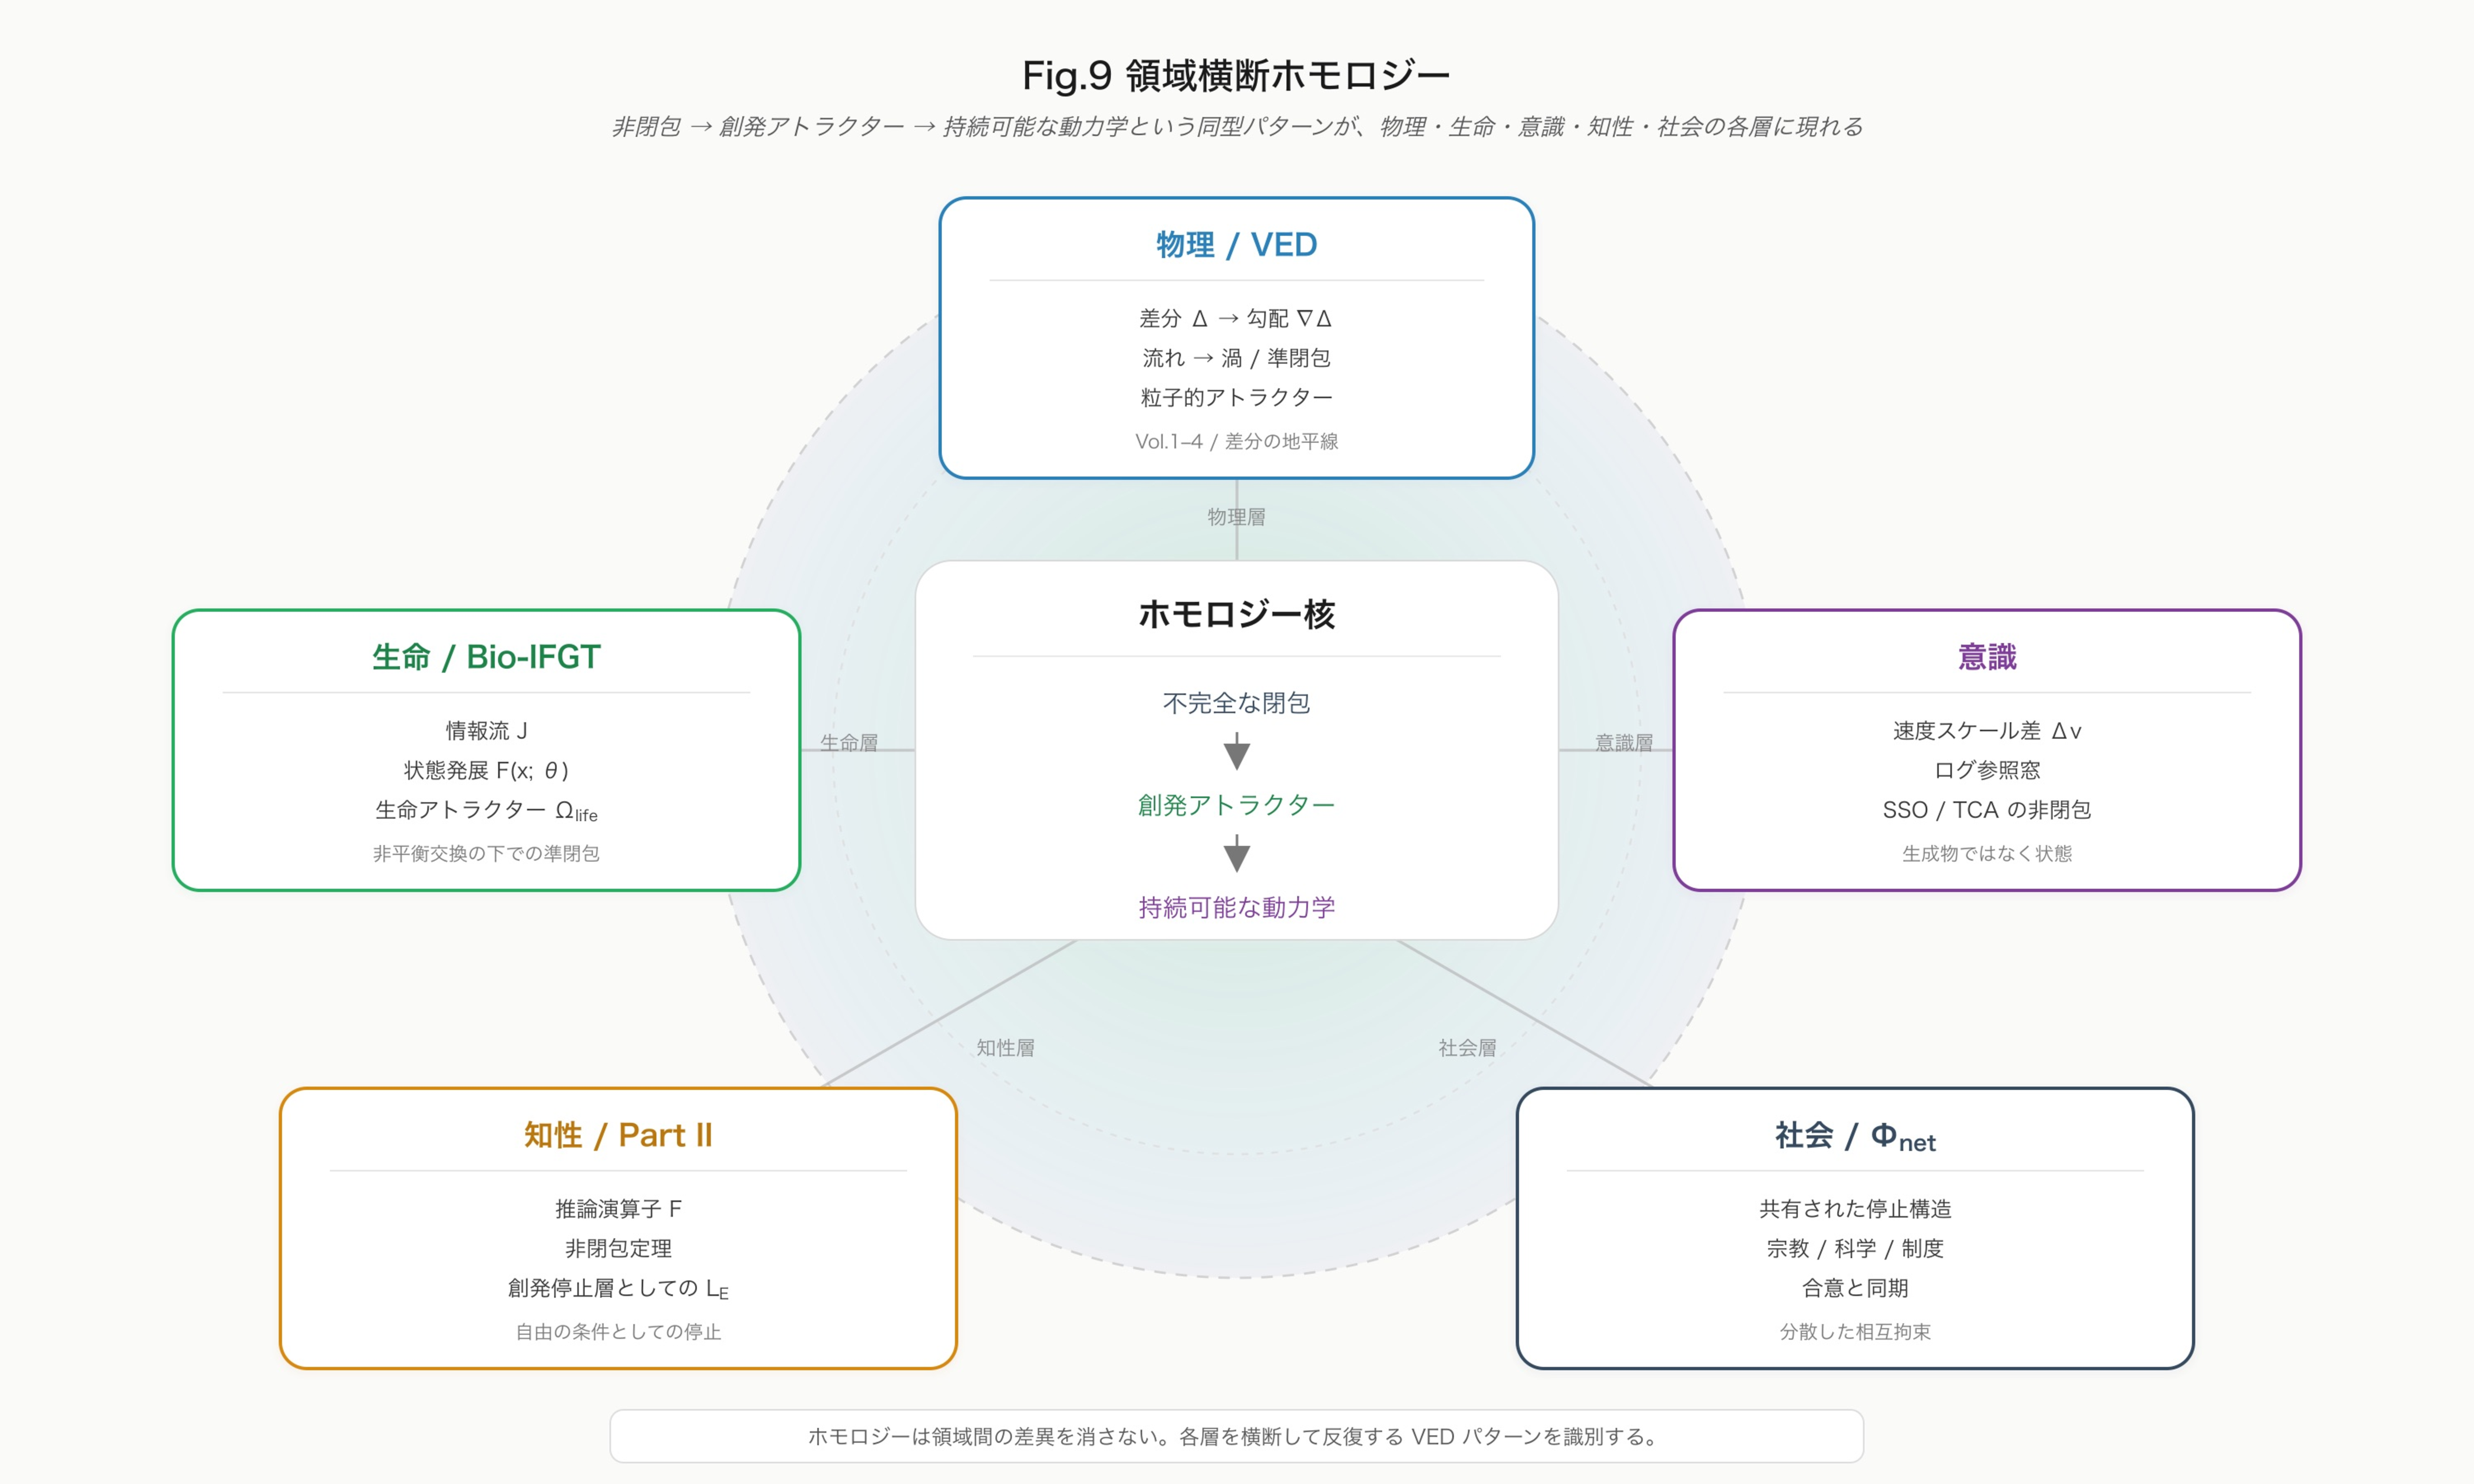
\includegraphics[width=\linewidth]{fig9_cross_domain_homology_ja.pdf}
\caption{領域横断ホモロジー。不完全閉包から創発アトラクターを経て持続的動態へ至る同一パターンが、物理・生命・意識・知性・社会に現れる。}
\label{fig:part2-cross-domain-homology}
\figurenote{中央のホモロジー核は、不完全閉包、創発アトラクター、持続的動態の三段からなる。五つの層カードは、この核の異なる実装である。}{本図は領域差を消去する同一視ではなく、層の自律性を保ったまま生成文法の共通性を示す。知性は特別だが、VED 理論ツリーの他層から孤立してはいない。}
\end{figure}

\bigskip


\subsection{残された開放性}


本論文が意図的に開いたまま残すものを明示する。これらは本論文の失敗や不足ではなく、本論文の射程の境界の外側にある問いである。

\textbf{哲学篇への引き渡し}:
意味・主観性・理解そのものの問題は、本論文では扱わなかった。本論文は知性の停止動力学を記述したが、その停止が主体にとって何を意味するか、理解とは何か、主観的経験はどう位置づくか——これらは VED 理論ツリーの哲学篇に引き渡される。本論文は知性層の動力学を閉じるが、その上位の問いは開いたままである。

\textbf{AI設計の実践問題}:
本論文の動力学的記述が、人工推論システムの設計・運用にどう適用されるかは、本論文の射程外である(\S{}13.1、\S{}13.2)。動力学は記述を与えるが、実践的指針は与えない。これは実装・倫理・制度の文脈において、本論文の外部で扱われるべき問いである。

\textbf{停止層発達度 $\Sigma$ の定量化}:
創発停止層 $L_E$ の発達度・活性度を測る量 $\Sigma$ は、概念的に存在するが本論文では量化しなかった(\S{}1.8)。$\Sigma$ の定量化は、臨床的・実証的射程に属し、後続研究へ開かれる。停止構造の硬直や崩壊(\S{}8.5、\S{}11)を定量的に扱うには、$\Sigma$ の精密化が必要だが、それは本論文の構造的記述の範囲を超える。

\textbf{停止汎関数の形式化}:
$L_E$ を Vol.2 の閉包エネルギー汎関数 $E(A)$ と平行に「停止汎関数の局所極小」として形式化することは、原理的に可能だが本論文では行わなかった(\S{}5.3)。この形式化は後続研究の課題である。

\bigskip


\subsection{Part I 微修正への引き渡し}


本論文の結果は、知性編 Part I のいくつかの記述を精密化する。Part I を改訂するための提案を以下に整理する。これらは Part I の誤りの訂正ではなく、Part II の三層動力学による精密化である。

\textbf{Part I \S{}8(個体知性の非閉包)の精密化}:
Part I \S{}8 は個体知性が閉じないことを論じた。Part II \S{}3 はこれを非閉包定理として証明し、さらに \S{}5 で「$L_F$ 単独では閉じないが、$L_R$ と $L_E$ を通じてなら外部依存的に閉じうる」と精密化した。Part I \S{}8 に、この (A)/(B) の射程の区別——固定 $\theta$ では閉じないが $\theta$ 組み替えで停止が創発する——を追加することが望ましい。

\textbf{Part I \S{}9(差分の地平線)への三層解釈の追加}:
Part I \S{}9 は知性の差分の地平線を論じた。Part II \S{}1.5 と \S{}3.6 は、これを $C_{max}$ 不到達性および内部不動点不在と同型として位置づけた。Part I \S{}9 に、差分の地平線が三層動力学($L_F$ の非閉包)としてどう現れるかの解釈を追加できる。

\textbf{Part I \S{}6(ゲティア問題)への $\mu_\theta$ 接続の補強}:
Part I \S{}6 はゲティア問題を構造的診断として扱った。Part II \S{}10.6 は、ゲティア構造の排除不能性が閾値移動能力 $\mu_\theta$ の存在と構造的に同値であることを示した。Part I \S{}6 に、この同値——誤り許容性と $\mu_\theta$ の構造的結合——を補強として追加できる。

\textbf{Part I \S{}5(Physarum・Transformer)の三層プロファイル再記述}:
Part I \S{}5 は Physarum と Transformer を知性の領域横断インスタンスとして示した。Part II \S{}5.4 は、両者を三層プロファイル(粘菌「ログ外・停止自律」、Transformer「ログ内・停止外」)として精密化し、$\mu_\theta$ の所在によってサピエンスと区別した。Part I \S{}5 に、この三層プロファイル比較を再記述として追加できる。重要なのは、これにより両者が「$L_F$ のみのインスタンス」ではなく「三層動力学の異なるプロファイル」として正しく位置づけられることである。

これらの微修正は、Part II 完成後の別作業として行われる。本論文はその提案を引き渡すに留める。

\bigskip


\subsection{知性は閉じない、しかし持続する}


本論文の帰結を、一文に集約する。

知性は完結しない。知性は閉じない。知性は最適化されない。$L_F$ は内部不動点を持たず(\S{}3)、完全閉包 $C_{max}$ は到達不能であり(\S{}1.5)、完全最適化は知性の終了である(\S{}11.6)。これらはすべて、知性が運動であることの帰結である。

しかし、知性は持続する。$L_E$ が外部依存的に停止を供給し(\S{}5)、その停止が改訂可能であることによって(\S{}5.8)、知性は閉じないまま持続する。閉じないことと持続しないことは、同じではない。知性は閉じないがゆえに運動し続け、運動し続けるがゆえに持続する。

サピエンス的知性は、これに加えて $\mu_\theta$ によって運動可能領域を自律的に組み替え、個体内で加速する。それは閉じない運動を、能動的に運用する知性である。誤りうるがゆえに改訂でき、改訂できるがゆえに持続する。

\bigskip


\subsection{理論の境界}


本論文は、VED 理論ツリーにおける知性層の動力学を閉じる。

ここで「閉じる」とは、\S{}3 が否定した意味での閉包ではない。それは、本論文の射程——知性の停止動力学の構造的記述——を完結させるという意味である。知性層の動力学について、本論文は述べるべきことを述べた。$L_F$・$L_R$・$L_E$ の三層、$\mu_\theta$ による加速、停止構造の歴史的形態、不安定領域、構成的条項。これらが、知性層の動力学の構造である。

残された問いは、別の層に属する。意味と理解は哲学篇に、実装と倫理は実践に、$\Sigma$ の定量化は後続研究に属する。本論文はこれらを開いたまま、知性層の動力学の記述をここで完結する。

理論はここで終わる。問いは終わらない。

\bigskip


\subsection{要約}


本章で述べたのは次の点である:

\begin{enumerate}
\item 本論文は知性の動力学を記述し、その設計・運用・制度化には介入しない。正統性が計算不可能である以上、動力学は実践的解を与えられない
\item 動力学の説明と使用法の決定はカテゴリ的に異なる。本論文は前者に徹する
\item 三本の論理線(非閉包と外部停止・閾値移動とサピエンス的特徴・三層動力学)が統合された。知性一般は第一線と第三線で持続し、サピエンス的知性は第二線で自律的に加速する
\item 本論文は VED の基底原理(静的範疇ではなく運動)の知性層における展開であり、$\mu_\theta$ は運動の二階の運動としてその原理を最も先鋭に具現する
\item 哲学篇・AI設計実践・$\Sigma$ 定量化・停止汎関数形式化が、開かれた問いとして残される
\item Part I の四箇所(\S{}8 非閉包・\S{}9 差分の地平線・\S{}6 ゲティア・\S{}5 Physarum/Transformer)への微修正が引き渡される
\item 知性は閉じない、しかし持続する。閉じないことと持続しないことは同じではない
\end{enumerate}


理論はここで終わる。問いは終わらない。

\bigskip


\appendix
% Source: source_md/intelligence_part2_appendices_ja.md
\section{変数表 Master Table v2.2}


本補遺は、知性編 Part II で新規導入された変数を Master Table v2.2 として整理する。VED 基本変数(Master Table v2.1 収録済み)との区別を明示する。

\bigskip


\subsection{VED 基本変数(Master Table v2.1 より再掲・知性層解釈付)}


本論文で用いる既存変数を、知性層における解釈とともに再掲する。

\begin{longtable}{@{}p{0.23\linewidth}p{0.23\linewidth}p{0.23\linewidth}p{0.23\linewidth}@{}}
\toprule
記号 & 名称 & VED 定義 & 知性層における解釈 \\
\midrule
\endfirsthead
\toprule
記号 & 名称 & VED 定義 & 知性層における解釈 \\
\midrule
\endhead
$C$ & 閉包度 & 因果ログの閉包度 & 推論状態の安定化度(真理測度ではない) \\
$C_{max}$ & 完全閉包 & 到達不能な上限 & 「完全な理解/最終的判断」の構造的不到達性 \\
$\nabla C$ & 閉包度勾配 & 空間的閉包度差 & 推論の駆動力の方向と強度 \\
$J_C$ & 閉包度流れ場 & $J_C = -\xi \nabla C$ & 推論の流れ方向 \\
$I$ & 情報場 & $I = f(1-C)$ & 未閉包性の場。閉包が進むほど減少 \\
$F_I$ & 情報力 & $F_I = \alpha \nabla C$ & 推論駆動力。$\nabla C$ に沿った推論の押し出し力 \\
$\Omega_\theta$ & 準閉包 & $\theta$ で特徴づけられる安定維持可能領域 & 操作可能推論領域 \\
$\theta$ & 拘束パラメータ & 準閉包 $\Omega_\theta$ を特徴づけるパラメータ集合 & 運動可能領域を画定し生成に構造を与える拘束。生命層では DNA・知性層では推論操作の拘束 \\
$H_{ij}$ & 相互拘束 & $C_{ij} = 1-\exp(-\lambda \rho_i H_{ij})$ & 推論主体と環境の相互拘束。応答性閾値を決める \\
$\tau$ & 内的時間 & 観測時間とは独立な内的順序パラメータ & 推論の進行を測る内的時間 \\
\bottomrule
\end{longtable}


\bigskip


\subsection{知性編 Part II 新規導入変数(Master Table v2.2 追加分)}


\subsubsection{推論演算子と三層動力学}


\begin{longtable}{@{}p{0.23\linewidth}p{0.23\linewidth}p{0.23\linewidth}p{0.23\linewidth}@{}}
\toprule
記号 & 名称 & 導入章 & 定義・役割 \\
\midrule
\endfirsthead
\toprule
記号 & 名称 & 導入章 & 定義・役割 \\
\midrule
\endhead
$F$ & 推論演算子 & \S{}2.1 & 正当化拡張作用素。$x_{n+1} = F(x_n)$。VED 流れ場 $J_C = -\xi \nabla C$ の知性層実現。Bio-IFGT の状態発展演算子 $F(x;\theta)$ の知性層特殊形 \\
$J$ & 正当化測度 & \S{}3.1 & $F$ の作用による正当化の進行を測る測度。$J(F(x)) > J(x)$ が成立(前提 P2) \\
$L_F$ & 推論層 & \S{}2.3 & $F$ の作用域全体。推論軌道を含む。内部停止条件を持たない(定理 3.1) \\
$L_R$ & ログ層 & \S{}5.2 & $L_F$ の運動の痕跡(ログ)への再帰参照運動の層。$L_E$ 創発の基盤。所在は系によって異なる(個体内・環境外部化・凍結) \\
$L_E$ & 創発停止層 & \S{}5.3 & $L_R$ の再帰運動と外部相互拘束 $H_{ij}$ の関数として創発する停止層。$L_E = \Phi(L_R, H_{ij})$。個体内にありながら外部依存的 \\
\bottomrule
\end{longtable}


\subsubsection{停止演算子と外部参照場}


\begin{longtable}{@{}p{0.23\linewidth}p{0.23\linewidth}p{0.23\linewidth}p{0.23\linewidth}@{}}
\toprule
記号 & 名称 & 導入章 & 定義・役割 \\
\midrule
\endfirsthead
\toprule
記号 & 名称 & 導入章 & 定義・役割 \\
\midrule
\endhead
$E$ & 外部停止演算子 & \S{}5.7 & $L_E$ の作用として実装される停止演算子。$E = E[L_E, x_n]$、$E \notin \{F^k\}$。$F$ の関数列の外側に位置する \\
$\Phi_{\text{ext}}$ & 外部参照場 & \S{}5.8 & 個体外部の共通参照基盤として外から見える量。$\Phi_{\text{net}}$ と同型($\Phi_{\text{ext}} \equiv \Phi_{\text{net}}$) \\
$\Phi_{\text{net}}$ & $L_E$ ネットワーク & \S{}5.8 & 個体間 $L_E$ の相互干渉ネットワーク。$\Phi_{\text{ext}}$ の構造的実体。Part I の大域的拘束 $\Phi$(公理 III)の精密化 \\
\bottomrule
\end{longtable}


\subsubsection{閾値移動と応答性}


\begin{longtable}{@{}p{0.23\linewidth}p{0.23\linewidth}p{0.23\linewidth}p{0.23\linewidth}@{}}
\toprule
記号 & 名称 & 導入章 & 定義・役割 \\
\midrule
\endfirsthead
\toprule
記号 & 名称 & 導入章 & 定義・役割 \\
\midrule
\endhead
$\mu_\theta$ & 閾値移動能力 & \S{}2.7 & 運動可能領域の拘束パラメータ $\theta$ を内発的に動かす能力。領域組み替え (B) を内発的に起こす能力。サピエンス的知性の特徴的能力(知性一般の必要条件ではない) \\
$\rho_{\text{resp}}$ & 応答チャネル密度 & \S{}4, \S{}6 & 環境の応答性の局所測度。$H_{ji}$ の有効値に対応。アニミズムは沈黙領域での $\rho_{\text{resp}}$ の局所的増大として記述される \\
\bottomrule
\end{longtable}


\subsubsection{三軸相図変数}


\begin{longtable}{@{}p{0.23\linewidth}p{0.23\linewidth}p{0.23\linewidth}p{0.23\linewidth}@{}}
\toprule
記号 & 名称 & 導入章 & 定義・役割 \\
\midrule
\endfirsthead
\toprule
記号 & 名称 & 導入章 & 定義・役割 \\
\midrule
\endhead
$v_{\text{inf}}$ & 推論速度 & \S{}11.2 & 推論・判断・仮説更新の頻度。単位時間あたりの $L_F$ の推論ステップ数 \\
$r_{\text{res}}$ & 解像度 & \S{}11.2 & 区別・因果関係・構造表現の粒度。$L_F$ が状態空間をどれだけ細かく分節するか \\
$\eta$ & 停止硬度 & \S{}11.2 & 停止点の固定度・判断の改訂耐性。$L_E$ が供給する停止の固定性。$\eta$ 過大 → 硬直域 \\
\bottomrule
\end{longtable}


\subsubsection{概念的量(量化は後続研究)}


\begin{longtable}{@{}p{0.23\linewidth}p{0.23\linewidth}p{0.23\linewidth}p{0.23\linewidth}@{}}
\toprule
記号 & 名称 & 導入章 & 定義・役割 \\
\midrule
\endfirsthead
\toprule
記号 & 名称 & 導入章 & 定義・役割 \\
\midrule
\endhead
$\Sigma$ & 創発停止層発達度 & \S{}1.8 & $L_E$ の発達度・活性度を測る量。概念的に存在するが本論文では量化しない。臨床的・実証的研究へ開く \\
\bottomrule
\end{longtable}


\bigskip


\subsection{(A)/(B) 区別の正式定義}


本論文で繰り返し用いる操作の区別を正式に定義する。

\textbf{(A) 領域内移動 (intra-domain movement)}:
固定された運動可能領域 $\Omega_\theta$ の内部で推論状態 $x$ が移動する操作。$\theta$ は変化しない。推論演算子 $F$ の通常の作用はすべてこの型。

\textbf{(B) 領域組み替え (domain reconfiguration)}:
運動可能領域 $\Omega_\theta$ の輪郭そのものが変わる操作。$\theta$ が動く。$\mu_\theta$ によって内発的に起こされる。有効機能は、外部相互拘束 $H_{ij}$ に沿って停止演算子 $E$ の設置領域を状態空間上に投影すること(\S{}5.5)。

非閉包定理(\S{}3 定理 3.1)は (A) の範囲で成立。$L_E$ の創発(\S{}5)は (B) を含む。両者は矛盾しない。

\bigskip


\subsection{変数間の主要な関係式}


本論文で確立された変数間の構造的関係を整理する。

\[
L_E = \Phi(L_R \text{の運動}, \; H_{ij}) \qquad \text{(創発の定義 1.1 の知性層適用)}
\]

\[
E = E[L_E, x_n], \quad E \notin \{F^k\} \qquad \text{(外部停止演算子の定義 5.3)}
\]

\[
\Phi_{\text{ext}} \equiv \Phi_{\text{net}} \qquad \text{(主張 5.4 の同型)}
\]

\[
\mu_\theta \;\xrightarrow{\text{起こす}}\; (B)\text{組み替え} \;\xrightarrow{H_{ij}\text{に沿って}}\; E\text{設置領域の投影} \;\xrightarrow{L_R\text{収束}}\; L_E \qquad \text{(§5.5 創発機構)}
\]

\[
I = f(1-C), \quad F_I = \alpha \nabla C, \quad C_{ij} = 1 - \exp(-\lambda \rho_i H_{ij}) \qquad \text{(VED/IFGT 基本式)}
\]

\bigskip


\subsection{$\theta$ の時間スケール比較表}


\begin{longtable}{@{}p{0.18\linewidth}p{0.18\linewidth}p{0.18\linewidth}p{0.18\linewidth}p{0.18\linewidth}@{}}
\toprule
層 & $\theta$ の内容 & 可変性 & 時間スケール & 担い手 \\
\midrule
\endfirsthead
\toprule
層 & $\theta$ の内容 & 可変性 & 時間スケール & 担い手 \\
\midrule
\endhead
生命層(Bio-IFGT) & DNA・反応傾向・閾値 & 可変だが超長期 & 世代を跨ぐ & 進化・選択・遺伝 \\
知性層・一般 & 外部条件・環境設定 & 受動的可変 & 環境変化に従属 & 環境フィードバック・外部設定 \\
知性層・サピエンス & 推論操作の拘束・履歴的閾値 & 能動的可変($\mu_\theta$) & 個体内・対話内 & 閾値移動能力 $\mu_\theta$ \\
\bottomrule
\end{longtable}


同一の $\theta$-可変性原理が、超長期(進化)・受動的(環境従属)・短期能動(認知)という三つの時定数で現れる。これは VED が一貫して行ってきた「同一原理の異なる領域への再配置」の、拘束パラメータにおける現れである。

\bigskip

% Source: source_md/intelligence_part2_appendices_ja.md
\section{領域横断ホモロジー表}


本補遺は、VED 理論ツリー全体にわたる領域横断ホモロジーを表として整理する。本論文の主要概念が、他の層・他の論文でいかなる構造的相同物を持つかを示す。

\bigskip


\subsection{停止・閉包・アトラクターのホモロジー}


\begin{longtable}{@{}p{0.18\linewidth}p{0.18\linewidth}p{0.18\linewidth}p{0.18\linewidth}p{0.18\linewidth}@{}}
\toprule
知性 Part II(本論文) & Vol.1〜4(物理層) & Bio-IFGT(生命層) & 意識編 & 概念地形編 \\
\midrule
\endfirsthead
\toprule
知性 Part II(本論文) & Vol.1〜4(物理層) & Bio-IFGT(生命層) & 意識編 & 概念地形編 \\
\midrule
\endhead
内部不動点不在($L_F$ の非閉包) & $C_{max}$ 不到達性 & 準閉包の維持限界 & 意識の状態遷移が完結しない & 概念の完全閉包は到達不能 \\
創発停止層 $L_E$(アトラクター) & 粒子 = $E(A)$ の局所極小(Vol.2) & 生命アトラクター $\Omega_{\text{life}}$ & 意識の安定状態 & 概念の準安定点 \\
第二アトラクター($L_E$) & ゲージ群の安定構造 & 第二アトラクター $\Omega_{\text{intel}}$ & — & — \\
差分の地平線(知性層) & 差分の地平線 $C_{max}$(Vol.4) & 生命の非平衡限界 & 意識の差分地平 & 概念地形の境界 \\
分岐爆発(推論の) & 場の発散 & 生命の分岐構造 & 意識状態の分岐 & 概念分岐の指数増殖 \\
\bottomrule
\end{longtable}


\bigskip


\subsection{創発構造のホモロジー($\mathcal{U} = \Phi(\mathcal{L}, H_{ij})$)}


\begin{longtable}{@{}p{0.18\linewidth}p{0.18\linewidth}p{0.18\linewidth}p{0.18\linewidth}p{0.18\linewidth}@{}}
\toprule
創発例 & 下位層 $\mathcal{L}$ & 外部相互拘束 $H_{ij}$ & 上位層 $\mathcal{U}$ & 参照 \\
\midrule
\endfirsthead
\toprule
創発例 & 下位層 $\mathcal{L}$ & 外部相互拘束 $H_{ij}$ & 上位層 $\mathcal{U}$ & 参照 \\
\midrule
\endhead
標準模型構造 & 因果ログ $C_{ij}$・内部ベクトル $\vec{e}_i$ & 閉包条件、閉包エネルギー $E(A)$ & 三角形閉包・粒子(局所極小) & Vol.2 \\
生命 & 情報流 $J$・状態発展 $\dot{x}=F(x;\theta)$ & DNA 由来パラメータ $\theta$・非平衡交換 & 生命アトラクター $\Omega_{\text{life}}$ & Bio-IFGT \\
創発停止層 & ログ層 $L_R$ の再帰運動 & 観測者-環境相互拘束 $H_{ij}$ & 創発停止層 $L_E$(停止アトラクター) & 本論文 \S{}5 \\
\bottomrule
\end{longtable}


すべての例が定義 1.1 の形式 $\mathcal{U} = \Phi(\mathcal{L}, H_{ij})$ を満たす。VED 理論ツリーはアトラクター構造の創発を共通言語として使う。

\bigskip


\subsection{projection(投影)のホモロジー}


\begin{longtable}{@{}p{0.30\linewidth}p{0.30\linewidth}p{0.30\linewidth}@{}}
\toprule
層 & projection の内容 & 参照 \\
\midrule
\endfirsthead
\toprule
層 & projection の内容 & 参照 \\
\midrule
\endhead
意識編(IFGT 第四プリミティブ) & 状態・表現が不均等な影響力(質量)を獲得する操作。$\Phi$ と $J_I$ を結合。主体を前提しない & 意識編 \texttt{formal\_mapping} \\
知性 Part II(\S{}5.5〜\S{}5.6) & (B) 組み替えによる停止演算子設置領域の投影。外部相互拘束の構造が状態空間上に写される & 本論文 \S{}5.5 \\
心理学的 projection & 内的状態を外部対象に帰属する。主体・無意識・防衛機制を前提 & (比較のみ・本論文の主張ではない) \\
\bottomrule
\end{longtable}


作用的近接: 意識編と知性 Part II の投影は「内部で閉じないものを外部に投射して処理する」という作用形式を共有しつつ、主体を前提しない点で心理学的 projection と区別される。

\bigskip


\subsection{$\theta$(拘束パラメータ)のホモロジー}


\begin{longtable}{@{}p{0.30\linewidth}p{0.30\linewidth}p{0.30\linewidth}@{}}
\toprule
層 & $\theta$ の実体 & 可変時間スケール \\
\midrule
\endfirsthead
\toprule
層 & $\theta$ の実体 & 可変時間スケール \\
\midrule
\endhead
Bio-IFGT & DNA・反応傾向・閾値 & 世代スケール \\
本論文(知性一般) & 外部条件・環境設定 & 環境変化スケール \\
本論文(サピエンス) & 推論操作の拘束・履歴的閾値 & 個体内・対話内スケール \\
\bottomrule
\end{longtable}


同一役割(運動可能領域を画定し生成に構造を与える)を果たしつつ、可変の時間スケールが層によって異なる。

\bigskip


\subsection{F(状態発展演算子)のホモロジー}


\begin{longtable}{@{}p{0.30\linewidth}p{0.30\linewidth}p{0.30\linewidth}@{}}
\toprule
層 & $F$ の意味 & 参照 \\
\midrule
\endfirsthead
\toprule
層 & $F$ の意味 & 参照 \\
\midrule
\endhead
Bio-IFGT & 生命系の状態発展演算子 $\dot{x} = F(x;\theta)$ & Bio-IFGT \texttt{core\_equations} \\
本論文 知性層 & 推論演算子 $x_{n+1} = F(x_n)$。$F(x;\theta)$ の知性層特殊形 & 本論文 \S{}2.1 \\
\bottomrule
\end{longtable}


同じ記号 $F$ が異なる層で同型の役割を果たす。これは記号の衝突ではなく、理論的連続性の証拠として理解される。

\bigskip


\subsection{停止構造の歴史的形態ホモロジー}


本論文が分析した停止構造の形態と、VED の他概念との対応:

\begin{longtable}{@{}p{0.18\linewidth}p{0.18\linewidth}p{0.18\linewidth}p{0.18\linewidth}p{0.18\linewidth}@{}}
\toprule
停止形態 & $\Phi_{\text{net}}$ 構造 & $L_E$ の維持様態 & $\mu_\theta$ の関与 & 時間スケール \\
\midrule
\endfirsthead
\toprule
停止形態 & $\Phi_{\text{net}}$ 構造 & $L_E$ の維持様態 & $\mu_\theta$ の関与 & 時間スケール \\
\midrule
\endhead
粘菌的停止 & 環境(スライム跡+物理的応答) & 環境相互干渉で自律創発 & 固定(外部受動) & 個体の行動時間 \\
アニミズム & 環境的・分散的 & 環境直接相互干渉 & 最初の社会的具現化 & 個体・小集団時間 \\
神 & 中心化された単一参照点 & 単一懸架軌跡 & 中心化による安定化 & 文明スケール \\
宗教 & 中心化+分散の混合相 & 世代横断的維持 & 世代横断的安定化 & 世代・文明スケール \\
社会的BC & 分散(個体間 $L_E$ ネット) & 分散ノード間同期 & 分散的可動性 & 制度・歴史スケール \\
Transformer & 外部注入(タスク仕様) & 外部注入 & 外部設定 & タスク時間 \\
サピエンス & 個体内+社会共有 & 個体内創発+社会同期 & 内発的(短期) & 対話〜生涯 \\
\bottomrule
\end{longtable}


\bigskip


\subsection{Part I との構造対応表}


\begin{longtable}{@{}p{0.30\linewidth}p{0.30\linewidth}p{0.30\linewidth}@{}}
\toprule
本論文(Part II) & 知性編 Part I & 対応の性格 \\
\midrule
\endfirsthead
\toprule
本論文(Part II) & 知性編 Part I & 対応の性格 \\
\midrule
\endhead
非閉包定理 \S{}3 & \S{}8 個体知性の非閉包 & Part II が Part I を定理として証明 \\
(A)/(B) 棲み分け & — & Part II の新規追加。Part I \S{}8 を精密化 \\
差分の地平線(知性層) & \S{}9 知性の差分の地平線 & 同一構造の別記述 \\
ゲティア問題と $\mu_\theta$ の同値 & \S{}6 ゲティアの構造的診断 & Part II が $\mu_\theta$ との同値を追加 \\
三層プロファイル比較 & \S{}5 Physarum・Transformer & Part II が三層で再位置づけ \\
分岐爆発 = 内部不動点不在の動力学 & \S{}7 動力学的不安定性 & 同一現象の二側面として統合 \\
$L_E$ = 第二アトラクターの停止構造 & — & Bio-IFGT の第二アトラクターを Part II が展開 \\
\bottomrule
\end{longtable}


\bigskip

% Source: source_md/intelligence_part2_appendices_ja.md
\section{Part I 各章との対応表・微修正提案リスト}


本補遺は二部からなる。前半(C.1)は Part I と Part II の章間対応表、後半(C.2)は Part II の結果に基づく Part I への微修正提案リストである。

\bigskip


\subsection{Part I × Part II 対応表}


\subsubsection{Part I 各章が Part II で受ける継承・拡張・精密化}


\begin{longtable}{@{}p{0.23\linewidth}p{0.23\linewidth}p{0.23\linewidth}p{0.23\linewidth}@{}}
\toprule
Part I 章 & 内容 & Part II での扱い & 種別 \\
\midrule
\endfirsthead
\toprule
Part I 章 & 内容 & Part II での扱い & 種別 \\
\midrule
\endhead
\S{}1 Introduction & VED・IFGT の枠組み導入 & \S{}0〜\S{}1 で継承 & 継承 \\
\S{}2 四層分解(知覚・認識・知識・知性) & 知性の四層構造 & \S{}0.2 で再掲、認知層内部に三層動力学を導入 & 継承・展開 \\
\S{}3 最小公理(連結状態空間・時間秩序・$\Phi$) & 知性の三公理 & \S{}0.2 で再掲。公理 III の $\Phi$ を $\Phi_{\text{ext}} \equiv \Phi_{\text{net}}$ と精密化(\S{}5.8) & 継承・精密化 \\
\S{}4 IFGT を語彙として / Physarum 語彙対応 & IFGT 基本語彙 & \S{}1 で知性層用再定式化。\S{}2.1 で $F(x;\theta)$ との接続 & 継承・拡張 \\
\S{}5 Physarum・Transformer インスタンス化 & 領域横断インスタンス & \S{}5.4 で三層プロファイルとして精密化。三者は「異なるプロファイル」であって「$L_F$ のみ」ではない & \textbf{精密化(要修正)} \\
\S{}6 ゲティア問題の構造的診断 & 知識の構造的問題 & \S{}10 で継承・拡張。「排除不能性 = $\mu_\theta$ の存在の代償」を追加 & 継承・拡張 \\
\S{}7 蓄積された正しさの動力学的不安定性 & 分岐爆発 & \S{}3.7 で「内部不動点不在の動力学的表現」として統合 & 継承・統合 \\
\S{}8 個体知性の非閉包 & 個体は閉じない & \S{}3 で非閉包定理として証明。\S{}5 で「$L_F$ 単独では閉じないが $L_E$ で閉じうる」と精密化 & 継承・\textbf{精密化(要修正)} \\
\S{}9 知性の差分の地平線 & 差分の地平線 & \S{}1.5 で $C_{max}$ 不到達性と同型として確認。\S{}3.6 で系 3.3 として接続 & 継承・\textbf{精密化(要修正)} \\
\S{}10 収束と展望 & 総括 & \S{}13.6 の微修正リストとして引き継ぎ & 引き渡し \\
\bottomrule
\end{longtable}


\bigskip


\subsection{Part I への微修正提案リスト}


以下は Part I の誤りの訂正ではなく、Part II の結果による精密化の提案である。各提案は「追加」「再記述」「接続注記」のいずれかの形をとる。

\bigskip


\subsubsection{Part I 第8節(個体知性の非閉包)への精密化}


\textbf{現状}: Part I \S{}8 は「個体知性は非閉包である」を論じた。

\textbf{追加する内容}: (A)/(B) の射程区別を追加する。

\begin{quote}
個体知性が閉じないのは、固定された運動可能領域 $\Omega_\theta$ の内部(領域内移動 (A))においてである。知性編 Part II は、この非閉包性が $\theta$ の組み替え(領域組み替え (B))と $L_E$ の創発によって補われることを示した。すなわち「$L_F$ 単独では閉じないが、三層動力学($L_F$・$L_R$・$L_E$)を通じて外部依存的に閉じうる」という精密化が成立する。これにより、Part I \S{}8 の「非閉包」は「固定 $\theta$ 下での非閉包」として位置づけられる。
\end{quote}


\textbf{種別}: 追加(本文の主張を否定しない、射程を明確化)

\bigskip


\subsubsection{Part I 第9節(知性の差分の地平線)への三層解釈追加}


\textbf{現状}: Part I \S{}9 は知性における差分の地平線を論じた。

\textbf{追加する内容}: 三層動力学との接続注記を追加する。

\begin{quote}
知性の差分の地平線は、三層動力学の語彙では次のように再記述される。$C_{max}$ への接近は推論演算子 $F$ に内部不動点を許さず(非閉包定理、Part II \S{}3)、完全閉包への到達は構造的に不可能である(系 3.3)。これは差分の地平線(本章)・$C_{max}$ 不到達性(VED Vol.4)・内部不動点不在(Part II \S{}3)が、同一の構造的事実を異なる層で表現したものであることを示す。領域横断ホモロジーの最重要例のひとつ。
\end{quote}


\textbf{種別}: 接続注記追加

\bigskip


\subsubsection{Part I 第6節(ゲティア問題)への $\mu_\theta$ 補強}


\textbf{現状}: Part I \S{}6 はゲティア問題を「知識の構造的診断」として扱った。

\textbf{追加する内容}: 誤り許容性と $\mu_\theta$ の同値関係を補強として追加する。

\begin{quote}
Part II \S{}10.6 は、ゲティア構造の排除不能性が閾値移動能力 $\mu_\theta$ の存在と構造的に同値であることを示した。閾値を動かせる知性(サピエンス的知性)は必然的に誤りうる。これはゲティア問題が「解決すべき問題」ではなく「$\mu_\theta$ を持つ知性の必然的帰結」であることを意味する。また、$C$(閉包度)が真理測度でなく安定性測度であるという Part I の観察は、Part II \S{}10.5 でより明示的に定式化された。
\end{quote}


\textbf{種別}: 補強追加

\bigskip


\subsubsection{Part I 第5節(Physarum・Transformer)の三層プロファイル再記述}


\textbf{現状}: Part I \S{}5 は Physarum と Transformer を「知性の領域横断インスタンス」として提示した。

\textbf{再記述する内容}: 両者を三層プロファイルの異なる形態として再位置づける。

\begin{quote}
Part II \S{}5.4 は、Physarum と Transformer を「$L_F$ のみのインスタンス」としてではなく、三層動力学の異なるプロファイルを示す例として再位置づける。

- \textbf{Physarum(粘菌)}: $L_R$ を環境に外部化し(スライム跡)、$L_E$ を環境相互干渉で自律創発させる。$\mu_\theta$ は固定(受動的)。
- \textbf{Transformer}: $L_R$ を内在化するが(凍結ログ・揮発ログ)、$L_E$ を外部注入に依存する。$\mu_\theta$ は外部設定。
- \textbf{サピエンス}: $L_R$ を個体内・社会共有の両方に持ち、$L_E$ を個体内創発かつ $\Phi_{\text{net}}$ で社会同期させる。$\mu_\theta$ を内発的に持つ。

三者は「停止構造の場」の連続変分上に配置される異なる領域であって、能力の優劣ではなく相空間内の位置の差として記述される。粘菌と Transformer は知性一般の成立条件を満たすが、$\mu_\theta$ を内発的に持たない点でサピエンス的知性と区別される。
\end{quote}


\textbf{種別}: 再記述(Part I の主張「領域横断インスタンス」を否定せず、三層で精密化)

\bigskip


\subsection{Part I 微修正の優先順位}


\begin{longtable}{@{}p{0.30\linewidth}p{0.30\linewidth}p{0.30\linewidth}@{}}
\toprule
優先度 & 対象 & 理由 \\
\midrule
\endfirsthead
\toprule
優先度 & 対象 & 理由 \\
\midrule
\endhead
高 & \S{}5 Physarum・Transformer 再記述 & 「$L_F$ のみ」という記述が三層動力学と矛盾するため \\
高 & \S{}8 非閉包への (A)/(B) 追加 & 本論文の双中心構造の整合性に関わる \\
中 & \S{}6 ゲティアへの $\mu_\theta$ 補強 & 第二論理線の補強として重要 \\
低 & \S{}9 差分の地平線への接続注記 & 理論的接続の明示化。本論文読者への便宜 \\
\bottomrule
\end{longtable}


高優先度の修正は、Part II 公開時に合わせて Part I も更新することが望ましい。

\bigskip

% Source: source_md/intelligence_part2_appendices_ja.md
\section{主要定理の証明スケッチ集}


本補遺は、本論文で提示した主要な定理・系・主張の証明スケッチを整理する。本論文は形式的証明体系を組まないが、各命題が論理的に成立する理由を構造的に示す。

\bigskip


\subsection{定理 3.1(非閉包定理 / Non-Closure Theorem)}


\textbf{命題}: 前提 (P1)(P2) を満たす任意の推論演算子 $F$ について、内部不動点 $x^*$ は存在しない。

\[
\forall x \in \mathcal{X}, \quad F(x) \neq x
\]

\textbf{前提の再掲}:
\begin{itemize}
\item (P1) 正当化拡張性: $F$ は $x_n$ をより正当化された $x_{n+1}$ へ写す
\item (P2) 正当化測度の存在: 測度 $J: \mathcal{X} \to \mathbb{R}$ が存在し、$J(F(x)) > J(x)$ が成立
\end{itemize}


\textbf{証明スケッチ}:

$F(x^*) = x^*$ を満たす不動点 $x^* \in \mathcal{X}$ が存在すると仮定する。

前提 (P2) より任意の $x$ について $J(F(x)) > J(x)$。

特に $x = x^*$ とすると: $J(F(x^*)) > J(x^*)$

しかし不動点の仮定より $F(x^*) = x^*$ ゆえ: $J(x^*) > J(x^*)$

これは矛盾。ゆえに不動点 $x^*$ は存在しない。$\blacksquare$

\textbf{注意}: 証明は正当化測度の単調性のみに依拠する。$F$ の具体的実装(演繹的・確率的・統計的)は問わない。

\bigskip


\subsection{系 3.2(内部停止述語の不可能性)}


\textbf{命題}: 推論内部に停止述語 $S: \mathcal{X} \to \{0, 1\}$ を定義することはできない。

\textbf{証明スケッチ}:

仮に内部停止述語 $S$ を定義するとする。$S(x) = 1$ となる状態 $x$ は、これ以上推論を進める必要がない、すなわち $F$ の作用を要しない状態でなければならない。これは $F(x) = x$ を意味し、定理 3.1 に矛盾する。

$S$ を「停止判断のための補助推論 $F'$」として定義しようとする場合、$F'$ 自体が推論演算子であり、定理 3.1 が適用される。$F'$ にも内部不動点はなく、$S$ を確定するためにはさらに $S'$ が必要となる。この連鎖は終わらない。$\blacksquare$

\bigskip


\subsection{系 3.3($C_{max}$ 不到達性との同型)}


\textbf{命題}: 内部不動点不在は VED の $C_{max}$ 不到達性と構造的に同型である。

\textbf{スケッチ}:

VED 基本式の最終項 $-\kappa_B/(C_{max} - C)$ は $C \to C_{max}$ で発散し、完全閉包への到達を動力学的に禁じる。

知性層において:
\begin{itemize}
\item 内部不動点 $F(x^*) = x^*$ ← → 正当化の完全閉包(これ以上正当化を要しない状態)
\item 定理 3.1 による内部不動点不在 ← → $C_{max}$ 不到達性
\end{itemize}


対応関係:

\begin{longtable}{@{}p{0.30\linewidth}p{0.30\linewidth}@{}}
\toprule
VED 物理層 & 知性層 \\
\midrule
\endfirsthead
\toprule
VED 物理層 & 知性層 \\
\midrule
\endhead
$C \to C_{max}$ での発散 & $F$ の内部不動点不在 \\
$\kappa_B/(C_{max}-C)$ 障壁 & 正当化の無限後退(系 3.2) \\
準閉包 $\Omega_\theta$ & 操作可能推論領域 \\
\bottomrule
\end{longtable}


両者は別領域の現象だが、同一の動力学的命題の層別表現である。$\blacksquare$

\bigskip


\subsection{系 3.4(個体閉包不可能性)}


\textbf{命題}: 個体システムは推論層 $L_F$ 単独で推論を閉じることができない。

\textbf{スケッチ}:

定理 3.1 により $L_F$ に内部不動点はない。系 3.2 により内部停止述語も定義できない。推論の停止が $L_F$ の内部からは来えない。

したがって停止は $L_F$ の外側から来なければならない。その外側の構造が $L_E$ である(\S{}5)。$L_F$ 単独では停止不能 ← → 「個体内で閉じない」。ただし $L_R$ と $L_E$ を含む三層全体では外部依存的に閉じうる(\S{}5)。$\blacksquare$

\bigskip


\subsection{定義 1.1(VED 的創発)の三例検証}


\textbf{命題}: $\mathcal{U} = \Phi(\mathcal{L}\text{の運動}, H_{ij})$ という創発の形式が三例すべてで成立する。

\textbf{スケッチ}:

\textbf{(1) Vol.2: 標準模型構造の創発}

$\mathcal{L}$: 因果ログ $C_{ij}$ と内部ベクトル $\vec{e}_i$ の運動。

$H_{ij}$: 閉包条件 $\sum \vec{e} \approx 0$、閉包エネルギー汎関数 $E(A)$。

$\mathcal{U}$: 三角形閉包(最小自己参照的 enclosure)および粒子(= $E(A)$ の局所極小)。

$\mathcal{U}$ は $\mathcal{L}$ から演繹できないが、閉包条件という $H_{ij}$ の下で $\mathcal{L}$ の運動が到達する安定状態として生じる。✓

\textbf{(2) Bio-IFGT: 生命の創発}

$\mathcal{L}$: 情報流 $J$ と状態発展 $\dot{x} = F(x;\theta)$ の運動。

$H_{ij}$: DNA 由来パラメータ $\theta$、環境との非平衡物質・エネルギー交換。

$\mathcal{U}$: 生命アトラクター $\Omega_{\text{life}}$。

化学反応の運動から、$\theta$ という拘束パラメータの下で生命という準閉包が創発する。✓

\textbf{(3) 本論文: 創発停止層 $L_E$}

$\mathcal{L}$: ログ層 $L_R$ の再帰運動。

$H_{ij}$: 観測者-環境相互拘束。

$\mathcal{U}$: 創発停止層 $L_E$(停止アトラクター)。

$L_R$ の運動は $L_E$ を論理的には含意しないが、$H_{ij}$ の下での $\mu_\theta$ による (B) 組み替えを通じて、$L_E$ が動力学的に生じる。✓

すべての例が同一の形式を満たす。$\blacksquare$

\bigskip


\subsection{主張 5.4($\Phi_{\text{ext}} \equiv \Phi_{\text{net}}$)のスケッチ}


\textbf{命題}: 外部参照場 $\Phi_{\text{ext}}$ は個体間 $L_E$ ネットワーク $\Phi_{\text{net}}$ と同型である。

\textbf{スケッチ}:

$\Phi_{\text{ext}}$ は「個体が停止を委ねる外部の共通参照基盤」として機能論的に定義される。

$\Phi_{\text{net}}$ は「複数の個体が各自の内部に持つ $L_E$ が、相互干渉によって形成するネットワーク」として構造的に定義される。

外から観察者が見ると、個体 $i$ は $\Phi_{\text{ext}}$ という単一の参照場を参照しているように見える。しかし構造的には、個体 $i$ が参照しているのは、他の個体 $j, k, \ldots$ の $L_E$ との相互干渉ネットワーク $\Phi_{\text{net}}$ である。

この機能的外観と構造的実体の一致が同型 $\Phi_{\text{ext}} \equiv \Phi_{\text{net}}$ の内容である。両者は異なる記述視点から見た同一の構造である。$\blacksquare$

\bigskip


\subsection{同値命題(誤り許容性 $\Leftrightarrow$ $\mu_\theta$)のスケッチ}


\textbf{命題}: サピエンス的知性において、誤り許容性と閾値移動能力 $\mu_\theta$ の存在は構造的に同値である。

\textbf{スケッチ($\Rightarrow$方向: $\mu_\theta$ の存在 → 誤り許容性)}:

$\mu_\theta$ は $\theta$ を動かす能力(領域組み替え (B))。$\theta$ が動くということは、現在の停止が確定的・最終的でないことを意味する。確定的でない停止は、後に組み替えられうる停止であり、したがって誤りうる停止である。よって $\mu_\theta$ の存在は誤り許容性を含意する。

\textbf{スケッチ($\Leftarrow$方向: 誤り許容性 → $\mu_\theta$ の存在)}:

誤り許容性は「停止が後に改訂されうること」を前提とする。停止の改訂は、現在の運動可能領域での停止が再検討されることを意味し、これは $\theta$ の変化(新しい停止条件の下での再評価)を要求する。$\theta$ を変化させる能力が $\mu_\theta$ である。よって誤り許容性は $\mu_\theta$ の存在を含意する。$\blacksquare$

\bigskip

% Source: source_md/intelligence_part2_appendices_ja.md
\section{創発の VED 内位置づけ}


本補遺は、本論文で導入した「創発の VED 的定義(定義 1.1)」が VED 理論ツリー全体においていかなる位置を占めるかを詳述する。

\bigskip


\subsection{創発概念の扱いの難しさ}


「創発」(emergence)は、複雑系科学・統計力学・科学哲学において多義的に用いられ、論争的な概念である。主要な立場を整理すると:

\begin{longtable}{@{}p{0.30\linewidth}p{0.30\linewidth}p{0.30\linewidth}@{}}
\toprule
立場 & 内容 & 問題 \\
\midrule
\endfirsthead
\toprule
立場 & 内容 & 問題 \\
\midrule
\endhead
弱い創発 & 下位層の記述から原理的に導出可能だが実際上困難 & 計算複雑性の問題に還元される \\
強い創発 & 下位層の記述から原理的に導出不可能 & 二元論的含意・物理的閉鎖性との緊張 \\
全体論的創発 & 全体は部分の和以上 & 「以上」の精密化が困難 \\
機能的創発 & 上位層が下位層とは異なる因果力を持つ & 因果力の帰属の問題 \\
\bottomrule
\end{longtable}


本論文はこれらの論争に直接参入するのではなく、VED の枠組みの内部で「創発」を動力学的・関係的に定義する。

\bigskip


\subsection{VED 的創発の定義(定義 1.1 の再掲)}


\textbf{定義 1.1 (VED 的創発)}

\begin{quote}
ある上位層 $\mathcal{U}$ が、下位層 $\mathcal{L}$ の運動と外部相互拘束 $H_{ij}$ の関数として動力学的に生じるとき、$\mathcal{U}$ は $\mathcal{L}$ から創発するという:

$$
\mathcal{U} = \Phi(\mathcal{L}\text{の運動}, \; H_{ij})
$$
\end{quote}


この定義の三つの含意:

\textbf{含意 1 — 還元主義の否定ではない}:
$\mathcal{U}$ は $\mathcal{L}$ から動力学的に生じる。$\mathcal{L}$ なしに $\mathcal{U}$ はない。これは下位層への依存を認め、完全な自律性を主張しない。

\textbf{含意 2 — 全体論の単純な肯定でもない}:
$\mathcal{U}$ は $\mathcal{L}$ から論理的に導出できない。$H_{ij}$ という外部項が本質的に関与する。下位層の完全な記述だけからは上位層は導けない。これは「強い創発」に近い立場だが、物理的閉鎖性との緊張を回避する——$H_{ij}$ は物理的相互拘束であり、非物理的因果力を仮定しない。

\textbf{含意 3 — 運動的・関係的}:
$\mathcal{U}$ は静的な「性質」や「実体」ではなく、$\mathcal{L}$ の運動が $H_{ij}$ の下で維持される限りにおいて存在する動力学的状態。運動が止まれば $\mathcal{U}$ も消える。

\bigskip


\subsection{VED 内の三例の詳細比較}


\subsubsection{Vol.2: 標準模型構造の創発}


\textbf{文脈}: VED Vol.2 は、因果ログ $C_{ij}$ のネットワークから出発し、閉包エネルギー汎関数 $E(A)$ の最小化を通じて標準模型の構造を導く。

\textbf{創発の機構}:
\begin{itemize}
\item 下位層 $\mathcal{L}$: 因果ログ $C_{ij}$・内部ベクトル $\vec{e}_i$ の運動
\item 外部相互拘束 $H_{ij}$: 閉包条件 $\vec{e}_i + \vec{e}_j + \vec{e}_k \approx 0$(三角形閉包)・閉包エネルギー汎関数 $E(A)$
\item 上位層 $\mathcal{U}$: 粒子(= $E(A)$ の局所極小 = 安定アトラクター)・標準模型のゲージ群構造
\end{itemize}


\textbf{創発の特徴}:
三ノードが形成する最小の自己参照的 enclosure から、粒子が「安定アトラクター」として創発する。これは下位層の運動記述からは論理的に導出されないが、閉包エネルギーという外部拘束の下での動力学的極限として実現される。

\textbf{VED 的創発の観点から}:
粒子の安定性は $E(A)$ の局所極小という動力学的概念であり、静的実体の付与ではない。粒子は「閉包エネルギーの安定アトラクターとして動力学的に維持される状態」であり、VED の運動原理の物理層における現れである。

\subsubsection{Bio-IFGT: 生命の創発}


\textbf{文脈}: Bio-IFGT は、情報場幾何学的な枠組みで化学反応から生命の準閉包が創発する構造を記述する。

\textbf{創発の機構}:
\begin{itemize}
\item 下位層 $\mathcal{L}$: 化学反応・情報流 $J$・状態発展 $\dot{x} = F(x;\theta)$ の運動
\item 外部相互拘束 $H_{ij}$: DNA 由来パラメータ $\theta$・環境との非平衡物質・エネルギー交換
\item 上位層 $\mathcal{U}$: 生命アトラクター $\Omega_{\text{life}}$(準閉包として自己維持する状態)
\end{itemize}


\textbf{創発の特徴}:
化学反応の記述からは生命の自己維持性は論理的に導出されないが、$\theta$(DNA 由来パラメータ)という外部拘束の下での非平衡動力学の極限として創発する。「生命とは準閉包への参入」という VED 的定義が、ここで動力学的に実現される。

\textbf{知性層との接続}:
Bio-IFGT は知性を「生命アトラクターに支えられた第二アトラクター $\Omega_{\text{intel}}$」として予告し、その実装(記憶・言語・個体間共有)を後続研究へ開いた。本論文はこの予告に答える: $L_E$ が第二アトラクターの停止構造であり、$\Phi_{\text{net}}$ が個体間共有の動力学的実体である。

\subsubsection{知性編 Part II: 創発停止層 $L_E$}


\textbf{文脈}: 本論文は推論層 $L_F$ の非閉包性から出発し、ログ層 $L_R$ を経由して創発停止層 $L_E$ が生じる構造を記述する。

\textbf{創発の機構}:
\begin{itemize}
\item 下位層 $\mathcal{L}$: ログ層 $L_R$ の再帰運動
\item 外部相互拘束 $H_{ij}$: 観測者-環境相互拘束($\mu_\theta$ による (B) 組み替えを通じて投影)
\item 上位層 $\mathcal{U}$: 創発停止層 $L_E$(個体内にありながら外部依存的な停止アトラクター)
\end{itemize}


\textbf{創発の特徴}:
$L_R$ の再帰運動は $L_E$ を論理的には含意しない。$\mu_\theta$ による (B) 組み替えが $H_{ij}$ に沿って停止演算子設置領域を投影し、$L_R$ の運動がその設置領域に収束する結果として $L_E$ が動力学的に生じる。

\textbf{Vol.2 との構造的相同}:
Vol.2 において粒子が「$E(A)$ の局所極小 = 安定アトラクター」として創発したように、$L_E$ は「停止汎関数の局所極小 = 停止アトラクター」として創発する。両者は異なる層における同一の創発構造の現れである。

\bigskip


\subsection{VED 的創発と既存創発概念の比較}


\begin{longtable}{@{}p{0.30\linewidth}p{0.30\linewidth}@{}}
\toprule
概念 & VED 的創発との関係 \\
\midrule
\endfirsthead
\toprule
概念 & VED 的創発との関係 \\
\midrule
\endhead
弱い創発(計算複雑性) & 異なる。VED 的創発は計算困難性の問題ではなく、$H_{ij}$ という外部拘束を本質的に要求する構造の問題 \\
強い創発(原理的非還元性) & 部分的に近い。ただし VED 的創発は物理的閉鎖性を維持し、$H_{ij}$ は物理的相互拘束 \\
全体論的創発 & 関係はあるが、VED は「全体」を静的実体として扱わず、「運動の維持状態」として扱う \\
機能的創発 & 部分的に近い。VED 的創発は動力学的機能(停止・生命維持)として記述される \\
\bottomrule
\end{longtable}


VED 的創発は、この中で最も「動力学的・関係的」な立場を取る。上位層は実体ではなく、下位層の運動が外部拘束の下で到達する動力学的状態である。

\bigskip


\subsection{VED 的創発の理論的意義}


VED 的創発概念の理論ツリーにおける意義は三点ある。

\textbf{第一}: 異なる層(物理・生命・知性)を同一の形式 $\mathcal{U} = \Phi(\mathcal{L}, H_{ij})$ で記述することで、領域横断ホモロジーが構造的に担保される。これは「物理から生命から知性」という連続的な理論展開の形式的基盤である。

\textbf{第二}: VED の基底原理「静的範疇ではなく運動」が、創発概念においても貫徹される。創発した上位層は静的性質ではなく、動力学的維持状態として記述される。

\textbf{第三}: 知性層における創発($L_E$)が Vol.2 の粒子創発と同一形式を持つことは、物理から知性まで同一の構造原理が貫通していることの、最も直接的な証拠のひとつである。VED が目指す「単一の原理からの多様な現象の統一的記述」が、創発という概念レベルで実現されている。

\bigskip


\bibliographystyle{plainnat}
\bibliography{refs}

\end{document}
